\documentclass[
	12pt,
	]{article}
		\usepackage{xcolor}
		\usepackage[dvipsnames]{xcolor}
		\usepackage[many]{tcolorbox}
	\usepackage{changepage}
	\usepackage{titlesec, pgfplots}
	\usepackage{hyperref}
	\usepackage{mdframed,enumitem}
	\usepackage{mathtools, amssymb, amsfonts, amsthm, bm,amsmath} 
	\usepackage{array, tabularx, booktabs}
	\usepackage{graphicx,wrapfig, float, caption}
	\usepackage{tikz,physics,cancel, siunitx, xfrac}
	\usepackage{graphics, fancyhdr}
	\usepackage{lipsum}
	\usepackage{xparse}
	\usepackage{thmtools}
	\usepackage{mathrsfs}
	\usepackage{undertilde}
	\usepackage{dutchcal}
	\usepackage{tikz, ctable}
	\usepackage{fullpage, tocbasic}
	\usepackage[labelfont=bf]{caption}
	\usepackage{quotchap}
	\usepackage{amsmath, nccmath}
	\usepackage[math]{cellspace}
	\setlength{\cellspacetoplimit}{3pt}
	\setlength{\cellspacebottomlimit}{3pt}
		
	%% Custom commands
	\newcommand{\tx}{\text{}}
	\newcommand{\td}{\text{dim}}
	\newcommand{\tvw}{T : V\xrightarrow{} W }
	\newcommand{\ttt}{\widetilde{T}}
	\newcommand{\ex}{\textbf{Example}}
	\newcommand{\aR}{\alpha \in \mathbb{R}}
	\newcommand{\abR}{\alpha \beta \in \mathbb{R}}
	\newcommand{\un}{u_1 , u_2 , \dots , n}
	\newcommand{\an}{\alpha_1, \alpha_2, \dots, \alpha_2 }
	\newcommand{\sS}{\text{Span}(\mathcal{S})}
	\newcommand{\sSt}{($\mathcal{S}$)}
	\newcommand{\la}{\langle}
	\newcommand{\ra}{\rangle}
	\newcommand{\Rn}{\mathbb{R}^{n}}
	\newcommand{\R}{\mathbb{R}}
	\newcommand{\Rm}{\mathbb{R}^{m}}
	\newcommand{\al}{\alpha}
	\newcommand{\diagdots}{_{^{\big\cdot}\cdot _{\big\cdot}}}
	\newcommand{\vphi}{\varphi}
\usepackage{newtxtext, newtxmath}
	\usepackage{mathtools}
	\DeclarePairedDelimiter{\norm}{\lVert}{\rVert}
	\newcommand{\vectorproj}[2][]{\textit{proj}_{\vect{#1}}\vect{#2}}
	\newcommand{\vect}{\mathbf}
	\newcommand{\uuuu}{\sum_{i=1}^{n}\frac{<u,u_i}{<u_i,u_i>} u_i}
	\newcommand{\B}{\mathcal{B}}
	\newcommand{\Ss}{\mathcal{S}}
	
	%% Margin Definition
	\newenvironment{changemargin}[2]{%
	\begin{list}{}{%
	\setlength{\topsep}{0pt}%
	\setlength{\leftmargin}{#1}%
	\setlength{\rightmargin}{#2}%
	\setlength{\listparindent}{\parindent}%
	\setlength{\itemindent}{\parindent}%
	\setlength{\parsep}{\parskip}%
	}%
	\item[]}{\end{list}}
	
	%%Custom ASM definition
	\newtheoremstyle{custom}
	  {\topsep}   % Space above
	  {\topsep}   % Space below
	  {\itshape}  % Body font
	  {0pt}       % Indent amount (empty value is the same as 0pt)
	  {\bfseries} % Theorem head font
	  {}          % Punctuation after theorem head
	  {5pt plus 1pt minus 1pt} % Space after theorem head
	  {\thmname{#1}\thmnumber{ #2}.\thmnote{ (#3)}} % Theorem head spec
	
	\theoremstyle{custom}
	\newtheorem{theorem}{Theorem}[section]
	\theoremstyle{custom}
	\newtheorem{corollary}{Corollary}[theorem]
	\theoremstyle{custom}
	\newtheorem{lemma}[theorem]{Lemma}
	\theoremstyle{custom}
	\newtheorem{definition}{Definition}[section]
	\theoremstyle{custom}
	\newtheorem{Proposition}{Proposition}[section]
	\theoremstyle{definition}
	\newtheorem{example}{Example}[section]
	\theoremstyle{example}
	\newtheorem*{note}{Note}
	\theoremstyle{note}
	\newtheorem*{remark}{Remark}
	\theoremstyle{remark}
	\newtheorem*{example2}{External Example}
	\theoremstyle{example}
	\newtheorem*{example*}{Example}
	
	%% Color Box Definition
	\newcounter{theo}[section]\setcounter{theo}{0}
	\renewcommand{\thetheo}{\arabic{section}.\arabic{theo}}
	\newenvironment{theo}[2][]{%
	\refstepcounter{theo}%
	\ifstrempty{#1}%
	{\mdfsetup{%
	frametitle={%
	\tikz[baseline=(current bounding box.east),outer sep=0pt]
	\node[anchor=east,rectangle,fill=blue!20]
	{\strut Theorem~\thetheo};}}
	}%
	{\mdfsetup{%
	frametitle={%
	\tikz[baseline=(current bounding box.east),outer sep=0pt]
	\node[anchor=east,rectangle,fill=blue!20]
	{\strut Theorem~\thetheo:~#1};}}%
	}%
	\mdfsetup{innertopmargin=10pt,linecolor=blue!20,%
	linewidth=2pt,topline=true,%
	frametitleaboveskip=\dimexpr-\ht\strutbox\relax
	}
	\begin{mdframed}[]\relax%
	\label{#2}}{\end{mdframed}}
	
	\tcolorboxenvironment{theorem}{
		  boxrule=0pt,
		  boxsep=2pt,
		  colback={white!90!orange},
		  enhanced jigsaw, 
		  borderline west={2pt}{0pt}{orange},
		  sharp corners,
		  before skip=10pt,
		  after skip=10pt,
		  breakable,
		}
	
	\tcolorboxenvironment{definition}{
	boxrule=0pt,
	boxsep = 0pt,
	colback=white!90!cyan,
	enhanced jigsaw,
	borderline west = {2pt}{0pt}{cyan},
	sharp corners,
	before skip=8pt,
	after skip = 8pt,
	breakable,
	}
	
	% Title set
	\title{MATH 314 Notes}
	\titleformat*{\section}{\LARGE\normalfont\fontsize{15}{15}\bfseries}
	\titleformat*{\subsection}{\Large\normalfont\fontsize{13}{13}\bfseries}
	\author{Mihail Anghelici 260928404}
	\date{\empty}
	
	% Equation break
	\relpenalty=9999
	\binoppenalty=9999
	
	%Table of contents definition
	\usepackage{tocloft} % subfigure option only if using subfigure package
	\renewcommand{\cfttoctitlefont} % ToC title
	             {\usefont{T1}{qhv}{b}{n}\selectfont\huge}
	\renewcommand{\cftsecfont} % section titles
	             {\usefont{T1}{bch}{m}{n}\selectfont}
	\renewcommand{\cftsubsecfont} % subsection titles
	             {\usefont{T1}{bch}{m}{n}\selectfont} 
	\renewcommand{\cftsecpagefont} % section page numbers
	             {\cftsecfont} 
	\renewcommand{\cftsubsecpagefont} % subsection page numbers
	             {\cftsubsecfont}
	\addtocontents{toc}{\protect\hypertarget{toc}{}}
		%Fancy section on top of the page, and paging
		\pagestyle{fancy}
			\fancyhf{}
			\renewcommand{\sectionmark}[1]{\markright{#1}}
			\fancyhead[L]{\rule[0pt]{0pt}{0pt}}
			\fancyhead[LE,RO]{\nouppercase{\rightmark}}
			\fancyfoot[C]{-- \thepage\ --}
			\renewcommand{\headrulewidth}{0.4pt}
			\setlength{\headsep}{0.7cm}
		%% Fancy section and subsection
			\renewcommand*\thesection{\arabic{section}}
			\definecolor{myBlue}{HTML}{1F1C1B}
		\titleformat{\section}[hang]{\Large\bfseries\sffamily}%
		{\rlap{\color{myBlue}\rule[-6pt]{\textwidth}{1.2pt}}\colorbox{myBlue}{%
		           \raisebox{0pt}[13pt][3pt]{ \makebox[60pt]{% height, width
		                \fontfamily{phv}\selectfont\color{white}{\thesection}}
		            }}}%
		{15pt}%
		{ \color{myBlue}
		%
		}
		%%
		\titleformat{\subsection}[hang]{\bfseries\sffamily}%
			{\rlap{\color{myBlue}\rule[-6pt]{0.5\textwidth}{0.9pt}}\colorbox{myBlue}{%
			           \raisebox{0pt}[10pt][3pt]{ \makebox[30pt]{% height, width
			                \fontfamily{phv}\selectfont\color{white}{\thesubsection}}
			            }}}%
			{10pt}%
			{ \color{myBlue}
			%
			}
	
	%% Equation numbering 
	\numberwithin{equation}{subsection}
	\newcommand\numberthis{\addtocounter{equation}{1}\tag{\theequation}}
		%%% Equation numbering inside definition/theorem 
		\def\label#1{\@bsphack
			  \protected@write\@auxout{}%
			         {\string\newlabel{#1}{{\@currentlabel}{\thepage}}}%
			  \@esphack}
	\let\oldref\ref
	\renewcommand{\ref}[1]{(\oldref{#1})}		  
	\begin{document}
	%Title page
	\begin{titlepage}
		\newcommand{\HRule}{\rule{\linewidth}{0.5mm}}

		\center 
		\begin{figure}[h]
			\raggedright
			\includegraphics[width=0.4\textwidth]{McGill-logo.jpg}
		\end{figure}
		\textsc{\Large Advanced Calculus}\\[0.5cm] % Major heading such as course name
		
		\textsc{\large MATH 314}\\[0.5cm] % Minor heading such as course title
		
		\HRule\\[0.4cm]
		
		{\huge\bfseries CLASS NOTES FOR MATH 314 }\\[0.4cm] 
		\HRule\\[1.5cm]
		\begin{minipage}{0.4\textwidth}
			\begin{flushleft}
				\large
				\textit{Author}\\
				Mihail Anghelici % Your name
			\end{flushleft}
		\end{minipage}
		~
		\begin{minipage}{0.4\textwidth}
			\begin{flushright}
				\large
				\textit{Teacher}\\
				Dr. Geoffrey McGregor % Supervisor's name
			\end{flushright}
		\end{minipage}
		\vfill\vfill\vfill 
		\begin{figure}[H]
		\centering
		\includegraphics[width = 0.8\linewidth]{temp.png}
		\end{figure}
		\vfill % Push the date up 1/4 of the remaining page
			{\large\today} 
	\end{titlepage}

	\newpage 
	
	%% Table of contents
	\tableofcontents
	\newpage
	
	%% Disclaimer page
	\section*{Disclaimer and Preliminary Information}
	\begin{changemargin}{1.6 cm}{1.6 cm}
	\noindent The following lecture notes are based on the class presented by \textit{Dr. Geoffrey McGregor} and are typesetted by \textit{Mihail Anghelici}. Any errors - mathematical or otherwise - originate from the author. Most mistakes arise from the author's miss-typing on the keyboard or from miss-writing on the notebook while re-transcribing the board during class sessions. \\ \\
		
		\noindent These notes do not \underline{entirely} cover what was presented in the lectures, but since the author is a self-proclaimed amateur speed-writer, it is fair to assume that most essential information is covered in this document.\\ \\
		
		\noindent For further reference, the manuscript was type-setted using \href{https://www.texstudio.org/}{\textbf{TeXstudio}} \LaTeX  editor and the figures were created using \href{http://ipe.otfried.org/}{\textbf{IPE}} editor.  \\ \\
		
		\noindent I ask kindly that these notes be not sold or posted on websites such as \textit{CourseHero}. These types of websites are inherently counter productive in terms of academic learning and consequently, in my opinion, should avoided.
		
		\vspace{6 cm}
		
		\begin{flushleft}
		\rightskip=1.8cm\textit{``Mathematics takes us into the region of absolute necessity, to which not only the actual word, but every possible word, must conform.''} \\
		\vspace{.2em}
		\leftskip=.62\linewidth---Bertrand Russell
		\end{flushleft}
		\vspace{1em}
	\end{changemargin}
	
	\newpage 
	\section{Basics of Scalar and Vector Valued Functions}
	Let $f$ be a function whose domain $ A $, is a subset of $ \mathbb{R}^{n} $ with range contained in $ \R^{n}$ and image in $\mathbb{R}^{m}$ ,written $ f: \Rn \to \Rm  $ and more specifically, $ f: A\subset \Rn \to \Rm  $ .Therefore for each $ \vec{x} = (x_{1}, x_{2} , \dots, x_{n})\in A $ , $ f $ assigns a value $ f(\vec{x}) $ , an m-tuple in $\Rm$. Such $f$ functions are called vector-valued if $m>1$. If $m=1$ then $f$ is called scalar-valued.
	
	\begin{example}
		$$ f(x,y,z) = \frac{1}{\sqrt{x^{2}+y^{2}+z^{2}}} \xrightarrow{} f: \mathbb{R}^{3} \text{\textbackslash}  \{\vec{0}\} $$ 
		Is a scalar-valued function.
	\end{example}
	
	\begin{example}
		$$ f(x_{1} , x_{2}, x_{3},x_{4},x_{5}) = \left(x_{1}x_{2}x_{3}x_{4} , \sqrt{x_{1}^{2}+x_{5}^{2}}\right)$$
		$$ \xrightarrow{	} f: \mathbb{R}^{5} \to \mathbb{R}^{2}$$
		Is a vector-valued function.
	\end{example}
	
	\noindent Why bother studying such functions from $ \Rn \to \Rm $ ? 
	
	\begin{example}[\textbf{Scalar-valued example}] 
		Let $ T $ measure the temperature at each point in this room at time $t$. If $ T : \Rn \to \Rm, $ what is the $n$ and $ m $? Each point in this room has $(x,y,z) $ , but also time !
			$$ T : \mathbb{R}^{4} \to \mathbb{R} \qquad [T(x,y,z,t)]$$
			extra info : Since $t>0$ , we have more precisely $T : \mathbb{R}^{3} \cross \mathbb{R}^{+}$.
	\end{example}
	
	\begin{example}[\textbf{Vector-valued example}] 
		Let $V$ represent the velocity at time $t$ at each point in a body of water, what is the $m$ and $n$ ? \\
			Domain : $V$ is a function of $x,y,z$ and $t$ , thus $V(x,y,z,t) \implies$ domain $\subset  \mathbb{R}^{4}$ , therefore $V : \mathbb{R}^{4} \to \mathbb{R}^{3}$ Since the velocity vectors has three components.
	\end{example}
	
	 For functions $f: U \subset \Rn \to \R$ , we can discuss its graph . When $f : U \in \R \to \R$ (Calc 1), the graph is a subset of $\mathbb{R}^{2}$ consisting of all points $(x,f(x)) \in \mathbb{R}^{2}$ where $x\in U$, Figure 1a illustrates this situation and Figure 1b portrays this in a generalized fashion. 
	$$ \text{Graph of f : } \ \{(x,f(x)) \in \mathbb{R}^{2} \mid x\in U\}$$
	reading this out loud : "set of all .. such that ..".
	
	\begin{definition}
		Let $f : U \subset \Rn \to \R$. The graph of $ f $ is the subset of $\mathbb{R}^{n+1}$ consisting of all points $$(x_{1},x_{2 }, \dots . x_{n}, f(x_{1} , \dots f(x_{n})) \in \mathbb{R}^{n+1})$$ where $ (x_{1}, \dots x_{n}) \in U $ (the domain).
	\end{definition} 
	\begin{figure}[H]
		   		 	\centering
		   		 	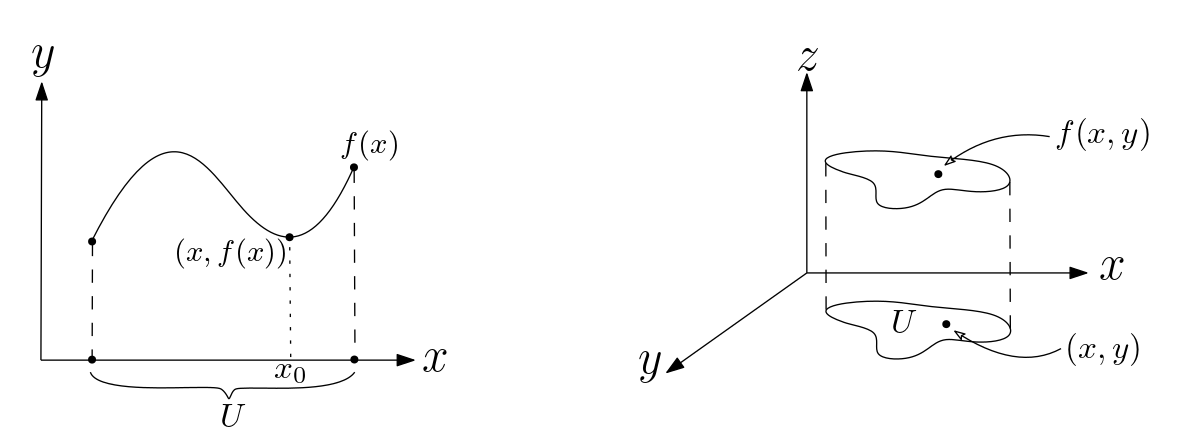
\includegraphics[width=\linewidth]{MATH314_Notes_Fig1.png}
		   		 	\captionsetup{margin=1cm, justification=raggedright}\caption{\textbf{a)} Two dimensional  interpretation, $f:U\subset \R \to \R$. \textbf{b)} Three dimensional interpretation, can be generalized to $f:U\subset \Rn \to \R$.}
		   		 \end{figure}  
	
	\begin{definition}
		Let $f: U \subset \Rn \to \R$ and let $ c\in \R $ .Then the level set of value $ c $ is defined to be the point $\vec{x} \in U$ which $f(\vec{x}) = c$. 
		\begin{align*}
			&\text{If } \ n =2 , \quad \text{we say level curves} \\
			&\text{If } \ n =3 , \quad \text{we say level surfaces}
		\end{align*}
	\end{definition}
	
	\begin{example}
		Describe the level curves of $f(x,y) = x^{2} + y^{2}$ .\\
		Recall that level curves live in $\mathbb{R}^{2}$ (in domain) \\
		Let $c = 1$ , $\xrightarrow \ x^{2} + y^{2} = 1^{2}$
		The level curves are circles of radius $\sqrt{c}$. 
	\end{example}
	
	\begin{example}
		Describe the level surfaces of $f(x,y,z) = x^{2} + y^{2} + z^{2}$ \\
		Let $c = 1$ , $\xrightarrow{} \ x^{2} + y^{2}+ z^{2} = 1$ (...). The level curves are spheres of radius $\sqrt{c}$. Note these are surfaces living in $\mathbb{R}^{3}$ space as illustrated in Figure 2a. 
	\end{example}
	\begin{figure}[H]
		   		 	\centering
		   		 	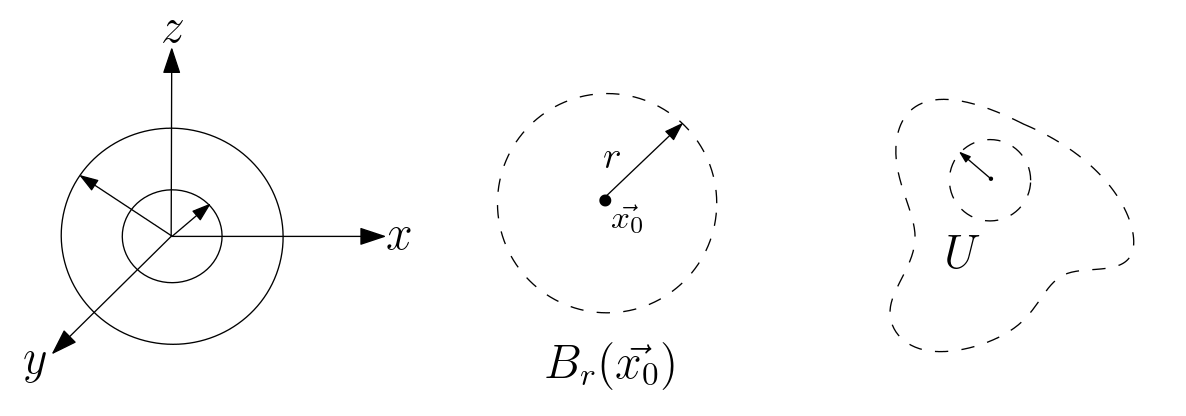
\includegraphics[width=0.9\linewidth]{MATH314_Notes_Fig2.png}
		   		 	\captionsetup{margin=1cm, justification=raggedright}\caption{\textbf{a)} Level curves in $\R^{3}$. \textbf{b)} Open ball of radius $r$ centered at $\vec{x_{0}}$.   \textbf{c)} Illustration of an open-set. }
		   		 \end{figure}
	
	\newpage \section{Limits and Continuity}
		Let $\vec{x_{0}} \in \Rn$ and let $ r $ be a positive real number. The open ball of radius $r$ centered at $\vec{x_{0}} $, as illustrated in Figure 2b, is defined as the set of all vectors $\vec{x}$ such that 
		$$\{\norm{\vec{x} - \vec{x_{0}}}  < r\}_{\text{distance between $\vec{x}$ and $\vec{x_{0}}$}}$$
		\begin{equation} 
		\underbrace{B_{r}(\vec{x_{0}})}_{\text{Ball centered at $r$}} = \{ \vec{x} \in \Rn \mid \norm{\vec{x} - \vec{x_{0}}} < r\} \label{Ball-centered}
		\end{equation}
		If $\norm{\vec{x} - \vec{x_{0}}} = r$ the $\vec{y} \notin B_{r}(\vec{x_{0}})$ i.e, the dotted line is not in the set.
		
	\begin{definition}[Open set]
		Let $U \in \Rn$ we call $ U $ an open set if for every point $\vec{x_{0}} \in U$ , there exists a $ r> 0$ such that $B_{r}(\vec{x_{0}}) \subset U$. \label{open-set}
	\end{definition}
	\noindent An attempt for a visual interpretation of Definition \eqref{open-set} is provided in Figure 2c.
	
	\begin{example}
		Prove that $(0,1) \cross (0,1)$ is an open set, where $$(0,1) \cross (0,1) = \{(x,y) \in \mathbb{R}^{2} \mid x\in (0,1) , y\in (0,1)\} $$.
		Take a point $(x_{0} , y_{0}) \in S \implies x_{0} \in (0,1) $ and $y_{0} \in (0,1)$
		\\
		\begin{align*}
			\text{Let  } r_{1} &= \min(x_{0} , 1 - x_{0}) \\
	 r_{2} &= \min(y_{0} , 1-y_{0}) \\
	 r &= \frac{\min(r_{1},r_{2})}{2} 
		\end{align*}
		By this construction, 
		\begin{equation*}
			\begin{split}
				(x_{0} -r , x_{0}+r) &\in (0,1) \\
				(y_{0} -r , y_{0}+r) &\in (0,1) 
			\end{split}
			\xrightarrow{} 
			\begin{split}
				\underbrace{(x_{0} -r , x_{0}+r) \cross (y_{0} -r , y_{0}+r)}_{\text{is an open square of radius $r$}}
			\end{split}
		\end{equation*}
		Moreover recalling \eqref{Ball-centered}, we can construct 
		$$ \underbrace{B_{r}(x_{0},y_{0}) }_{\mathclap{\text{open circle of radius $r$}}} \subset (x_{0} -r , x_{0}+r) \cross (y_{0} -r , y_{0}+r)$$
		Conclusion : $S$ as defined is open. \\
		"Idea is to show that there is a circle in there"
	\end{example}
	
	\begin{definition}[Neighborhood]
		We say a neighborhood of $\vec{x} \in \Rn$ is any  open set containing $\vec{x}$. \label{Neighbourhood}
	\end{definition}
	
	\begin{definition}[Boundary point]
		Let $A \subset \Rn$. A point $\vec{x} \in \Rn$ is called a boundary point of $A$ if every neighborhood of $\vec{x}$ contains points in $A$ and not in $A$. \label{Boundary point}
	\end{definition}
	
	\rule{\linewidth}{0.4 pt}
	
	\begin{definition}
		Let $ f: A \subset \Rn \to \Rm$ , where $A$ is open. Let $\vec{x_{0}} \in A$ or a boundary point of $A$ , and let $N$ be a neighborhood of $\vec{b} \in \Rm$ , we say $f$ is eventually in $N$ as $\vec{x} \to \vec{x_{0}}$ if there exists a neighborhood $U$ of $\vec{x_{0}}$ such that  \\
		if $\vec{x} \neq \vec{x_{0}} $ , $\vec{x} \in U$ and $\vec{x} \in A$ (in the domain) 
		$\implies f(\vec{x}) = N$ .
		We say $f\to \vec{b}$ as $\vec{x} \to \vec{x_{0}}$ 
		\begin{equation} 
		\text{i.e,} \quad \lim_{\vec{x} \to \vec{x_{0}}} f(\vec{x}) = \vec{b}  \label{limit-to-constant}
		\end{equation}
		this happens when given any neighborhood of $N$ of  $\vec{b}$ $f$ is eventually in $N$ as $\vec{x} \to \vec{x_{0}}$ (approaches $\vec{x_{0}}$) \\
		$\implies$ it may be that $\vec{x} \to \vec{x_{0}}$ that the values of $f(\vec{x})$ do not get close to any particular number.In this case the limit DNE. 
	\end{definition}
	
	\begin{figure}[h]
		\begin{minipage}[!]{0.45\linewidth}
			\begin{align*}
				\vspace{-1cm}
				&\text{Let $A = (\alpha, \beta)$ an open interval.} \\
				&\text{-Pick a random point $x_{0} ,b$} \\
				&\text{-Now pick any neighbourhood of $b$} \\
				&\text{-If i put any $x$ in the set $U$ then $f(x) \in N$.} \\
				&\text{-$U \subset A$} 
			\end{align*}
		\end{minipage}
		\hfill 
		\begin{minipage}[!]{0.45\linewidth}
				\centering{
						\includegraphics[width=\linewidth]{calc_3_1d_interpretation.png}
						\captionsetup{margin=1cm, justification=raggedright}\caption{1-D interpretation}
						}
		\end{minipage}
	\end{figure}
	\begin{example}
		Use the idea of Definition \eqref{limit-to-constant} to show $$\lim_{x\to 0} f(x) \quad \text{DNE} $$
		where 
		\begin{equation*}
				f = 
			\begin{cases}
				1 \ \ & ,x > 0 \\
				0 \ \ & ,x = 0 \\
				-1 \ \ & ,x < 0
			\end{cases}
			\qquad \to
			\begin{align}
				&\text{Limit from the right $\neq $ limit from the } \\ &\text{left so DNE ,from calc.1} 
			\end{align}
		\end{equation*}
		Take any open-set $U$ containing $0$, for example : $U = (-r, r) , r> 0$ .Then for any $r$ , if $ {x<0 }$ and ${ x \in U  \implies f(x) = -1}$.
		If ${ x>0 }$ and ${x \in U  \implies f(x) = 1}$. Therefore , the elements of $U$ aren't approaching a particular value for any $U$ containing $0$, thus DNE. Indeed, if it's elements are not approaching any \underline{single} value then DNE. 
		\end{example}
		
		\begin{definition}[Continuous]
		\label{continuous}
			Let $f : A \in \Rn \to \Rm $ and let $\vec{x_{0}} \in A $. We say $f$ is continuous at $\vec{x_{0}} $ if and only if 
			\begin{equation} 
			\lim_{\vec{x} \to \vec{x_{0}}} f(\vec{x}) = f(\vec{x_{0}})
			\end{equation}
			Saying $f$ is continuous means continuous at all points in its domain (not just $\vec{x_{0}}$). 
		\end{definition}
		
		\begin{theorem}
		
			Let $f : A \subset \Rn \to \Rm , \ g: A \subset \Rn \to \Rm $ and $ c\in \R$ .
			\begin{enumerate}[label=(\roman*)]
				\item If $f$ is continuous at $\vec{x_{0}}$, then so is the function $cf = cf(x)$ (i.e scalar multiplication doesn't affect continuity).\label{(i)}
				\item If $f,g$ are continuous at $\vec{x_{0}}$, then so is $(f+g)(\vec{x}) = f(\vec{x}) + g(\vec{x})$ is continuous at $ \vec{x_{0}} $ \label{(ii)}
				\item If $f(\vec{x} = (f_{1}(\vec{x}) + f_{2}(\vec{x}) , \dots , f_{m}(\vec{x})))$ then $f$ is continuous at $\vec{x_{0}}$ if and only if each real-valued function $f_{1}(\vec{x}) \quad i= 1,\dots, m$ is continuous at $\vec{x_{0}}$ \label{(iii)}
				\item If $m=1 $ and $f, g $ real valued and \label{(iv)}
				\begin{gather*}
					\lim_{\vec{x}\to \vec{x_{0}}} f(\vec{x}) = a , \ \ \lim_{\vec{x}\to \vec{x_{0}}}g(\vec{x}) =b \ 
					\implies  \lim_{\vec{x}\to \vec{x_{0}}} f(\vec{x})g(\vec{x}) = ab
				\end{gather*}
			\end{enumerate}
		\end{theorem}
		
		\begin{example}
			Show that $f(x,y) = \left(x^{2}y, \dfrac{y+x^{3}}{1+x^{2}}\right)$ is continuous using Theorem 2.1. \\
			Let $f_{1}(x,y) = x^{2}y$ and let $f_{2}(x,y) =  \dfrac{y+x^{3}}{1+x^{2}}$ , then by \ref{(iii)} ,we need to show that $f_{1} $ and  $f_{2} $ are continuous. 
			\begin{align*}
				& f_{1} (x,y) = x^{2}y \qquad , x^{2} \ \text{and} \ y \ \text{are both polynomials} \implies \text{continuous.} 
				\intertext{Also, by \ref{(iv)}, the product is also continuous}
				& f_{2} (x,y) = \dfrac{y+x^{3}}{1+x^{2}} = \underbrace{(y+x^{3})}_{\mathclap{\text{sum of cont. functions $\checkmark$}}}\left(\frac{1}{1+x^{2}}\right).
  			\end{align*}
  			For $1/(1+x^{2})$ the denominator is never $0$ so by Theorem 2.1, is continuous.\\
  			Conclusion: by  \ref{(iv)} ,$\ \ f_{2}(x,y) $ is continuous $\implies f $ is continuous as well by \ref{(iii)}.
		\end{example}
		\begin{theorem}
			Let $g : A \subset \Rn \to \Rm , \ f: B\subset \Rm \to \mathbb{R}^{p}$. \\
			Suppose $g(A) \subset B$  (i.e $B$ much larger than the range of $g$ so that $f \circ g$ is defined on $A$.) \\
			If $g$ is continuous at $\vec{x_{0}} \in A$ and f is continuous at $ \vec{y_{0}} = g(\vec{x_{0}}) $, then $f\circ g$ is continuous at $ \vec{x_{0}} $.
		\end{theorem}
		
		\begin{figure}[H]
				\centering
				\includegraphics[width=0.9\linewidth]{calc_3_fg_diagram.png}
				\captionsetup{margin=1cm, justification=raggedright}\caption{Visual picture for comprehension.}
		\end{figure}
		
		\begin{example}
			Show that  $f(x,y,z) = (xy + z)^{2} + (\cos(y))^{3}$ is continuous. \\
			We first and foremost define $f_{1} = (xy + z)^{2}$ and $f_{2} =  (\cos(y))^{3}$.\\
			Say $f_{1}(x,y,z) = F_{1}(G_{1}(x,y,z)), \quad G_{1} : \mathbb{R}^{3} \to \R  , \ F_{1}: \R \to \mathbb{R}^{3}$. \\
			So $G_{1} (x,y,z) = xy + z $ is continuous (polynomial and product) by \ref{(ii)} and \ref{(iv)}. \\
			$ f_{1}(x) =x^{2}$ is continuous because it is also a polynomial , therefore $f_{1} $ is continuous by Theorem 2.1. \\
			\\
			Similarly, we define $f_{2}(x,y,z) = F_{2}(G_{2}(x,y,z)) ,  \  G_{2} : \mathbb{R}^{3} \to \R , \ \ F_{2} : \R \to \R$ . \\
			Where $G_{2}(x,y,z) = \cos(y) $ , which is obviously continuous. $F_{2}(x) = x^{3}$ is also continuous so by same analysis $f$ is continuous as well.  
		\end{example}
		
		\subsection{Limit Review}
		
		\begin{example}
			Compute $$ \lim_{(x,y) \to (0,0)} \frac{x^{4} \arctan(\dfrac{1}{x^{2}+y^{2}})}{x^{2}+y^{2}}.$$
			Let us show that it exists (intuitively) using polar coordinates. 
			\begin{equation*}
				\begin{split}
					x &= r \cos \theta \\
					y &= r \sin \theta
				\end{split}
				 \ \ \implies \ \
				\begin{split}
					&= \lim_{r \to 0} \frac{r^{4}(\cos\theta)^{4} \arctan(\dfrac{1}{r^{2}})}{r^{2}} \\
					&= \lim_{r \to 0} r^{2}(\cos \theta )^{4} \underbrace{\arctan(\dfrac{1}{r^{2}})}_{= \pi/2} \\
					&= \frac{\pi}{2} \underbrace{\lim_{r \to 0} r^{2} (\cos\theta )^{4}}_{\text{Squeeze it !}}
				\end{split}
			\end{equation*}
			\begin{equation*}
				0 \le (\cos\theta)^{4} \le 1 \  \implies \ 0 \le \lim_{r\to 0} r^{2}(\cos\theta )^{4} \le \underbrace{\lim_{r \to 0} r^{2}}_{=0}
			\end{equation*}
			Finally we conclude that the limit ,as defined, converges to $0$.
		\end{example}
		
		\begin{example}
			Compute 
			$$ \lim_{(x,y) \to (0,0)} \frac{x^{6}y^{3}}{x^{12}+x^{6}}$$
			\textbf{Step 1 :} Show that limit exists when approaching $(0,0)$ along any line. Set $y= mx$.
			\begin{equation*}
				\lim_{x \to 0} \frac{x^{6}(mx)^{3}}{x^{12}+(mx)^{6}}= m^{3} \lim_{x\to 0} \frac{x^{9}}{x^{12}+x^{6}m^{6}} = m^{3} \lim_{x\to 0} \frac{x^{3}}{x^{6} + m^{6}}
			\end{equation*}
			The numerator goes to $0$ and the denominator goes to $0+m^{6}$, but if $y=0$ then $\lim = 0$.\\
			Therefore, the limit equals zero when approaching any line since we arbitrarily chose $mx \quad , m \in \R$. \\
			\textbf{Step 2 : } Let $y = x^{2}$ 
			\begin{equation*}
				\lim_{x\to 0} \frac{x^{6}(x^{2})^{3}}{x^{12}+(x^{2})^{6}} = \frac{x^{12}}{x^{12}+x^{12}} = \frac12 
			\end{equation*} 
			Different result $1/2 \neq 0 \implies $ limit DNE. 
		\end{example}
		
		\newpage \section{Differentiation}
			Let $f: U \subset \Rn \to \R$ (real-valued) \\
			\begin{equation*}
				\begin{split}
					\text{Then } \ \pdv{f}{x_{1}} , \dots , \pdv{f}{x_{n}} 
				\end{split}
				\quad 
				\begin{cases}
					\parbox{8cm}{the partials of $f$ with respect to its first, second and $n$'th variables , are all real-valued functions of $n$ variables.}
				\end{cases}
			\end{equation*}
			i.e, $\pdv{f}{x_{i}} : \Rn \to \R \quad i = 1 , \dots ,n $ which at point $\vec{x} = (\vec{x_{1}} , \dots, \vec{x_{n}})$ are defined by 
			$$ \pdv{f}{x_{j}} (x_{1}, \dots, x_{n}) = \lim_{h \to 0} \frac{f(x_{1},x_{2},\dots, x_{j+h},\dots ,x_{n}) - f(x_{1},\dots , x_{n})}{h}.$$
			Note that this may be written shorter, 
			$$ \lim_{h\to 0  } \frac{f(\vec{x} + \vec{e}_{j}h) - f(\vec{x})}{h} \quad \text{where, } \vec{e}_{j} = (0,0, \dots ,\underbrace{1}_{\mathclap{\text{$j^{\text{th}}$ component}}} ,\dots , 0).$$
 			Extra information : $\vec{e}_{j}  $ may be seen a standard basis vector.
 			
 			\begin{example}
 				$$ f(x_{1},x_{2},x_{3},x_{4},x_{5}) = x_{1}^{2}x_{3} + x_{4}\sin(x_{1}x_{2})$$
 				is continuous.
 				$$ \pdv{f}{x_{1}} = 2x_{1}x_{3} + x_{4}\cos(x_{1}x_{2})x_{2}$$
 				is also continuous and works for the other $x_{i}$ as well.
 			\end{example}
 			
 			\begin{example}
 				Let $f(x,y) = x^{\sfrac{1}{3}}x^{\sfrac{1}{3}}$ . Compute $f_{x}(0,0)$.
 				$$ f_{x}(0,0) = \lim_{h\to 0} \frac{f(h,0)- f(0,0) }{h} = \lim_{h\to 0} \frac{0}{h} = 0 \quad \text{the right answer} \checkmark$$
 				Note that if we would had computed $f_{x}(x,y) =  \frac{1}{3}x^{\sfrac{-2}{3}} y^{\sfrac{1}{3}}$, at $(0,0)$ it cannot be evaluated. \\
 				$\to$ So we conclude that simply having partials exist at a point is not enough to have differentiability.
 			\end{example}
 			
 	\rule{\linewidth}{0.4 pt}
 	
 	\noindent We ended last time by studying the function 
 	\begin{equation*}
 		\begin{rcases}
 			f(x,y) &= x^{1/3}y^{1/3} \\
 			f_{x}(0,0) &= 0 , \ \  f_{y}(0,0) = 0 
 		\end{rcases}
 		\qquad \text{,but we don't expect $f(x,y)$ to be differentiable at $(0,0)$.}
 	\end{equation*}
 	In Calculus 1, we say $f$ is differentiable at $x_{0}$ if 
 	$$ \lim_{h\to 0  } \frac{f(x_{0}+h)-f(x_{0})}{h}\qquad \text{exists}.$$
 	Therefore we said that that 
 	\begin{equation} 
 	 f^{\prime}(x_{0}) =  \frac{f(x_{0}+h)-f(x_{0})}{h}\quad , \text{for some} \ f^{\prime}(x_{0}) \in \R, \label{f_differentiable}
 	 \end{equation}
 	so $f$ is differentiable at $x_{0}$ if such a number $f^{\prime}(x_{0})$ exists to satisfy the limit.
 	\begin{figure}[H]
 		   		 	\centering
 		   		 	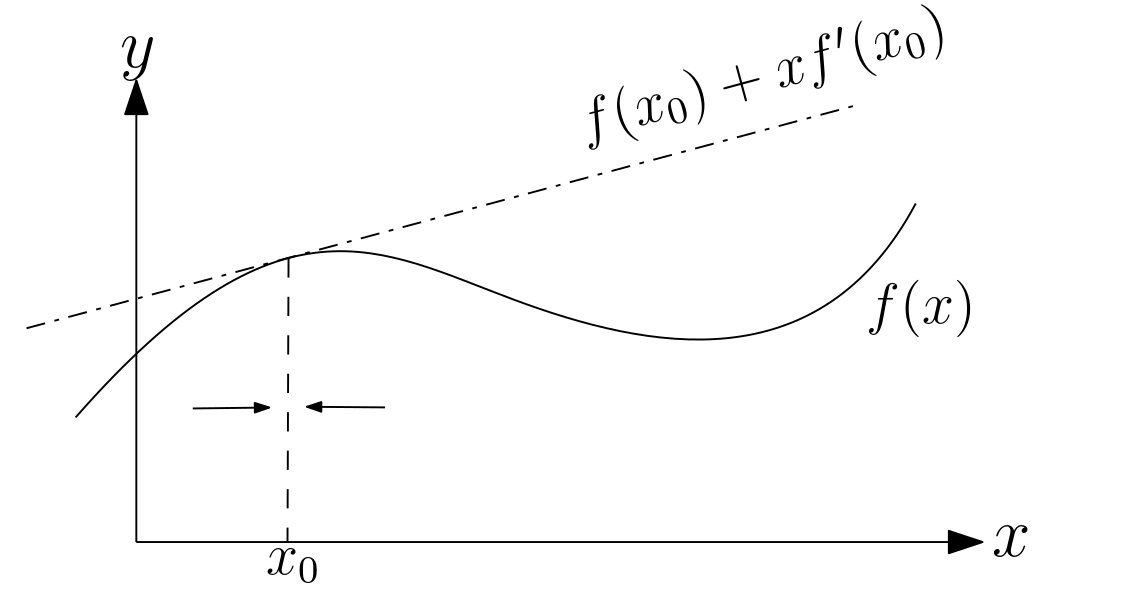
\includegraphics[width=0.6\linewidth]{MATH314_Notes_Fig3.png}
 		   		 	\captionsetup{margin=1cm, justification=raggedright}\caption{Tangent line to a function following (3.0.1).}
 		   		 \end{figure}
 	
 	\begin{example}
 		Using the definition of differentiability of real-valued function, show that for $f(x) = x^{3}$ that $f^{\prime}(x) = 3x^{2}$.
 		\begin{align*}
 			&\lim_{h \to 0} \frac{(x_{0}+h)^{3} -x_{0}^{2}-(3x_{0}^{2})h}{h}\\
 			&= \lim_{h \to 0} \frac{(x^{3}+3x_{0}h + 3x_{0}h +h^{3}) - x_{0}^{3} -(3x_{0}^{2})h}{h}\\
 			&= \lim_{h \to 0}\frac{x_{0}h^{2}+h^{3}}{h} \\
 			&= \lim_{h \to 0} 3x_{0}h+h^{2} =0
 		\end{align*}
 		Conclusion : $f$ as defined , is indeed differentiable.
 	\end{example}
 	
 	\noindent Now what about $f: \R^{2} \to \R$ functions?
 	\begin{definition}
 		We say $f:\R^{2} \to \R $ is differentiable at $(x_{0},y_{0})$ if $f_{x}(x_{0},y_{0})$ and $f_{y}(x_{o},y_{0})$ exist and 
 		\begin{equation}
 			\lim\limits_{(x,y) \to (x_{0},y_{0})} f(x,y) =\frac{ f_{x}(x_{0},y_{0})-(f_{x})(x_{0},y_{0})(x-x_{0}) +f_{y}(x_{0},y_{0})(y-y_{0})}{\norm{(x,y) - (x_{0},y_{0})}}. \label{differentiability_R2}
 		\end{equation}
 	\end{definition}
 	\noindent Recall that the tangent plane to a function $z=f(x,y) $ at some point $P(x_{0},y_{0},z_{0})$ is 
 	 		\begin{equation} 
 	 		 (z-z_{0}) = f_{x}(x_{0},y_{0})(x-x_{0}) + f_{y}(x_{0},y_{0})(y-y_{0}). \label{tangent-plane}
 	 		 \end{equation}
 	
 	\begin{note}
 		The definition of a tangent plane \eqref{tangent-plane} requires $f_{x}(x,y)$ and $f_{y}(x,y)$ to be continuous at $(x_{0},y_{0})$, however our definition of differentiability doesn't require this.
 	\end{note}
 	
 	\begin{example}
 		Using the definitions of partial derivatives and differentiability , show that $f(x,y) = x^{2}+y^{4}+xy$ is differentiable at $(x,y) = (1,0)$. 
 		
 		\noindent If we compute $f_{x}$ and so on, we assume continuity but, 
 		\begin{alignat*}{2} 
 			f_{x}(1,0) &= \lim_{h \to 0} \frac{f(1+h, 0)-f(1,0)}{h} &= \lim_{h\to 0} \frac{(1+h)^{2}-1}{h} \\
 			&= \lim_{h \to 0} \frac{1+2h}+h^{2}-1{h} &= \lim_{h\to 0} 2+h = 2 \\
 			f_{y}(1,0) &= \lim_{h\to 0} \frac{f(1,h) -f(1,0)}{h} &= \lim_{h \to 0}\frac{1+h^{4}+h-1}{h} \\
 			& =\lim_{h \to 0} \frac{h^{4}+h}{h} = 1
 		\end{alignat*}
 		Now we compute the final limit : 
 		\begin{align*}
 			&= \lim_{(x,y) \to (1,0)} \frac{f(x,y)-f(1,0)-(f_{x}(1,0)(x-1)+f_{y}(1,0)y)}{\norm{(x,y)}-(1,0)} \\
 			&= \lim_{(x,y) \to (1,0)} \frac{(x^{2}+y^{4}+xy) -(1)-(2(x-1)+y)}{\underbrace{\sqrt{(x-1)^{2}+y^{2}}}_{\text{Euclidian Norm !}}}\\
 			&= \lim_{(x,y) \to (1,0)} \frac{x^{2}+2x +1 +y^{4}-y+xy}{\sqrt{(x-1)^{2}+y^{2}}}\\
 			&= \lim_{(x,y) \to (1,0)} \frac{(x-1)^{2}+y^{4} -y +xy}{\underbrace{\sqrt{(x-1)^{2}+y^{2}}}_{\text{Relabel } \ x\to x-1}} \\
 			\intertext{Thus, the limit now goes to $(0,0)$ ; } 
 			&= \lim_{(x,y) \to (0,0)} \frac{x^{2}+y^{4}-y+(x+1)y}{\sqrt{x^{2}+y^{2}}} = \lim_{(x,y) \to (0,0)} \frac{x^{2}+y^{4}+xy}{\sqrt{x^{2}+y^{2}}}\\
 			\intertext{Now we transform to polar coordinates - Set $x= r\cos \theta $ and $y = r\sin \theta$,} 
 			&= \lim_{r\to 0} \frac{r^{2}\cos^{2}\theta + r^{4}\sin^{4}\theta + r^{2}\cos \theta \sin \theta}{r} \\
 			&= \lim_{r\to 0} r\cos^{2}\theta +r^{3}\sin^{4}\theta +r\cos\theta\sin\theta = \boxed{0}
 	 	\end{align*}
 	 	Conclusion : $f$ as defined, is differentiable at $(1,0)$. Note that regardless of the value for $\theta$ , $r$ dominates and goes to zero. Therefore, just like $mx$ in Example 2.6 where we wanted the limit to come from "all sides", here all directions ($\theta$) point to zero.
 	\end{example}
 	
 	\begin{example}
 		Show that $f(x,y) = x^{1/3}y^{1/3}$ is differentiable at $(0,0)$ (question from last class). 
 		
 		\noindent \textbf{Recall :} We found that $f_{x}(0,0) = 0 = f_{y}(0,0)$.
 		\begin{align*}
 			&= \lim_{(x,y) \to (0,0)} \frac{f(x,y) -f(0,0) - (f_{x}(0,0)x + f_{y}(0,0)y)}{\norm{(x,y)} - (0,0)} \\
 			&= \lim_{(x,y) \to (0,0)} \frac{x^{1/3}y^{1/3} -0 -0 -0}{\sqrt{x^{2}+y^{2}}} \\
 			&= \lim_{(x,y) \to (0,0)} \frac{x^{1/3}y^{1/3}}{\sqrt{x^{2}+y^{2}}}
 		\end{align*}
 		Note that because the numerator power is $2/3$ we expect the expression to blow up to $\infty$.\\
 		Moreover, note that this example works with both polar and $y=mx$ methods.\\
 		Let us try setting $y=mx$. 
 		\begin{alignat*}{2}
 			\implies &= \lim_{x \to 0} \frac{x^{1/3}(mx)^{1/3}}{\sqrt{x^{2}+(mx)^{2}}} = \lim_{x\to 0} \frac{m^{1/3}x^{2/3}}{\abs{x}\sqrt{1+m^{2}}} \\
 			&= \lim_{x\to 0} \underbrace{\frac{1}{\abs{x}^{1/3}}}_{\text{goes to } \infty} \frac{m^{1/3}}{\underbrace{\sqrt{1+m^{2}}}_{\mathrlap{
 			\begin{align}
 				\text{if} \  &m \ \textless \ 0 \implies - \infty \\
 				&m \ \textgreater \ 0 \implies +\infty 
 			\end{align}}}} \ \ \implies \text{goes to } \ \pm \infty 
 		\end{alignat*}
 		Conclusion : $f$ as defined, is differentiable at $(0,0)$.
  	\end{example}
  	
  	\begin{note}
  		We can rewrite the differentiability limit as 
  		\begin{equation} 
  		\lim_{(x,y) \to (x_{0},y_{0})} \frac{f(x,y) -f(x_{0},y_{0}) - \overbrace{[f_{x}(x_{0},y_{0}) f_{y}(x_{0},y_{0})]}^{\text{define } = D{f}(x_{0},y_{0})} \begin{bmatrix}
  			x-x_{0} \\
  			y-y_{0}
  		\end{bmatrix}}{\norm{(x,y)-(x_{0},y_{0})}}. \label{differentiability_D}
  		\end{equation}
  		$D{f}$ here is called the derivative of $f$ , but also here 
  		$D{f} = \nabla f \quad $ (gradient). More generally, we can write
  		\begin{equation} 
  		\text{for , }  f: \Rn \to \R \quad, \lim_{\vec{x} \to \vec{x_{0}}} \frac{f(\vec{x}) - f(\vec{x_{0}}) - \nabla f(\vec{x}-\vec{x_{0}})}{\norm{\vec{x}-\vec{x_{0}}}}. \label{differentiability_generalized}
  		\end{equation}
  	\end{note}
  	
  	\begin{definition}
  		Let $U$ be an open set of $\Rm$ and let $f : U \subset \Rn \to \Rm$ we say $f$ is differentiable at $\vec{x_{0}} \in U$ if the partials of $f$ exist and if  \label{differentiability_in_open_set}
  		\begin{equation} 
  		\lim_{\vec{x} \to \vec{x_{0}}} \frac{\norm{f(\vec{x}) - f(\vec{x_{0}}) - T(\vec{x}- \vec{x_{0}})}}{\norm{\vec{x}-\vec{x_{0}}}} = 0, \label{eq_differentiability_in_open_set}
  		\end{equation} 
  		for some matrix $T$ (Linear transformation).
  	\end{definition}
  	
  	\begin{theorem}
  	\label{thm_Df}
  		$T=D{f}(\vec{x_{0}})$ is the partial derivatives matrix of \\ ${f(\vec{x_{0}}) = (f_{1}(\vec{x_{0}}), f_{2}(\vec{x_{0}}), \dots , f_{m}(\vec{x_{0}}))},$
  		\begin{equation} T = D{f}(\vec{x_{0}}) = 
  		\begin{bmatrix}
  			\pdv{f_{1}}{x_{1}} \dots \pdv{f_{1}}{x_{n}} \\
  			\vdots \quad \vdots \\
  			\pdv{f_{m}}{x_{1}} \dots \pdv{f_{m}}{x_{n}}
  		\end{bmatrix}. \label{eq_Df}
  		\end{equation}
  	\end{theorem}
  	
  	\begin{proof}
  		Suppose this limit is true  i.e., it is equal to $0$. \\
  		Recall from linear algebra that $(\norm{\vec{x}} = 0 \implies \vec{x} = 0)$ which implies each component goes to $0$ as well.
  		Let us rewrite \eqref{eq_differentiability_in_open_set}: 
  		\begin{align*}
  			&\lim_{\vec{x} \to \vec{x_{0}}} \frac{\abs{f_{i}(\vec{x}_{0}) -f_{i}(\vec{x_{0}}) - (T(\vec{x} -\vec{x_{0}})_{i})}}{\norm{\vec{x} - \vec{x_{0}}}} = 0 \quad, \forall i = 1,\dots ,m \\
  			\intertext{Set $\vec{x_{0}} +\vec{h} = \vec{x}$,}
  			&\lim_{\vec{h}\to \vec{0}}\frac{\abs{f_{i}(\vec{x_{0}}+\vec{h}) -f_{i}(\vec{x_{0}}) -(T(\vec{h}))_{i}}}{\norm{\vec{h}}} = 0 \\
  			\intertext{This limit holds along any path $\vec{h} \to \vec{0}$. Now  set $\vec{h} = (0,0,\dots,a, \dots,0) = \underbrace{a\vec{e}_{j}}_{\mathclap{\text{standard basis vector}}}$,} 
  			&\lim_{a \to 0} \frac{\abs{f_{i}(\vec{x_{0}} + a\vec{e}_{j}) - f_{i}(\vec{x_{0}}) - (Ta\vec{e}_{j})}}{\abs{a}} = \lim_{a\to 0} \frac{\abs{f_{i}(\vec{x_{0}} + a\vec{e}_{j}) -f_{i}(\vec{x_{0}}) - a(T\vec{e}_{j})_{i}}}{\abs{a}} \\
  			&= \lim_{a\to 0} \abs{\frac{f_{i}(\vec{x_{0}} + a\vec{e}_{j}) - f_{i}(\vec{x_{0}}) - a(T\vec{e}_{j})_{i}}{a}} = \lim_{a\to 0} \abs{\frac{f_{i}(\vec{x_{0}} + a\vec{e}_{j}) - f_{i}(\vec{x_{0}})}{a} -(T\vec{e}_{j})_{i}} \\
  			&= \lim_{a\to 0} \frac{f_{i}(\vec{x_{}} + a\vec{e}_{j}) -f_{i}(\vec{x_{0}})}{a} = (T\vec{e}_{j})_{i} \\
  			& \quad \implies \pdv{f_{i}}{x_{j}} = (T\vec{e}_{})_{i} = (i,j)^{\text{th}} \ \text{component of } \ T.
  		\end{align*}
  		Conclusion : $T$ is the matrix of partials also known as the \underline{Jacobian} of $f$.
    \end{proof}
    
  	\rule{\linewidth}{0.4 pt}
  	\\
  	Last time we introduced the notation of differentiability for functions $f: U \subset \Rn \to \Rm$ , where $f$ is differentiable at $\vec{x_{0}} \in \Rn$ provided that all partials exist and recalling \eqref{eq_differentiability_in_open_set}
  	$$ \lim_{\vec{x} \to \vec{x_{0}}} \frac{\norm{f(\vec{x}) - f(\vec{x_{0}}) - D{f}(\vec{x}-\vec{x_{0}})}}{\norm{\vec{x} - \vec{x_{0}}}}= 0.$$ \\
  	Where $D{f}$ is the Jacobian matrix of $f$, with $(D{f})_{ij} = \dfrac{\partial f_{i}}{\partial x_{j}}$.
  	
  	\begin{theorem}[Continouity for real-valued functions]
  		Let $f : U \subset \Rn \to \Rm$ and let $f$ be differentiable at $\vec{x_{0}} \in \Rn$, then $f$ is continuous at $\vec{x_{0}}$.\label{thm-continouity}
  	\end{theorem}
  	
  	\begin{theorem}[Differentiability for real-valued functions]
  		Let $f : U \subset \Rn \to \Rm $. Suppose all partials $\sfrac{\partial f_{i}}{\partial x_{j}}$ exist and are continuous in a neighborhood of a point $\vec{x_{0}} \in U$. Then $f$ is differentiable at $\vec{x_{0}}$.\label{thm-differentiability}
  	\end{theorem}
  	
  	\begin{note}
  		\fbox{Continuous partials $\implies$ Differentiability $\implies$ Partials exist.} \\
  		
  		
  		This is useful because if conditions are met, we don't have to worry about using the long limit formula.
  	\end{note}
  	
  	\begin{figure}[H]
  		\centering
  		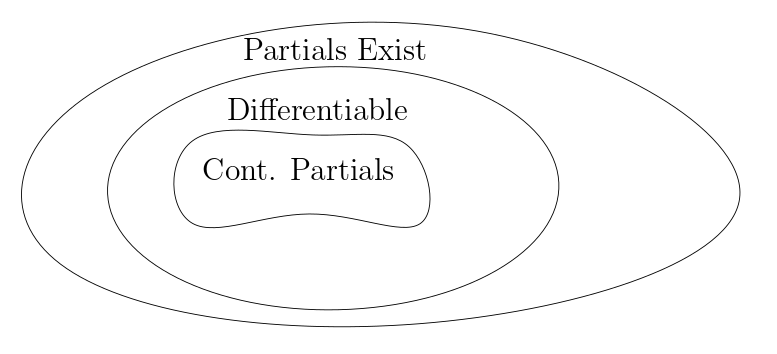
\includegraphics[width=0.7\linewidth]{MATH314_Notes_Hierarchical_Figure.png}
  		\captionsetup{margin=1cm}
  		\caption{Hierarchical inclusion of differentiability ,continuity and the partials associated. Note that within the differentiable set, functions have varying tangent plane.}
  	\end{figure}
  	
  	\begin{example}
  		Using the Theorems \ref{thm-continouity} and \ref{thm-differentiability}, show that $f(x,y) = \dfrac{xy}{(x^{2}+y^{2})^{2}}$ is differentiable at all $(x,y) \neq (0,0)$. 
  		\begin{equation*}
  			f_{x} = \frac{y(x^{2}+y^{2})^{2} -xy(2(x^{2}+y^{2})2x)}{(x^{2}+y^{2})^{4}} ,\ \ f_{y} = \frac{x(x^{2}+y^{2})^{2} -xy(2(x^{2}+y^{2})2y)}{(x^{2}+y^{2})^{4}}.
  		\end{equation*}
  		Both the numerator and denominator are continuous $\implies$ $f_{x}$ and $f_{y}$ are continuous  whenever $(x^{2}+y^{2})\neq 0$. Therefore, they're continuous away from $(0,0)$. Thus, we conclude that, since $f_{x}$ and $f_{y}$ are continuous $\forall (x,y) \neq (0,0) \implies f$ is differentiable at all $(x,y) \neq (0,0)$.
  	\end{example}
  	
  	\begin{example}
  		Using the derivative , find a function $f(x,y)$ and approximate \\ ${(0.99)^{3} + (2.01)^{3} - 6(0.99)(2.01)}$. \\
  		
  		\noindent Let $f(x,y) = x^{3} + y^{3}-6xy$ , which is obviously differentiable $\forall (x,y) \in \R^{2}$.\\ 
  		Points in a neighborhood of $(x,y)$ are well approximated by the tangent plane of $f$. Let $x=1$ ,$y=2$, $\Delta x = 0.01$ and $\Delta y = 0.01$.Then ,
  		$$ f(x-\Delta x , y + \Delta y ) \approx f(x,y) + f_{x}(x,y)(-\Delta x) + f_{y}(x,y)(+\Delta y) $$
  		\begin{alignat*}{2}
  			f_{x}(x,y) &= 3x^{2}-6y \implies  f_{x}(1,2) = 3-12 = \boxed{-9} \\
  			f_{y}(x,y) &= 3y^{2} -6x \implies f_{y}(1,2) = 12-6 = \boxed{6} \\
  			& \quad \implies f(1,2) = 1+8 -12 = \boxed{-3}.
  		\end{alignat*}
  		Now put the $\Delta x, \Delta y$  results in the initial expression, get 
  		\begin{equation*}
  			\implies f(0.99, 2.01) \approxeq -3 + (-9)(-0.01) + (6)(0.01) \approxeq -2.85.
  		\end{equation*}
  	\end{example}
  	
  	\newpage \section{Properties of Derivatives} 
  		Suppose $z = f(u(x),v(x), w(x))$ , where $u,v,w : \R \to \R$. Then , 
  		\begin{equation} 
  		\pdv{z}{x} = \pdv{f}{u}\pdv{u}{x} +\pdv{f}{v}\pdv{v}{x} + \pdv{f}{w}\pdv{w}{x}. \label{chain_rule}
  		\end{equation}
  		This is the classic chain rule as discussed in Calculus 3. Here we will generalize the concepts of differentiation to functions $f : \Rn \to \Rm$. 
  		
  		\begin{enumerate}
  			\item \textbf{The Constant Multiple Rule} \\
  			Let $f: U \subset \Rn \to \Rm$ be differentiable at $\vec{x_{0}} \in \Rn$ and let $c\in \R$. Then letting $h(\vec{x}) = cf(\vec{x})$ , 
  			\begin{equation} 
  			D{h}(\vec{x_{0}}) = cD{f}(\vec{x_{0}}). \label{eq_cosntant_multiple_rule}
  			\end{equation}
  			\item \textbf{The Sum Rule} \\
  			Let $f: U \subset \Rn \to \Rm$ and $g: U\subset \Rn \to \Rm$ ,which are both differentiable at $\vec{x_{0}}$. Then, $h(\vec{x}) + g(\vec{x})$ is also differentiable with 
  			\begin{equation}
  			 D{h}(\vec{x_{0}}) = D{f}(\vec{x_{0}}) +D{g}(\vec{x_{0}}). \label{eq_sum_rule}
  			\end{equation}
  			\begin{proof}
  				\begin{align*}
  					&\lim_{\vec{x} \to \vec{x_{0}}} \frac{\norm{h(\vec{x}) -h(\vec{x_{0}}) - (D{f}(\vec{x_{0}}) + D{g}(\vec{x_{0}}) ) (\vec{x}-\vec{x_{0}})}}{\norm{\vec{x}-\vec{x_{0}}}} \\
  					\intertext{Using $h(\vec{x}) = f(\vec{x}) + g(\vec{x})$,}
  					&= \lim_{\vec{x}\to \vec{x_{0}}} \frac{\norm{f(\vec{x}) -f(\vec{x_{0}}) - D{f}(\vec{x_{0}})(\vec{x}-\vec{x_{0}}) +g(\vec{x_{0}}) -D{g}(\vec{x_{0}})(\vec{x}-\vec{x_{0}})}}{\norm{\vec{x}-\vec{x_{0}}}} \\
  					\intertext{Using the Triangel Inequality : $\norm{\vec{x}+\vec{y}} \le \norm{\vec{x}} + \norm{\vec{y}}$,}
  					&\le \lim_{\vec{x} \to \vec{x_{0}}} \bigg[\frac{\norm{f(\vec{x}) -f(\vec{x_{0}}) - D{f}(\vec{x_{0}})(\vec{x}-\vec{x_{0}}) }}{\norm{\vec{x}-\vec{x_{0}}}} + \frac{\norm{g(\vec{x}) -g(\vec{x_{0}}) - D{g}(\vec{x_{0}})(\vec{x}-\vec{x_{0}}) }}{\norm{\vec{x}-\vec{x_{0}}}}\bigg]\\
  					& \le 0 \implies D{h}(\vec{x_{0}}) = D{f}(\vec{x_{0}}) + D{g}(\vec{x_{0}}). 
  				\end{align*}
  			\end{proof}
  			\item \textbf{Product Rule} \\ Let $F : U \subset \Rn \to \R , \  g: U\subset \Rn \to R$ , both differentiable at $\vec{x_{0}}$. Let $h(\vec{x}) = f(\vec{x})g(\vec{x})$\\
  			$\implies h: U\subset \Rn \to \R$ and $h$ is differentiable 
  			\begin{equation} 
  			\underbrace{D{h}(\vec{x_{0}})}_{\text{vector}} = \underbrace{g(\vec{x_{0}})D{f}(\vec{x_{0}}) + f(\vec{x_{0}})D{g}(\vec{x_{0}})}_{\text{vector}}. \label{eq_product_rule}
  			\end{equation}
  			\item \textbf{Quotient Rule} \\
  			Let $f$ and $g$ as above. If $g \neq 0$  in a neighborhood of $\vec{x_{0}}$ , then $h$ is differentiable $(h(\vec{x}) = f(\vec{x})/g(\vec{x}))$ at $\vec{x_{0}}$ with 
  			\begin{equation} 
  			D{h}(\vec{x_{0}}) = \frac{g(\vec{x_{0}})D{f}(\vec{x_{0}}) - f(\vec{x_{0}}) D{g}(\vec{x_{0}})}{(g(\vec{x_{0}}))^{2}}. \label{eq_quotient_rule}
  			\end{equation}
  		\end{enumerate}
  		\begin{example}
  			\begin{equation*}
  				\begin{split}
  					\text{Let} \ \ \ \frac{h(\vec{x}) f(\vec{x})}{g(\vec{x})}
  				\end{split}
  					\text{, where} \ \  
  				\begin{cases}
  					f(\vec{x}) &= xy\cos(z) \\
  					g(\vec{x}) &= x^{2}+y^{2}
  				\end{cases}.
  			\end{equation*}
  			Compute $D{h}$.
  			\begin{align*}
  				h_{x}(x,y,z) &= \frac{y\cos(z)(x^{2}+y^{2}) - xy\cos(z)(2x)}{(x^{2}+y^{2})^{2}}\\
  				h_{y}(x,y,z) &= \frac{x\cos(z) (x^{2}+z^{2})}{(x^{2}+z^{2})^{2}} = \frac{x\cos(z)}{(x^{2}+y^{2})} \\
  				h_{z}(x,y,z) &= \frac{-xy\sin(z)(x^{2}+y^{2})-xy\cos(z)(2x)}{(x^{2}+y^{2})^{2}}
  			\end{align*}
  			\begin{equation*}
  				\begin{split}
  					D{h} = 
  					\begin{bmatrix}
	  					h_{x}(x,y,z)\\
	  					h_{y}(x,y,z)\\
	  					h_{z}(x,y,z)
  					\end{bmatrix}
  				\end{split}
  				\: \: \text{or} \ \
  				\begin{split}
  					D{f} &= (y\cos (z), x\cos (z) , -xy\sin(z)) \\
  					D{g} &= (2x, 0 ,2z) \\
  					D{h} &= \frac{(x^{2}+y^{2})(y\cos(z)),x\cos(z) -xy\sin(z)-xy\cos(z)(2x,0,2z)}{(x^{2}+y^{2})^{2}}.
  				\end{split}
  			\end{equation*}
  		\end{example}
  		
  		\subsection{Chain Rule}
  		Let $U\subset \Rn , V \subset \Rm$ be open. Let $g : U \subset \Rn \to \Rm$, $f: V \subset \Rm \to \R^{p}$ , be given such that $g$ maps $U \to V$ (to ensure $f\circ g $) is defined. Suppose $g$ is differentiable at $\vec{x_{0}}$, with 
  		$$ D(f\circ g)(\vec{x_{0}}) = \underbrace{D{f}(\vec{y_{0}})\cdot D{g}(\vec{x_{0}})}_{\text{Product of matrices}}.$$ 
  		\begin{align*}
  			\text{Take } \ h &= f\circ g \quad , g = (g_{1}(\vec{x}) , g_{2}(\vec{x}) , \dots. g_{n}(\vec{x})) \\
  			&= (f_{1}(g_{1},\dots,g_{m}) , f_{2}(g_{1},\dots, g_{m}) , \dots, f_{p}(g_{1},\dots ,g_{m}))
  		\end{align*}
  		\begin{equation*}
  			\implies \left(\pdv{h}{x_{1}}\right)_{1} = \left(\pdv{h}{x}\right)_{1,1} = \pdv{f_{1}}{g_{1}} \pdv{g_{1}}{x_{1}} + \pdv{f_{1}}{g_{2}} \pdv{g_{2}}{x_{1}} + \dots +\pdv{f_{1}}{g_{m}} \pdv{g_{m}}{x_{1}}
  		\end{equation*}
  		\begin{align*}
  			D{h} &= D{f}(\vec{y_{0}}) D{g}(\vec{x_{0}}) , \quad \text{where } \ \ \vec{g} = g(\vec{x_{0}}) \\
  			&= 
  			\begin{bmatrix}
  				\pdv{f_{1}}{g_{1}} & \pdv{f_{1}}{g_{2}} &\dots &\pdv{f_{1}}{g_{m}} \\
  				\vdots & & \ddots &\\
  				\pdv{f_{p}}{g_{1}}& &\dots& \pdv{f_{p}}{g_{m}}
  			\end{bmatrix}
  			\begin{bmatrix}
  				\pdv{g_{1}}{x_{1}}& \pdv{g_{2}}{x_{2}}& \dots &\pdv{g_{1}}{x_{n}} \\
  				\vdots & & \ddots &\\
  				\pdv{g_{m}}{x_{1}} & & \dots &\pdv{g_{m}}{x_{n}}
  			\end{bmatrix}\\
  			\implies (D{h})_{1,1} &= \pdv{f_{1}}{g_{1}} \pdv{g_{1}}{x_{1}} + \pdv{f_{1}}{g_{2}} \pdv{g_{2}}{x_{1}} + \dots + \pdv{f_{1}}{g_{m}} \pdv{g_{m}}{x_{1}} 
  			\intertext{These are the same. }
  		\end{align*}
  		\vspace{-2cm}
  		\begin{example}
  			Let $f(x,y) = (\cos(y) + x^{2} , e^{xy}) , g(u,v) = (e^{u^{2}} , v-\sin(a))$. Compute $D(f\circ g)(0,0)$.
  			\begin{align*}
  				D(f\circ g)(0,0) &= D{f}(g(0,0))\cdot D{g}(0,0) \\
  				D{g}(0,0) &= 
  				\begin{bmatrix}
  					2ue^{u^{2}} & 0 \\
  					\cos(u) & 1 
  				\end{bmatrix}\bigg|_{(u,v) = (0,0)}
  				\ \ = 
  				\begin{bmatrix}
  					0 & 0 \\
  					-1 & 1
  				\end{bmatrix} \\
  				D{f}(g(0,0)) &= 
  				\begin{bmatrix}
  					2x & -\sin(y) \\
  					y & xe^{xy} 
  				\end{bmatrix}\bigg|_{g(0,0) = (1,0)}
  				\ \ = 
  				\begin{bmatrix}
  					2 & 0 \\
  					0 & 1
  				\end{bmatrix} \\
  				\implies D{(f\circ g)}(0,0) &= 
  				\begin{bmatrix}
  					2 & 0 \\
  					0 & 1 
  				\end{bmatrix}
  				\begin{bmatrix}
  					0 & 0 \\
  					-1 & 1 
  				\end{bmatrix}
  				=
  				\begin{bmatrix}
  					0 & 0 \\
  					-1 & 1
  				\end{bmatrix}.
  			\end{align*}
  		\end{example}
  		
  		\rule{\linewidth}{0.4 pt}
  		
  		\noindent Last class we introduced several rules of differentiation including product rule, quotient rule and chain rule. 
  		\begin{example}
  			Consider $f(x,y,z) = x^{2}+y\sin(xz) - z^{3}$ where $x(r,s,t) = rst , \ $\\ ${y(r,s,t) = se^{t} , z(r,s,t) = \cos(rs)}$.Find a formula for $h(r,s,t) = f(x,y,z)$ and compute $\dfrac{\partial h}{\partial r}$ and verify with the chain rule on $f$.
  			\begin{gather*}
  				h(r,s,t) = (rst)^{2}+se^{t}\sin(rst\cos(rs))-\cos^{3}(rs) \\
  				\therefore \pdv{H}{r} = 2(rst)st + se^{t}(\cos(rst\cos(rs))\cdot (st\cos(rs) -rs^{2}t\sin(rs)) -3\cos^{2}(rs)\cdot(-\sin(rs)\cdot s))
  			\end{gather*}
  			Verify with the chain rule : (\dots) trivial.
  		\end{example}
  		
  		\newpage \section{Taylor Series}
  			In the next few pages, we will explore and derive formulae for Taylor expansions in for vector-valued functions. If only the results are of interest to the reader , fast forward to $p.23$. 
  			
  			\noindent Thinking of functions $f : \R \to \R$ , we have 
  			\begin{equation}
  				 f(x) = f(x_{0})+f^{\prime}(x_{0})(x-x_{0})+\frac{f^{\prime\prime}(x-x_{0})^{2}}{2} + \underbrace{\theta((x-x_{0})^{3})}_{Notation ...}. \label{eq_taylor_expansion_one_variable} 
  			\end{equation}
  			Provided $f$ is analytic, we have 
  			\begin{equation} 
  			f(x)  = \sum_{n=0}^{\infty}\frac{f^{n}(x-x_{0})^{n}}{n!}.
  			\end{equation}
  			When we truncate, $f(x) \approx \sum_{n=0}^{k} \dfrac{f^{n}(x-x_{0})^{n}}{n!}$, we make an error. The larger our choice of $k$, the better the approximation. We would like to generalize this idea of function $f: \Rn \to \R$. \\
  			We want to find an approximation of $f(\vec{x_{0}} + t\vec{h})$ in terms of a multi-nominal $\vec{x_{0}} \in \Rn$ ,\\ $\vec{h} \in \Rn$ and $\norm{\vec{h}} = 1$.
  			
  			\noindent  
  			$$f_{\vec{u}} = \lim_{t \to 0} \frac{f(\vec{x_{0}} + t\vec{u}) - f(\vec{x_{0}})}{t} , \quad \text{where }\ \ \norm{\vec{u}} = 1. $$
  			Also , when $f$ is differentiable, we get : 
  			$$ f_{\vec{u}}(\vec{x_{0}}) = \nabla f(\vec{x_{0}})\cdot \vec{u}.$$
  			
  			\noindent  
  			If $f : \Rn \to \R$ is differentiable , recalling \ref{eq_differentiability_in_open_set}
  			$$ \lim_{\vec{x} \to \vec{x_{0}}} \frac{f(\vec{x}) - f(\vec{x_{0}}) - D{f}(\vec{x_{0}})(\vec{x} - \vec{x_{0}})}{\norm{\vec{x} - \vec{x_{0}}}} = 0$$
  			
  			$$ \text{Let} \ \ f(\vec{x}) = f(\vec{x_{0}}) + D{f}(\vec{x_{0}})(\vec{x} - \vec{x_{0}}) + \underbrace{R(\vec{x},\vec{x_{0}})}_{\text{Remainder}}$$
  			$$ \text{Note that differentiability  } \implies \lim_{\vec{x} - \vec{x_{0}}} \frac{R(\vec{x},\vec{x_{0}})}{\norm{\vec{x} -\vec{x_{0}}}} = 0.$$
  			Can we find an equation for $R$ ? 
  			Suppose $f$ has continuous second order partial derivatives. Let $\vec{x} = \vec{x_{0}} + t\vec{h}$ , for $\vec{h} \in \R^{n}$ (so now it's bigger than $1$). Then this implies that 
  			\begin{align*}
  				\frac{d}{dx} f(\vec{x_{0}} + t\vec{h}) &= D{f}(\vec{x} + t\vec{h})\cdot \vec{h} , \quad \text{by the chain rule , } \\
  				&= \sum_{i=1}^{n} \frac{\partial f}{\partial x_{i}} (\vec{x} + t\vec{h})h_{i}.
  				\intertext{Integrating both sides with respect to $t$ from $t=0 \to 1$, we get}
  				\int_{0}^{1}\frac{d}{dt}f(\vec{x_{0}} + t\vec{h}) dt &= \int_{0}^{1} \sum_{i=1}^{n}\pdv{f}{x_{i}}(\vec{x_{0}} + t\vec{h})h_{i} \ dt \\
  				\implies f(\vec{x_{0}} + \vec{h}) - f(\vec{x_{0}}) &= \sum_{i=1}^{n} \int_{0}^{1} \pdv{f}{x_{i}} (\vec{x_{0}} + t\vec{h}) h_{i} \ dt. 
  				\intertext{Doing integration by parts, }
  				\int_{0}^{1} u \frac{dv}{dt} \ dt &= uv \bigg|_{0}^{1} - \int_{0}^{1} \frac{du}{dt} v dt 
  			\end{align*}
  			Take $v$ anything , take for instance $v(t) = t-1$ , $u(t) = \dfrac{\partial f}{\partial x_{i}}(\vec{x_{0}}+ t\vec{h})h_{i}$
  			\begin{align*}
  				\text{so } \ \ f(\vec{x_{0}} + \vec{h}) - f(\vec{x_{0}}) &= \sum_{i=1}^{n} \pdv{f}{x_{i}} ( \vec{x_{0}}+t\vec{h}) (t-1)\big|_{0}^{1} \\
  				&- \sum_{i=1}^{n} \int_{0}^{1} \frac{d}{dt} \left(\pdv{f}{x_{i}} (\vec{x_{0}} + t\vec{h})h_{i}\right)(t-1)\ dt \\
  				\implies f(\vec{x_{0}} + \vec{h}) - f(\vec{x_{0}}) &= \sum_{i=1}^{n} \pdv{f}{x_{i}}(\vec{x_{0}}) h_{i}
  				\intertext{Let's figure it out ; }
  				\underbrace{\frac{d}{dt} \left(\pdv{f}{x_{i}} (\vec{x_{0}}+t\vec{h})\right) h_{i}}_{\text{Some stuff}} &= \sum_{i=1}^{n} \frac{\partial^{2}f}{\partial x_{i} \partial x_{j}} (\vec{x_{0}} + t\vec{h}) h_{i}h_{j}
  			\end{align*}
  			\begin{align*}
  				\therefore&  f(\vec{x_{0}} +\vec{h}) - f(\vec{x_{0}}) = \sum_{i=1}^{n} \pdv{f}{x_{i}} (\vec{x_{0}})h_{i} + \underbrace{\sum_{i=0}^{n} \int_{0}^{1}(1-t)\frac{\partial^{2} f}{\partial x_{i} \partial x_{j}} (\vec{x_{0}} + t\vec{h})h_{i}h_{j}}_{R_{1}(\vec{h}, \vec{x_{0}})\dots \text{Eq. 1}} \\
  				\therefore&  f(\vec{x_{0}} +\vec{h}) = f(\vec{x_{0}}) + \sum_{i=1}^{n} \pdv{f}{x_{i}} (\vec{x_{0}})h_{i}+ R_{1}(\vec{h} , \vec{x_{0}}).
  			\end{align*} 
  			Where $R_{1}(\vec{h},\vec{x_{0}})$ is given by Eq. 1 \\
  			Can we find more terms this way ? Integrate $R_{1}(\vec{h},\vec{x_{0}})$ by parts again.
  			\begin{align*}
  				\therefore R_{1}(\vec{h} , \vec{x_{0}}) &= \sum_{i=1}^{n} \frac{\partial^{2} f}{\partial x_{i} \partial x_{j}} (\vec{x_{0}} + \vec{h}) \left(\frac{-(1-t)^{2}}{2}\right)\bigg|_{0}^{1} \\
  				&+ \sum_{i,j=1}^{n} \int_{0}^{1} \frac{(1-t)^{2}}{2} \frac{d}{dt} \left(\frac{\partial^{2}f}{\partial x_{i} \partial x_{j}} (\vec{x_{0}} + t\vec{h})\right) h_{i}h_{j}\ dt.
  				\intertext{Why $t-1$ initially chosen ? If we don't, we do not get an expansion for $x_{0}$. }
  			\end{align*}
  			\begin{equation*}
  			= \frac{1}{2} \sum_{i,j=1}^{n} \frac{\partial^{2}f}{\partial x_{i} \partial x_{j}} (\vec{x_{0}}) h_{i} h_{j} + \underbrace{\sum_{i,j,k=1}^{n} \bigg|_{0}^{1} \frac{(1-t)^{2}}{2} \frac{\partial^{3}f}{\partial x_{i}\partial x_{j} \partial x_{k}} (\vec{x_{0}} + t\vec{h}) h_{i} h_{j} h_{k} \ dt}_{R_{2}(\vec{h} ,\vec{x_{0}})}.
  			\end{equation*}
  			\begin{equation*}
  				\therefore f(\vec{x_{0}} + \vec{h}) = f(\vec{x_{0}}) + \sum_{i=1}^{n} \frac{\partial f}{\partial x_{i}} (\vec{x_{0}}) h_{i} + \frac12 \sum_{i,j=1}^{n} \frac{\partial^{2}f}{\partial x_{i} \partial x_{j}} (\vec{x_{0}})h_{i} h_{j} + R_{2}(\vec{h} , \vec{x_{0}})
  			\end{equation*}
  			We can derive a more familiar form of the remainder. Consider $\int_{a}^{b} h(t) g(t) dt,$ where $h$, $g$  are continuous on $[a,b]$ closed bounded. $g(t) \ge 0 \neq 0 \implies \int_{a}^{b} g(t) dt > 0 ,$ \\
  			By continuity of $h(t)$ on $[a,b] \implies h$ attains its minimum $m$ and max $M$ in $[a,b]$. We then have that, 
  			\begin{gather*}
  				h(t_{m}) = m \le h(t) \le h(t_{M}) = M. \\
  				\text{Since } \ \ g(t) > 0 \implies m\int_{a}^{b} g(t) dt \le \int_{a}^{b}h(t) g(t)dt \le M\int_{a}^{b} g(t) dt \\
  				\implies m \le \underbrace{\frac{\int_{a}^{b} h(t) g(t) dt}{\int_{a}^{b} g(t) dt}}_{\text{Denote } = Q } \le M.
  			\end{gather*}
  			%TODO Picture
  			By intermediate value theorem, 
  			 \begin{align*}
  			 	h(c) = 0 \ \ \text{for some } \ \ c\in [a,b] \implies h(c)\int_{a}^{b} g(t) \ dt = \int_{a}^{b} h(t) g(t) \ dt \ \ \text{, for some } \ c\in [a,b] .
  			 \end{align*}
  			 \noindent  
  			 \begin{gather*}
  			 R_{1} (\vec{h} , \vec{x_{0}}) =\sum_{i,j=1}^{n} \int_{0}^{1} (1-t) \frac{\partial^{2}f }{\partial x_{i} \partial x_{j}} (x_{0}) h_{i} h_{j} \ dt, \\
  			 \text{Take } \ \ g(t) = (1-t) , \ \ h(t) = \frac{\partial^{2} f}{\partial x_{i} \partial x_{j}} (x_{0}) h_{i} h_{j} \\
  			 \implies R_{1} (\vec{h}, \vec{x_{0}}) = \frac12 \sum_{i=1}^{n} \frac{\partial^{2} f}{\partial x_{i} \partial x_{j}} (c_{ij}) h_{i} h_{j}.
  			 \intertext{For some $C_{ij}$ on the line between $\vec{x_{0}}$ and $\vec{x_{0}} + \vec{h}$, }
  			 \text{Similarly, } \ \ R_{2} (\vec{h} , \vec{x_{0}}) = \frac{1}{3!} \sum_{i,j,k=1}^{n} \frac{\partial^{3} f}{\partial x_{i} \partial x_{j} \partial x_{k}} (c_{ijk}) h_{i} h_{j} h_{k}
  			 \intertext{For some $C_{ijk}$ on the line between $\vec{x_{0}}$ and $\vec{x_{0}} + t\vec{h}$.} 
  			 \end{gather*}
  			 These are called the \textit{Lagrange form of the remainder}.
  			 
  			 \begin{example}
  			 	Find the second order Taylor expansion of  $f(x,y) = e^{x^{2} + y}$.
  			 	\begin{align*}
  			 		f(x,y) = f(0,0) + f_{x}(0,0)x + f_{y} (0,0) y + f_{xx} \frac{(0,0)}{2} x^{2} + f_{xy}(0,0) xy + f_{yy}\frac{(0,0)}{2}y^{2} + R_{2}((x,y), \vec{0})
  			 	\end{align*}
  			 	\begin{center}
  			 	\begin{tabular}{||l|l||} 
  			 	$f(0,0) = 1$ & $f_{xx}(0,0) = 2$\\ 
  			 	$f_{x}(0,0) = 2xe^{x^{2}+y} = 0$ &  $f_{xy}(0,0) = 0$\\ 
  			 	$f_{y}(0,0) = 1 $ &  $f_{yy}(0,0) = 0$
  			 	\end{tabular}
  			 	\end{center}
  			 	$$ e^{x^{2}+1} = 1+y + x^{2} + \frac{y^{2}}{2} + R_{2}((x,y),\vec{0}).$$
  			 	Note that,
  			 	\begin{align*}
  			 		e^{x^{2}+y} = e^{x^{2}}e^{y} &= (1+x^{2} + \dots)(1+y+\frac{y^{2}}{2} + \dots)\\
  			 		&= (1+y+x^{2}+\frac{y^{2}}{2} + \dots).
  			 	\end{align*}
  			 \end{example}
  			 
  			 \rule{\linewidth}{0.4 pt}
  			 
  			 \noindent Last time we introduced Taylor's theorem function $f: \Rn \to \R$.\\
  			 Suppose $f : U \subset \Rn \to \R$ has continuous partials of third order, then
  			 \begin{equation} 
  			 f(\vec{x_{0}} + \vec{h}) = f(\vec{x_{0}}) + \sum_{i=1}^{n} \frac{\partial f}{\partial x_{i}}(x_{0}) h_{i} + \frac12 \sum_{i,j=1}^{n} \frac{\partial^{2}f}{\partial x_{i} \partial x_{j}} (x_{0})h_{i} h_{j} + R_{2}(\vec{h}, \vec{x_{2}}),
  			 \end{equation}
  			 where 
  			 \begin{equation} 
  			 \underbrace{R_{2}(\vec{h} , \vec{x_{0}})}_{\text{Lagrange form}} = \frac{1}{3!} \sum_{i,j,k=1}^{n} \frac{\partial^{3} f}{\partial x_{i} \partial x_{j} \partial x_{k}} (c_{ijk})h_{i}h_{j}h_{k},
  			 \end{equation}
  			 for which $c_{ijk}$ is somewhere on the line joining $\vec{x_{0}}$ and $\vec{x_{0}} + \vec{h}$.
  			 
  			 $\bullet$ Note that these equations are very tedious , especially to write any form of generality. For this reason, we introduce multi-index notation.\\
  			 
  			 
  			 \noindent Let $\alpha = (\alpha_{1} , \alpha_{2} , \dots , \alpha_{n})$ be an \textit{n-tuple} (non-zero), we say $\alpha \le k$ , for some non-negative integer $k$ if $\alpha_{i} \le k \ \forall \ i=1,\dots, n$. We write ,
  			 \begin{alignat}{2}
  			 	\abs{\alpha} &= \alpha_1 + \a_{2} + \dots + \al_{n} = \sum_{i=1}^{n} \al_{i} &&\xrightarrow{} \text{sum of $\al$}.\\
  			 	\al! &= \al_{1}! \al_{2}! \dots \al_{n}! &&\xrightarrow{} \text{product of functions} \\
  			 	& \text{For example : } \ (2,2,3)! = 2! 2! 3! = 24. \nonumber
  			 \end{alignat}
  			 By $\vec{h}^{\al}$ , for $\vec{h} \in \Rn$ , we mean $\vec{h}^{\al} = h_{1}^{\al_{1}}h_{2}^{\al_{2}} \dots h_{n}^{\al_{n}}$  , and 
  			 \begin{equation}
  			 	\partial^{\al}f(\vec{x}) = \underbrace{ \partial_{x_{1}}^{\al_{1}}\partial_{x_{2}}^{\al_{2}}\dots\partial_{x_{n}}^{\al_{n}}(f\vec{x})}_{\al_{i} \ \text{partials in $x_{i}$}}.
  			 \end{equation}
  			 $\therefore$ The Taylor series of $k^{\text{th}}$ order of $f: \Rn \to \R$ can be written as 
  			 \begin{align}
  			 	f(\vec{x_{0}} + \vec{h}) &= \underbrace{\sum_{\abs{\al} \le k} \frac{\partial^{\al} f(\vec{x_{}})}{\al !} h^{\al}}_{\text{Series}} + \underbrace{R_{k} (\vec{h} , \vec{x_{0}})}_{\text{Remainder}} \\
  			 	\text{, where } \ R_{k}(\vec{h} , \vec{x_{0}}) &= \sum_{\abs{\al} = k+1} \frac{\partial^{\al} f(c_{\al})}{\al!} h^{\al},
  			 \end{align}
  			 for some $c_{\al}$ on the line joining $\vec{x_{0}}$ to $\vec{x_{0}} + \vec{h}$.
  			 
  			 \begin{example}
  			 Write out $$ \sum_{\abs{\al} \le 2} \frac{\partial^{\al} f(\vec{x_{0}})}{\al !} h^{\al}\quad ,\text{where} \ f: \R^{2} \to \R.$$
  			 \begin{align*}
  			 	\abs{\al} &= 0 \implies \vec{\al} = \la 0,0 \ra.
  			 	\intertext{Since $\sum = 0$ and all tuple terms are non-zero,}
  			 	\abs{\al} &= 1 \implies \vec{\al} = \la 1,0 \ra , \vec{\al} = \la 0,1 \ra, \\
  			 	\abs{\al} &= 2 \implies \vec{\al} = \la 2,0 \ra , \vec{\al} = \la 1,1 \ra, \vec{\al} = \la 0,2 \ra. 
  			 \end{align*}
  			 \begin{alignat*}{2}
  			 	\text{Thus, } \ &\sum_{\abs{\al} \le 2}\frac{\partial^{\al} f(\vec{x_{0}})h^{\al}}{\al!} && = \sum_{\abs{\al} =0} \frac{\partial^{\al} f(\vec{x_{0}})h^{\al}}{\al!} + \sum_{\abs{\al} =1} \frac{\partial^{\al} f(\vec{x_{0}})h^{\al}}{\al!} + \dots \\
  			 	& && = f(\vec{x_{0}}) \\
  			 	\text{Then ,} \ & \sum_{\abs{\al} =1} \frac{\partial^{\la} f(\vec{x_{0}})h^{\al}}{\al!} &&= \pdv{f}{x}(\vec{x_{0}}) h^{\al} + \pdv{f}{y}(\vec{x_{0}}) h^{\al}.
  			 	\intertext{If $\vec{h} = (h_{1} , h_{2})$ is a directional vector we have, }
  			 	& && = \pdv{f}{x}(\vec{x_{0}})h_{1} + \pdv{f}{y}(\vec{x_{0}})h_{2} \\
  			 	\text{And so , } \ & \sum_{\abs{\al} =2} \frac{\partial^{\al} f(x_{0}) \vec{h}^{\al}}{\al!} &&= \frac{f_{xx}(\vec{x_{0}})h_{1}^{2}}{2} + \frac{f_{xy}(\vec{x_{0}})h_{1}h_{2}}{1} + \frac{f_{yy}(\vec{x_{0}})h_{2}^{2}}{2} 
  			 	\end{alignat*}
  			 	If $\vec{x_{0}} = (0,0)$ , $\vec{h} = (x,y)$, we get 
  			 	 $$f(x,y)\approxeq f(0,0) + f_{x}(0,0) x + f_{y}(0,0)y + \frac{f_{xx}(0,0)x^{2}}{2} 
  			 	+ f_{xy}xy + \frac{f_{yy}(0,0)y^{2}}{2}.$$
  			 \end{alignat*}
  			 \end{example}
  			 
  			 \begin{note}
  			 	We can only express the remainder of $f$ in this manner if $f$ has enough continuous derivatives and if the line joining $\vec{x_{0}}$ to $\vec{x_{0}} + \vec{h}$ is in the domain of $f$. (Because $(c_{ijk})$ is in the derivative)
  			 \end{note}
  			 
  			 \noindent  
  			   			 The remainder requires us to evaluate $\partial^{\al}f(c_{\al})$ , where $c_{\al}$ is on the line joining  $\vec{x_{0}}$ to $\vec{x_{0}} + \vec{h}$. Thus, it needs to be in the domain of $f$ (Figure 7). To be able to draw a line from any  $\vec{x_{0}}$ to any $\vec{x_{0}} + \vec{h}$ in the domain, and have the line also be in the domain of $f \implies$ dom($f$) needs to be \textit{convex}.\\
  			   			 
  			   			 \noindent There is another way of viewing terms in the Taylor series expansion
  			 
  			 \begin{figure}[H]
  			 	\centering
			   			   			 	\includegraphics[width=0.6\linewidth]{MATH314_figure3.png}
			   			   			 	\captionsetup{margin=1cm, justification=raggedright}\caption{\textbf{a)} Not in the domain (hole) \ \  \textbf{b)} In the domain (no hole)}
	   			   			 \end{figure}
	   		 
	   		 \noindent  
	   		 \begin{align*}
	   		 	\sum_{i=1}^{n} \pdv{f}{x_{i}} (\vec{x_{0}}) h_{i} &= D{f} (\vec{x_{0}})(\vec{x} - \vec{x_{0}}) 
	   		 	=\underbrace{\nabla f(\vec{x_{0}}) \cdot (\vec{x } - \vec{x_{0}})}_{\text{First term of Taylor's.}} \\
	   		 	\nabla f: \Rn \to \Rn , \ \ \nabla f &= \left(\pdv{f}{x_{i}},\pdv{f}{x_{2}}, \dots, \pdv{f}{x_{m}}\right) \
	   		 	\implies D(\nabla f) \ \text{is a matrix given by }&
	   		 \end{align*}
	   		 \begin{equation*}
	   		 \begin{split}
	   		 		\begin{bmatrix}
	   		 			\dfrac{\partial^{2}f}{\partial x_{1}^{2}} & \dfrac{\partial^{2}f}{\partial x_{1}\partial x_{2}} &\dots & \dfrac{\partial^{2} f}{\partial x_{1} \partial x_{n}} \\
	   		 			\dfrac{\partial^{2}f}{\partial x_{2} \partial x_{1}} & \dfrac{\partial^{2}f}{\partial x_{2}^{2}} &\dots &\frac{\partial^{2} f}{\partial x_{2} \partial x_{n}} \\
	   		 			\vdots&  &\ddots &\vdots \\
	   		 			\dfrac{\partial^{2}f}{\partial x_{n} \partial x_{1}} & \dfrac{\partial^{2} f}{\partial x_{n} \partial x_{2}} & \dots & \dfrac{\partial^{2} f}{\partial x_{n}^{2}}
	   		 		\end{bmatrix}
	   		 \end{split} \xrightarrow{} \parbox[r]{0.3\linewidth}{This is called the \textit{Hessian} matrix of $f$. Note that this matrix is symmetric.}
	   		 \end{equation*}
	   		 \\
	   		 \begin{note} $D(\nabla f) = H \qquad \text{the derivative of the gradient}.$
	   		 \end{note}
	   		 \noindent Next we show for a matrix :
	   		 \begin{equation*}
	   		 	\begin{split}
	   		 		A = 
	   		 		\begin{bmatrix}
	   		 			a_{11} & a_{12} & \dots & a_{1n} \\
	   		 			\vdots & & \ddots & \vdots \\
	   		 			a_{n1} & & \dots & a_{nn}
	   		 		\end{bmatrix}
	   		 		\quad \text{that } \ \
	   		 	\end{split}
	   		 	\sum_{i,j=1}^{n} a_{ij}h_{i}h_{j} = [h_{1}, \dots , h_{n}] A 
	   		 	\begin{bmatrix}
	   		 		h_{1} \\
	   		 		\vdots \\
	   		 		h_{n}
	   		 	\end{bmatrix} = \vec{h}^{T}A \vec{h}
	   		 \end{equation*}
	   		 \begin{equation*}
	   		 \begin{split}
	   		 	\implies A\vec{h} = 
	   		 	\begin{bmatrix}
	   		 		a_{11}h_{1} +& \dots &+ a_{1n}h_{n} \\
	   		 		a_{21}h_{1} +& \dots &+ a_{2n}h_{n} \\
	   		 		\vdots & \ddots & \vdots \\
	   		 		a_{n1} h_{1} +&\dots &+ a_{nn}h_{n}
	   		 \end{bmatrix} \quad \implies
	   		 \begin{split}
		   		 h^{T}(A\vec{h}) & = 
		   		 \begin{multlined}[t]
		   		 (h_{1}a_{11}h_{1} + h_{1}a_{12}h_{2} + \dots + h_{1}a_{1n}h_{n}) +\\ \hspace{-7pt} (h_{2}a_{21}h_{1} + h_{2}a_{22}h_{2} + \dots + h_{2}a_{2n}h_{n}) +\\ \hspace{-7pt} (h_{n}a_{n1}h_{1} + h_{n}a_{n2}h_{2} + \dots + h_{n}a_{nn}h_{n}) \ \ \ \
		   		 \end{multlined} \\
		   		 &= \sum_{(i,j) = 1}^{n} a_{ij}h_{i}h_{j}
	   		 \end{split}
	   		 \end{split}
	   		 \end{equation*}
	   		 The second term of the Taylor expansion is 
	   		 $$ \sum_{(i,j) = 1}^{n} \frac{\partial^{2} f}{\partial x_{i} \partial x_{j}}(\vec{x_{0}}) h_{i} h_{j} \quad \text{therefore, }\ = \vec{h}^{T}H(f(\vec{x_{0}}))\vec{h}.$$
	   		 Thus, the other way to write Taylor expansion is 
	   		 \begin{equation} 
	   		 f(\vec{x_{0}} + \vec{h}) = f(\vec{x_{0}}) + \nabla f (\vec{x_{0}})\cdot \vec{h} + \vec{h}^{T}H(\vec{x_{0}})\vec{h} + R_{2}(\vec{h} , \vec{x_{0}}).\label{eq_taylor_with_H}
	   		 \end{equation}
	   		 $\bullet$ The Hessian is very useful in optimization.\\
	   		 
	   		 \noindent \textbf{Recall }
	   		 $f$ has a critical point at $\vec{x_{0}}^{\star}$ if $\nabla f(\vec{x_{0}}^{\star}) = \vec{0}$
	   		 $$ \implies f(\vec{x_{0}}^{\star} + \vec{h}) = f(\vec{x_{0}}^{\star}) + \vec{h}^{T}H(\vec{x_{0}}^{\star})\vec{h} + R_{2}(\vec{h}, \vec{x_{0}}^{\star})$$ 
	   		 and for $\norm{\vec{h}}$ small $\implies \abs{R_{2}(\vec{h}, \vec{x_{0}})} << \vec{h}^{T}H(\vec{x_{0}}^{\star})\vec{h}$ since $\abs{R_{2}(\vec{h}, \vec{x_{0}}^{\star})} \approxeq \abs{\vec{h}}^{3} ,$ \\ while $\abs{h^{T}Hh} \approxeq \abs{\vec{h}}^{2}$
	   		 Therefore, in a neighborhood of $\vec{x}^{\star}$ , $h^{T}H(\vec{x_{0}}^{\star})\vec{h}$ dictates the behavior of $f$. \\
	   		 A symmetric $n\cross n$ matrix $M$ is called positive definite if $h^{T} M h >0 \quad \forall \vec{h}\neq 0$.\\
	   		 Similarly, if $h^{T}Mh < 0 , $ for $\vec{h} \neq 0$ , then $M$ is called \textit{Negative Definite}.
	   		 
	   		 \begin{theorem}
	   		 	A symmetric $n\cross n$ matrix $M$ is positive definite if and only if all eigenvalues of $M$ are positive (If all negative then $M$ is negative definite).
	   		 \end{theorem}
	   		 
	   		 Following the previous theorem and recalling \eqref{eq_taylor_with_H}, letting $x_{0}^{\star}$ be a critical point of $f$ , then
	   		 \begin{equation} 
	   		 f(\vec{x_{o}^{\star}} + \vec{h}) - f(\vec{x_{0}}^{\star}) = h^{T}H(\vec{x_{0}}^{\star})h + \underbrace{R_{2}(\vec{h}, \vec{x_{0}})}_{\text{negligable}}.\label{eq_taylor_with_H_critical}
	   		 \end{equation}
	   		 \begin{equation*}
	   		 \vline \ \vline \ 
	   		 	\begin{split}
	   		 		&\text{Therefore, if $H(\vec{x_{0}}^{\star})$ is positive definite then } \\
	   		 		&f(\vec{x_{0}}^{\star} + \vec{h}) - f(\vec{x_{0}}^{\star}) > 0 \quad \text{for $\norm{\vec{h}}$ \ \ small,} \\ 			
	   		 		& \hspace{1.5cm}\vec{x_{0}}^{\star} \ \ \text{, is a local minimum.}
	   		 	\end{split}  \ \ \vline \ \ 
	   		 	\begin{split}
	   		 		&\text{Conversely, if $H(\vec{x_{0}}^{\star})$ is negative definite then } \\
	   		 		&f(\vec{x_{0}}^{\star} + \vec{h}) - f(\vec{x_{0}}^{\star}) < 0 \quad \text{for $\norm{\vec{h}}$ \ \ small,} \\ 
	   		 	    &  \hspace{1.5cm}\vec{x_{0}}^{\star} \ \ \text{, is a local maximum.}
	   		 	\end{split}
	   		  \ \vline \ \vline 
	   		 \end{equation*}
	   		 \\
	   		 \begin{example}
	   		 	Find second order Taylor of $f(x,y) = \log (x^{2} + y^{2} + 1)$ about $(0,0)$. Then show $(0,0)$ is a local min.
	   		 	\begin{align*}
	   		 		& f(0,0) = 0 & &f_{xx}(0,0) =2 \\
	   		 		& f_{x}(0,0) = 0 & &f_{xy}(0,0) = 0 \\
	   		 		& f_{y}(0,0) = 0 & &f_{yy}(0,0) = 2 
	   		 	\end{align*}
	   		 	\begin{equation*}
	   		 	\text{Thus ,recalling $\eqref{eq_taylor_with_H_critical}$ } \ \ f(x,y) = [x \ y]
	   		 	\underbrace{
	   		 	 \begin{bmatrix}
	   		 		2 & 0 \\
	   		 		0 & 2
	   		 	\end{bmatrix}}_{\text{Hessien}}
	   		 	\begin{bmatrix}
	   		 		x \\
	   		 		y
	   		 	\end{bmatrix}
	   		 	 \ + R_{2} (x,y,\vec{0})
	   		 	\end{equation*}
	   		 	$$ \det(H-\lambda I) = 0 \implies (2-\lambda)^{2} =0 \implies \lambda =2 > 0.$$
	   		 	Therefore, positive eigenvalues of $H$ meaning that it's a local min.
	   		 \end{example} 
	   		 \newpage
	   		 \section{Implicit Functions}
	   		 \subsection{The Implicit Function Theorem}
	   		 Consider a function $F(x,y) = 0 $ , where $F$ has continuous first order partials. Suppose $(a,b) \in \R^{2}$ such that $F(a,b) =0$. Can the equation $F(x,y) =0$ be solved as a function of $x$ in a neighborhood of $(a,b) $ ? I.e., does there exist a function $y(x)$ defined on $I = (a-h, a+h) \ni x$ such that $F(x,y(x)) = 0  \ \forall \ x \in I$. If such a $y(x)$ exists , then we can find its derivative 
	   		 \begin{gather}
	   		 	\frac{d}{dx} F(x,y(x)) = \pdv{F}{x} + \pdv{F}{y}\pdv{y}{x} = 0. \label{eq_implicit_one_variable}\\
	   		 	\implies \eval{\dv{y}{x}}_{x=a} = \frac{-\partial F / \partial x}{\partial F/ \partial y } \ \text{provided } \ \ \pdv{F}{y} (a,b) \neq 0. \label{eq_implict_value}
	   		 \end{gather}
	   		 From Ordinary Differential Equations, if $dy/dx = G(x,y)$ with $y(a) = b$, then provided $G$ and $dG/dy$ are continuous in a neighborhood of $(a,b)$ then $\exists ! \ y(x)$ in a neighborhood with $y(a)= b$.
	   		 
	   		 \noindent However, if we have that  $\abs{G(x,y)} \le M$ on some neighborhood  of $(a,b)$ then we get the same result. 
	   		 \begin{align*}
	   		 	\therefore \text{For  } \ \dv{y}{x} = \frac{-\partial F /\partial x}{\partial F / \partial y} \ \ &\text{, we have } \ \abs{\pdv{F}{x}} \le M  \ \ \text{ on some neighborhood.} \\
	   		 	&\text{and } \ \ \abs{\pdv{F}{y}} \le B  \ \ \text{in a neighborhood of } (a,b). 
	   		 \end{align*}
	   		 $$ \implies \abs{\pdv{F}{x}/\pdv{F}{y}} \le \frac{M}{B} \ \ \text{on a neighborhood of (a,b)} \ \ \therefore \exists ! \ \text{solution}.$$
	   		 \begin{note}
		   		 $\exists !$ represents a notation for "Exists a unique..."
	   		 \end{note}
	   		 \begin{example}
	   		 	Consider $x^{2} + y^{2} -1 =0$ , where can we solve for $y(x)$ ? 
	   		 	Here, recalling $\eqref{eq_implicit_one_variable}$, $\frac{d}{dx} F(x,y(x)) = 0$ 
	   		 	\begin{equation*}
	   		 		\implies \pdv{F}{x} + \pdv{F}{y}\pdv{y}{x} = 0 \implies 2x + 2y \dv{y}{x} = 0 \ \ \therefore \dv{y}{x} = -\frac{x}{y} \ \text{provided $y \neq 0$.}
	   		 	\end{equation*}
	   		 	The solution to the ODE is $y(x) = \pm \sqrt{1-x^{2}}$. Note the plus minus and note that these are the horizontal extremities of a regular circle scaled by $-1$.
	   		 
	   		 \end{example}
	   		 
	   		 \begin{theorem}
	   		 	Suppose that $F: \R^{n+1} \to \R$ has cont. partials denoting points in $\R^{n+1}$ as $(\vec{x},z)$ where $\vec{x} \in \Rn$ and $z \in \R$ , assuming that $F(\vec{x}_{0}, z_{0}) = 0 $ and $\pdv{F}{z} (\vec{x_{0}, z_{0}}) \neq 0$. Then. there is an open ball containing $\vec{x_{0}}$ and a neighborhood $V$ of $z_{0}$ such that $\exists$ a unique function $z=g(\vec{x})$ defined for $\vec{x} \in U$ and $z\in V$ that satisfies $F(\vec{x} , g(\vec{x})) =0. $
	   		 	Finally, $z=g(\vec{x})$ is differentiable with 
	   		 	\begin{equation}
	   		 	 D{g}(\vec{x}) = - \eval{\frac{D{x}F(\vec{x},z)}{\sfrac{\partial F}{\partial z} (\vec{x},z)}}_{z=g(\vec{x})}. 
	   		 	\end{equation}
				\begin{gather}	   		 	
	   		 	 \textbf{Notation } \ \ D{\vec{x}}F = \left(\pdv{F}{x_{1}} , \dots , \pdv{F}{x_{n}}\right) \implies \text{"Gradient in $x$ components".} \nonumber \\
	   		 	 \therefore \pdv{g}{x_{i}} = - \frac{\sfrac{\partial F}{\partial x_{i}}}{\sfrac{\partial F}{\partial z}} \quad , i = 1 , \dots , n .
	   		 	\end{gather}
	   		 \end{theorem}
	   		 
	   		 \begin{example}
	   		 	Near what points may the surface $x^{3} + 3y^{2} + 8xz^{3} - ex^{3}y = 1$ be respresented as graph of a differentiable function $z = g(x,y)$ ? 
	   		 	\begin{gather*}
	   		 		\pdv{F}{z} = 16xz - 9z^{2}y = z(16x - 9zy) \\
	   		 		\therefore \text{provided }  \ z\neq 0 \ \text{and } \ 16x \neq 9zy ,  \ \text{we can find } \ z=g(x,y) \ \ \text{in a neighborhood.}
	   		 	\end{gather*}
	   		 \end{example}
	   		 \noindent Now suppose we have $m$ equations , can we solve these in terms of $m$ variables ?
	   		 Let  $\ F_{i} : \R^{n+m} \to \R \ \text{for} \ i = 1, \dots, m $, then
	   		 \begin{gather*}
	   		 	\begin{rcases*}
	   		 		&\text{Let } F_{1}(x_{1} , \dots , x_{n} , z_{1} , \dots ,z_{m}) = 0 \\
	   		 		&\qquad \qquad \vdots \\
	   		 		&\hphantom{ Let }F_{m}(x_{1} , \dots , x_{n} , z_{1} , \dots ,z_{m}) = 0 
	   		 	\end{rcases*} \ \ 
	   		 	\parbox[r]{0.4\linewidth}{\strut Can we find $z_1(\vec{x}) , z_2(\vec{x}), \dots , z_{m}(\vec{x})$  in a neighborhood ?}
	   		 \end{gather*}
	   		 \begin{gather*}
	   		 	\pdv{F_{i}}{x_{j}} = \pdv{F_{i}}{x_{j}} + \pdv{F_{i}}{z_{1}}\pdv{z_{1}}{x_{j}}+ \pdv{F_{i}}{z_{2}}\pdv{z_{2}}{x_{j}} + \dots + \pdv{F_{i}}{z_{m}}\pdv{z_{m}}{x_{j}} = 0 \\ 
	   		 	\implies \left(\pdv{F_{i}}{z_{1}} , \dots , \pdv{F_{i}}{z_{m}}\right) \cdot \left(\pdv{z_{1}}{x_{j}} , \pdv{z_{2}}{x_{j}} , \dots , \pdv{z_{m}}{x_{j}}\right) = - \pdv{F_{i}}{x_{j}}.
	   		 \end{gather*}
	   		 Apply $d/dx_{j}$ for all $F_{i}$, we get 
	   		 \begin{equation*}
	   		 	J = 
	   		 	\begin{bmatrix}
	   		 		\pdv{F_{i}}{z_{1}} & \pdv{F_{1}}{z_{2}} &\dots & \pdv{F_{1}}{z_{m}} \\
	   		 		\vdots & & \ddots & \\
	   		 		\pdv{F_{m}}{z_{1}} & \dots & \dots & \pdv{F_{m}}{z_{m}}
	   		 	\end{bmatrix}
	   		 	\begin{bmatrix}
	   		 		\pdv{z_{1}}{x_{j}} \\
	   		 		\vdots \\
	   		 		\pdv{z_{m}}{x_{j}}
	   		 	\end{bmatrix} 
	   		 	= 
	   		 	\begin{bmatrix}
	   		 		\vphantom{\pdv{z_{1}}{x_{j}}}- \sfrac{\partial F_{1}}{\partial x_{j}} \\
	   		 		\vdots \\
	   		 		\vphantom{\pdv{z_{1}}{x_{j}}}- \sfrac{F_{m}}{x_{j}}
	   		 	\end{bmatrix}
	   		 \end{equation*}
	   		 Recall that $A\vec{x} = B$ can be solved if $\det(A) \neq 0$, $\therefore Jx =B $ can be solved if $\det(J) \neq 0 $. 
	   		 If we had done $d/ dx_{k}$ we still get $Jx = B $. Therefore the system can be solved for $z_{1}(\vec{x}), z_{2}(\vec{x}), \dots, z_{m}(\vec{x})$ provided 
	   		 \begin{equation}
	   		 	\det 
	   		 	\begin{vmatrix}
	   		 		\pdv{F_{1}}{z_{1}} & \dots & \pdv{F_{1}}{z_{m}} \\
	   		 		\vdots & \ddots & \vdots  \\
	   		 		\pdv{F_{m}}{z_{1}} & \dots & \pdv{F_{m}}{z_{m}}
	   		 	\end{vmatrix} \neq 0.\label{eq_non_zero_determinant}
	   		 \end{equation}
	   		 \rule{\linewidth}{0.4 pt}
	   		 Last time we introduced the implicit function theorem. Let $F(\vec{x}, z) = 0 $ with $F: \R^{n+1} \to \R$ who has continuous partial derivatives. Then, if $\pdv{F}{x} (\vec{x_{0}}, z_{0}) \neq 0$ (with $F(\vec{x_{0}}, z_{0}) = 0 $) then there exists $z = g(\vec{x})$ such that $F(\vec{x} , g(\vec{x})) =0 $ in a neighborhood of $\vec{x_{0}}$ and 
	   		 $$ \eval{\pdv{z}{x_{i}}}_{(\vec{x_{0}}, z_{0})} = \frac{-\pdv{F}{x_{i}}(\vec{x_{0}},z_{0})}{\pdv{F}{z} (\vec{x_{0}},z_{0})}.$$
	   		 If we have a system of $m$ equations , we showed that it leads to a system of matrix equation. The system can be solved uniquely provided $JF$ has a non-zero determinant $\eqref{eq_non_zero_determinant}$ Moreover, this connection remained regardless of which partial we took.
	   		 
	   		 \begin{example}
	   		 	Consider the system $x^{3}(y^{3} + z^{3}) = 0 $ with $(x-y)^{3} - z^{2} - 7 =0$. Show that there exists a neighborhood of $(x,y,z) = (1,-1,1)$ such that the curve of intersection of the two surfaces can be described by $y = f(x)$ and $z= g(x)$.
	   		 	\begin{align*}
	   		 		F_{1}(x,y,z) &=0= x^{3}(y^{3} + z^{3}) \\
	   		 		f_{2}(x,y,z) &= 0 = (x-y)^{3} -z^{2}-7
	   		 	\end{align*}
	   		 	The question implicitly asks us to show that in a neighborhood of $(1,-1,1)$ 
	   		 	we can find $f(x), g(x)$ such that 
	   		 	\begin{equation*}
	   		 		F_{1}(x, f(x) , g(x)) = F_{2}(x, f(x), g(x)) = 0.
	   		 	\end{equation*}
	   		 	Note that here the $y$ and $z$ are the $z_{1}, z_{2}$ from the theorem described previously, and $x$ is our $\vec{x}$. We therefore have that 
	   		 	\begin{equation*}
	   		 		\begin{bmatrix}
	   		 			\pdv{F_{1}}{y} & \pdv{F_{1}}{z} \\
	   		 			\pdv{F_{2}}{y} & \pdv{F_{2}}{z}
	   		 		\end{bmatrix}
	   		 		\begin{bmatrix}
	   		 			\pdv{y}{x} \\
	   		 			\pdv{z}{x} 
	   		 		\end{bmatrix}
	   		 		= 
	   		 		\eval{\begin{bmatrix}
	   		 			   		 			\vphantom{\pdv{y}{x}}- \sfrac{\partial F_{1}}{\partial x} \\
	   		 			   		 			\vphantom{\pdv{y}{x}}- \sfrac{\partial F_{2}}{ \partial x}
	   		 			   		 		\end{bmatrix}}_{(1,-1,1)}
	   		 	\end{equation*}
	   		 	\begin{equation*}
	   		 		JF = 
	   		 		\eval{
	   		 			\begin{bmatrix}
	   		 				3x^{3}y^{3} & 3x^{3}z^{2} \\
	   		 				-3(x-y)^{2} & -2z 
	   		 			\end{bmatrix}
	   		 		}_{(1,-1,1)} = 
	   		 		\begin{bmatrix}
	   		 			\vphantom{3x^{3}y^{3} }3 & \vphantom{3x^{3}y^{3} }3 \\
	   		 			\vphantom{3x^{3}y^{3} }-24 &\vphantom{3x^{3}y^{3} } -2
	   		 		\end{bmatrix}
	   		 		\implies \eval{\det(JF)}_{(1,-1,1)} = 66 \neq 0.
	   		 	\end{equation*}
	   		 We conclude that in a neighborhood of $(1,-1,1)$ we can find $f(x) , g(x)$ such that $F_{i}(x, f(x), g(x)) = 0$.
	   		 \end{example}
	   		 
	   		 \begin{example}
	   		 	Consider the system of equations $x^{2} + y^{2} -1 = 0$ and $x^{2} + y^{2} + z^{2} -1 =0$. Use the implicit function theorem to find the curve of intersection in terms of $y(x)$, then show that we can find $F_{i}(x,y(x), z(x)) = 0 $ with $z(x) =0 $.\\
	   		 	
	   		 	\noindent Note that graphically, this system corresponds in $\R^{3}$ to a semi-sphere inside a cylinder.
	   		 	Set $F_{1}(x,y,z) = x^{2} + y^{2} -1 $ and $F_{2}(x,y,z) = x^{2} + y^{2} +z^{2} -1$. We get that 
	   		 	\begin{equation*}
	   		 		\begin{bmatrix}
	   		 		\strut \pdv{F_{1}}{y} & \strut \pdv{F_{1}}{z} \\
	   		 			\strut \pdv{F_{2}}{y} &\strut\pdv{F_{2}}{z}
	   		 		\end{bmatrix}
	   		 		\begin{bmatrix}
		   		 		\pdv{y}{x} \\
		   		 		\pdv{z}{x}
	   		 		\end{bmatrix}
	   		 		=
	   		 		\begin{bmatrix}
	   		 			- \vphantom{\pdv{y}{x}}\sfrac{\partial F_{1}}{\partial x}\\
	   		 			- \vphantom{\pdv{y}{x}}\sfrac{\partial F_{2}}{ \partial x}
	   		 		\end{bmatrix} \implies 
	   		 		\begin{bmatrix}
	   		 			\vphantom{\pdv{y}{x}}2y & \vphantom{\pdv{y}{x}}0 \\
	   		 			\vphantom{\pdv{y}{x}}2y &\vphantom{\pdv{y}{x}} 2z
	   		 		\end{bmatrix}
	   		 		\begin{bmatrix}
	   		 			 \dv{y}{x} \\
	   		 			 \dv{z}{x}
	   		 		\end{bmatrix}
	   		 		=
	   		 		\begin{bmatrix}
	   		 			\vphantom{\pdv{y}{x}}-2x \\
	   		 			\vphantom{\pdv{y}{x}}-2x
	   		 		\end{bmatrix}
	   		 	\end{equation*}
	   		 	Now we use \underline{Cramer's Rule} stating that when solving $A\vec{x} = \vec{b}$ we have $x_{i} = \det(A_{i}) / \det(A)$ where $A_{i}$ is $A$ with i$^{\text{th}}$ column replaced by $\vec{b}$.
	   		 	\begin{equation*}
	   		 		\dv{z}{x} = \frac{\det 
	   		 		\begin{vmatrix}
	   		 			2y & -2x \\
	   		 			2y & -2x
	   		 		\end{vmatrix}
	   		 		}{\det
	   		 		\begin{vmatrix}
	   		 			2y & 0 \\
	   		 			2y & 2z
	   		 		\end{vmatrix}
	   		 		} = 0 , \ \ \implies z(x) = 0 \quad \dv{y}{x} = \frac{\det
	   		 		\begin{vmatrix}
	   		 			-2x & 0 \\
	   		 			-2x & 2z
	   		 		\end{vmatrix}
	   		 		}{\det
	   		 		\begin{vmatrix}
	   		 			2y & 0 \\
	   		 			2y & 2z
	   		 		\end{vmatrix}
	   		 		} = \frac{-4xz}{4yz} = \frac{-x}{y}
	   		 	\end{equation*}
	   		 We conclude that $dy/dx  = -x/y$ implying that provided $y\neq 0$, we have $y(x) = \pm \sqrt{1-x^{2}}.$ 
	   		 \end{example}
	   		 
	   		 \subsection{The Inverse Function Theorem}
	   		 Here we try to solve equations of the form 
	   		 \begin{align*}
	   		 	&y_{1}(\vec{x}) = f_{1}(x_{1}, \dots ,x_{n}) \\
	   		 	&\hspace{2 cm}\vdots  \\
	   		 	&y_{n}(\vec{x}) = f_{n}(x_{1}, \dots ,x_{n}) 
	   		 \end{align*}
	   		 For $x_{1}, \dots , x_{n}$ as functions of $y_{1}, \dots y_{n}$ in a neighborhood of $\vec{x_{0}}$. Setting , 
	   		 \begin{align*}
	   		 	&F_{1}(\vec{x}, y_{1}) = f_{1}(\vec{x}) - y_{1} =0 \\
	   		 	&\hspace{2.42 cm}\vdots  \\
	   		 	&F_{n}(\vec{x}, y_{n}) = f_{n}(\vec{x}) - y_{n} =0 
	   		 \end{align*}
	   		 We thing o $y_{i}'$s as $x_{i}'$s from before. We want $(x_{1}(\vec{y}), x_{2}(\vec{y}),\dots,x_{n}(\vec{y}))$, such that 
	   		 \begin{equation*}
	   		 	\underbrace{\eval{\begin{bmatrix}
	   		 		\pdv{F_{1}}{x_{1}} & \pdv{F_{1}}{x_{2}} & \dots & \pdv{F_{1}}{x_{1n}} \\
	   		 		\vdots & & \ddots & \\
	   		 		\pdv{F_{n}}{x_{1}} & \pdv{F_{n}}{x_{2}} & \dots & \pdv{F_{n}}{x_{n}} 
	   		 	\end{bmatrix}}_{(x_{0},y_{0})}}_{\mathclap{\text{We get the same matrix regardless of the partials chosen}}}
	   		 	\begin{bmatrix}
	   		 		\vphantom{\pdv{F_{1}}{x_{1}}}\pdv{x_{i}}{y_{j}} \\
	   		 		\vdots \\
	   		 		\vphantom{\pdv{F_{1}}{x_{1}}}\pdv{x_{n}}{y_{j}}
	   		 	\end{bmatrix} 
	   		 	=
	   		 	\eval{\begin{bmatrix}
	   		 		\vphantom{\pdv{F_{1}}{x_{1}}}-\pdv{F_{i}}{y_{j}} \\
	   		 		\vdots \\
	   		 		\vphantom{\pdv{F_{1}}{x_{1}}} - \pdv{F_{n}}{y_{j}}
	   		 	\end{bmatrix}}_{(x_{0},y_{0})}
	   		 \end{equation*}
	   		 Therefore the system of equations is locally invertible around $\vec{x_{0}}$ provided 
	   		 \begin{equation*}
	   		 	\underbrace{\begin{bmatrix}
	   		 		\pdv{f_{1}}{x_{1}}(\vec{x_{0}}) & \dots & \pdv{f_{1}}{x_{n}}(\vec{x_{0}})\\
	   		 		\vdots & \ddots & \\
	   		 		\pdv{f_{n}}{x_{1}}(\vec{x_{0}}) & \dots & \pdv{f_{n}}{x_{n}}(\vec{x_{0}})
	   		 	\end{bmatrix}}_{JF(\vec{x_{0}})} \neq 0. \qquad \qquad 
	   		 	\begin{cases}
	   		 		&\bullet \text{The notation for this matrix is}\\
	   		 		& \ \ \ \eval{\pdv{(f_{1} , \dots f_{n})}{(x_{1}, \dots ,x_{n})}}_{\vec{x}= \vec{x_{0}}} = \det (Jf(\vec{x_{0}}))\\
	   		 		&\bullet \text{This is also commonly called }\\
	   		 		&\hspace{0.5cm}\text{the} \ \textit{Jacobian determinant of $f$.}
	   		 	\end{cases}
	   		 \end{equation*}
	   		 We conclude that provided $J(f(\vec{x_{0}}))\neq 0 \implies \exists x_{1}(\vec{y}), \dots ,x_{n}(\vec{y})$ with $x_{i}(\vec{y})= y_{i}(\vec{i})$ for $i=1,\dots,n$.
	   		 
	   		 \begin{example}
	   		 	Let $x(r,\theta) = r\cos \theta$ and $y(r,\theta) = r\sin\theta$. Show that we can find local inverse where $r\neq0$.
	   		 	\begin{equation*}
	   		 		\begin{align*}
		   		 		&f_{1}(r,\theta) - x = 0 \\
		   		 		&f_{2}(r, \theta)-y = 0
	   		 		\end{align*} \ \ \implies Jf = 
	   		 		\begin{bmatrix}
	   		 			\cos\theta & -r\sin\theta \\
	   		 			\sin\theta & r\cos\theta
	   		 		\end{bmatrix}
	   		 	\end{equation*}
	   		 	\begin{align*}
	   		 		&\therefore \det(Jf) = r\cos^{2}\theta + r\sin^{2} \theta =r \neq 0 \ \ \text{if } \ \ r\neq 0. \\
	   		 		&\therefore \text{We can find } \ r(x,y) \ \text{ and } \ \theta(x,y) \ \text{ locally}.
	   		 	\end{align*}
	   		 \end{example}
	   		 
	   		 \begin{example}
	   		 	Consider $u(x,y) = \dfrac{x^{4}+y^{4}}{x} , v(x,y) = \sin(x) + \cos(y).$ Determine which points we can find $x(u,v)$ and $y(u,v)$ locally. 
	   		 	\begin{equation*}
	   		 		Jf = 
	   		 		\begin{bmatrix}
	   		 			\pdv{f_{1}}{x_{1}} & \pdv{f_{1}}{x_{2}}\\
	   		 			\pdv{f_{2}}{x_{1}} & \pdv{f_{2}}{x_{2}}
	   		 		\end{bmatrix} =
	   		 		\begin{bmatrix}
	   		 			\vphantom{\pdv{f_{2}}{x_{1}}}\frac{3x^{4}-y^{4}}{x} & \frac{4y^{3}}{x} \\
	   		 			\cos(x) & \vphantom{\pdv{f_{2}}{x_{1}}} -\sin{y}
	   		 		\end{bmatrix}
	   		 	\end{equation*}
	   		 	So $\det(Jf) = -\left(\dfrac{3x^{4}-y^{4}}{x^{2}}\right)\sin(y) - \frac{4y^{3}}{x}\cos(x)$. \\
	   		 	Therefore we can find local inverses $x(u,v)$ and $y(u,v)$ when $\det(Jf)\neq 0.$
	   		 \end{example}
	   		 
	   		 \begin{note}
	   		 	Finding a global inverse is not easy. For example let $f: \R^{n} \to \R^{n}$ whose components are all polynomials and suppose $\det(Jf) = 1$ everywhere. Is $f$ globally invertible ? This is actually an open problem !
	   		 \end{note}
	   		 \newpage
	   		 \section{Double Integrals and Triple Integrals}
	   		 To begin we consider functions $f : \R^{2} \to \R$ where the domain of integration is a rectangle  $R = [a, b] \cross [c,d]$, this means $x\in [a,b]$ and $y \in [c,d]$.
	   		 
	   		 Taking $f(x,y) \ge 0$ on $R$ , the volume enclosed by the graph of $f$ and the four planes $x=a , x=b , y =c , y =d$ is called the double integral of $f$ over $R$ and is denoted 
	   		 \begin{equation}
	   		 	\int\limits_R f , \ \  \int\limits_R f(x,y)\ dA , \ \  \int\limits_R f(x,y) \ dxdy , \ \  \iint\limits_R f(x,y) \ dxdy ,\label{eq_double_integral}
	   		 \end{equation}
	   		 all these expressions are equivalent.
	   		 
	   		 \begin{definition}[Double Integral]
	   		 	Just like the definition from Calc.2, we portioned $[a,b]$ into $n$ sub intervals with $n+1$ points $a=x_{0} < x_{1} < x_{2} < \dots <x_{n} =b$ and for any $c_{i} \in [x_{i} , x_{i+1}]$
	   		 	$$ \sum_{i=0}^{n-1} f(c_{i})(x_{i+1}-x_{i}) \approx \int_{a}^{b} f \ dx.$$
	   		 \end{definition}
	   		 
	   		 \noindent We compute volumes in a very similar way. To start, we use Cavalier's principle. Suppose a solid body has cross sectional area at $x$ given by $A(x)$ as portrayed in Figure 8b.
	   		 \begin{figure}[H]
	   		 	   		 	\centering
	   		 	   		 	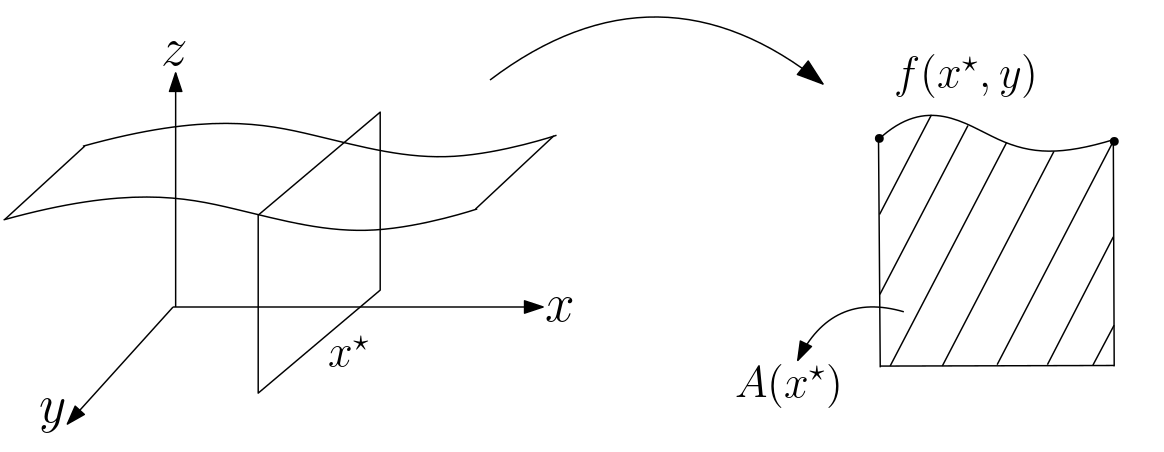
\includegraphics[width=0.8\linewidth]{MATH314_Notes_Fig5.png}
	   		 	   		 	\captionsetup{margin=1cm, justification=raggedright}\caption{\textbf{a)}Three dimensional interpretation of a cross-sectional intersection with a body. \textbf{b)} Cross-sectional area at an arbitrary $x^{\star}$ .}
	   		 	   		 \end{figure}
	   		 His principle states that the volume of the body is $\int_{a}^{b} A(x) \  dx$. To see this we portion $[a,b]$ into $a=x_{0} < x_{1} < \dots < x_{n} =b$, which in return implies 
	   		 $$ \int_{a}^{b} A(x) \  dx \approxeq \sum_{i=0}^{n-1}\underbrace{A(c_{i})(x_{i+1}- x_{i})}_{\mathclap{\text{olume of each slab (Figure )}}}.$$
	   		 $A(x_{i})$ gives the cross-sectional area at some $c_{i} \in [x_{i} , x_{i+1}]$. Therefore adding each slab between $x_{i}$ and $x_{i+1}$ yields the approximate volume. Moreover, using \eqref{eq_double_integral} ,
	   		 $$ \text{If volume} \ = \int_{a}^{b}A(x) \ dx = \int_{a}^{b}\int_{c}^{d} f(x,y) \ dydx \implies A(x) =\int_{c}^{d} f(x,y) \ dy. $$
	   		 \begin{figure}[H]
	   		 	\centering
	   		 	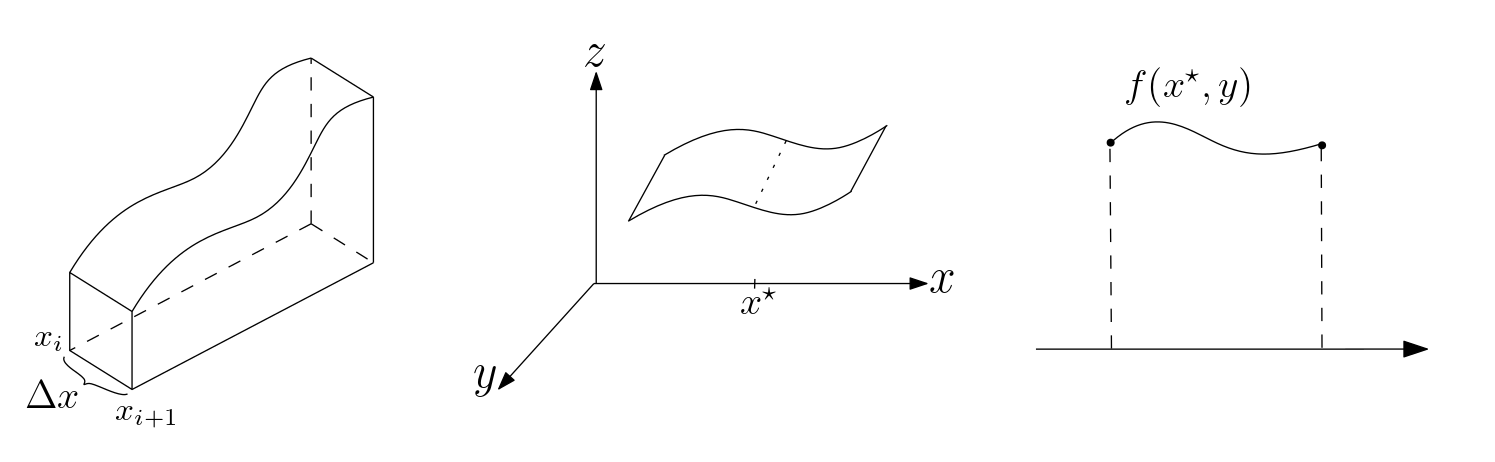
\includegraphics[width=\linewidth]{MATH314_Notes_Fig4.png}
	   		 	\captionsetup{margin=1cm, justification=raggedright}\caption{\textbf{a)}A slab of Reinmann sum partition. \textbf{b)} Setting an arbitrary $x^{\star}$ on a given plane \textbf{c)} The curve of the sliced function at $x^{\star}$.}
	   		 \end{figure}
	   		 But does this make sense ? Fix a $x^{\star}$, as shown in Figure ,then slicing at $x^{\star}$ we get the curve as illustrated in Figure. Clearly, $\int_{c}^{d}f(x^{\star},y) \ dy = A(x^{\star})$. Similarly, we can think of the volume as 
	   		 $$ \int_{c}^{d} A(y) \ dy  \quad \text{,where } \ A(y) = \int_{a}^{b}f(x,y) \ dx.$$
 	   		 To summarize, we have the following definition
 	   		 
	   		 \begin{definition}[Cavalier's Principle]
	   		 \label{def_cavalier_principle}
	   		 	Suppose a body has cross sectional area at $x$ given by $A(x)$, then the volume of the body is $\int_{a}^{b} A(x) \ dx$. Moreover ,
	   		 	\begin{equation} 
	   		 	\text{If volume }  = \int_{a}^{b} A(x) \ dx = \int_{a}^{b} \int_{c}^{d} f(x,y) \ dydx \implies A(x) = \int_{c}^{d} f(x,y) \ dy. \label{eq_cavalier}
	   		 	\end{equation}
	   		 	Similarly, we can think of the volume as 
	   		 	$$ \int_{c}^{d} A(y) \ dy , \qquad \text{where} \ \  A(y) = \int_{a}^{b} f(x,y) \ dx.$$
	   		 \end{definition}
	   		 
	   		 \begin{example}
	   		 	Use Cavalier's principle to compute the volume of a function $f(x) \ge 0$ defined for $x\in [a,b]$ rotated about the x-axis.
	   		 	\begin{figure}[H]
	   		 		   		 		\centering
	   		 		   		 		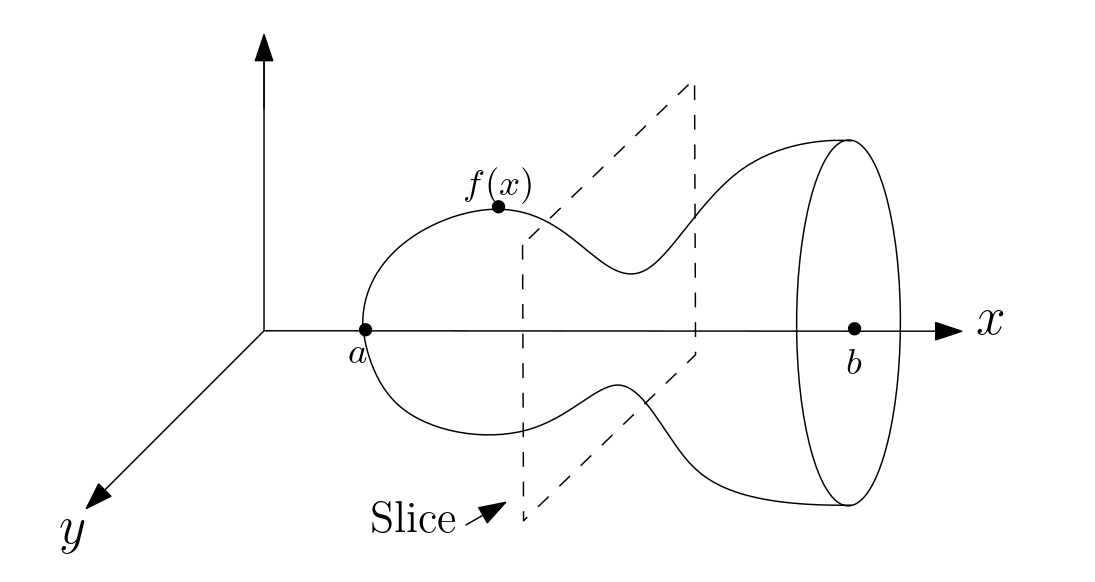
\includegraphics[width=0.5\linewidth]{MATH314_Notes_Double_Integral_Figure.png}
	   		 		   		 	\end{figure}
	   		 	If we look at this through $yz$ we in fact see a circle, therefore using $\eqref{eq_cavalier}$
	   		 	\begin{equation}
	   		 		A(x) = \pi(f(x))^{2} \implies V = \int_{a}^{b} \pi (f(x))^{2} \ dx.
	   		 	\end{equation}
	   		 \end{example}
	   		 
	   		 \begin{definition}
	   		 	If the sequence ${S_{n}}$ converges as $n\to \infty$ and the limit is the same regardless of the $c_{jk}$ chosen then $f$ is called integrable over $R$, with $$ \lim_{n \to \infty} \sum_{j,k = 0}^{n-1} f(c_{jk}) \Delta A = \int\limits_R f.$$
	   		 \end{definition}
	   		 
	   		 \begin{theorem}
	   		 	Let $f : R \subseteq \R^{2} \to \R $ be bounded on $R$ and suppose the set of points where $f$ is discontinuous comprises a finite union of graphs of continuous functions. In this situation , $f$ is integrable on $R$.
	   		 \end{theorem}
	   		 
	   		 \subsection{Properties of Integrable Functions}
	   		 \begin{enumerate}[label=(\roman*)]
	   		 	\item \textbf{Homogeneity} $\int\limits_R c f(x,y) \ dA = c \int\limits_R f(x,y) \ dA , \ c \in \R.$ 
	   		 	\item \textbf{Monotonicity } If $f(x,y) \ge g(x,y)$ , then $\int\limits_R f(x,y) \ dA \ge \int\limits_R g(x,y) \ dA.$ 
	   		 	\item \textbf{Additivity} If $R_{i} $ for $i =1 , \dots, n$ are disjoint rectangles, then $f$ is integrable for each $R_{i}$. Then if $Q= \bigcup\limits_{i=1} R_{i} = R_{1} \cup R_{2} \cup \dots \cup R_{n}$, then 
	   		 	\begin{equation} 
	   		 	\sum_{i=1}^{m} \int\limits_{R_{1}} f \ dA = \int\limits_Q f \ dA, 
	   		 	\end{equation}
	   		 	i.e., integrating rectangles individually on all is the same.
	   		 \end{enumerate}
	   		 
	   		 \begin{theorem}[Fubini's Theorem]
	   		 \label{thm_fubini}
	   		 	Let $f$ be a continuous function with domain $R = [a,b] \cross [c,d]$ , then
	   		 	\begin{equation} 
	   		 	\int_{a}^{b} \int_{c}^{d} f(x,y) \ dxdy = \int_{c}^{d} \int_{a}^{b} f(x,y) \ dy dx. \label{eq_fubini}
	   		 	\end{equation}
	   		 \end{theorem}
	   		 \begin{proof}
	   		 	Partition $[c,d]$ \ \ $c=y_{0} < y_{1} < \dots < y_{n} = d$. 
	   		 	\begin{gather*}
	   		 		\text{Let } \  F(x) = \int_{c}^{d}f(x,y) \ dy. \ \ 
	   		 		\implies F(x)= \sum_{k=0}^{n-1}\int_{y_{k}}^{y_{k+1}}f(x,y) \ dy \quad \text{(by additivity)}
	   		 	\end{gather*}
	   		 	\textbf{Recall:} The mean value theorem for integration, 
	   		 	$$ \int_{a}^{b} h (t)g(t) \ dt= h(c)\int_{a}^{b}g(t) \ dt \quad , c\in [a,b].$$
	   		 	\begin{align*}
	   		 		\implies \int_{y_{k}}^{y_{k+1}} f(x,y) \ dy &= f(x,y_{k}(x)) \int_{y_{k}}^{y_{k+1}} \ dy\\
	   		 		&= f(x,y_{k}(x))(y_{k+1}-y_{k}) \quad,y_{k(x)} \in [x_{k}, x_{k+1}]
	   		 	\end{align*}
	   		 	\begin{align*}
	   		 		&\therefore f(x) = \sum_{k=0}^{n-1}f(x,y_{k}(x))(y_{k+1}-y_{k}) \\
	   		 		\text{use } &\therefore \int_{a}^{b} F(x) \ dx = \lim\limits_{n\to\infty}\sum_{j=0}^{n-1}F(p_{j})(x_{j+1}-x_{j}),
	   		 		\intertext{where  $a = x_{0}< x_{1}<x_{2}<\dots < x_{n}=b$ and $p_{j}\in [x_{k},x_{k+1}]$.}
	   		 		&\text{set } c_{jk} = (p_{j}, y_{k}(p_{j})) \implies (p_{j}) = \sum_{k=0}^{n-1}f(c_{jk})(y_{k+1}-y_{k})
	   		 	\end{align*}
	   		 	\begin{align*}
	   		 		\therefore \int_{a}^{b}\int_{c}^{d}f(x,y) \ dydx = \int_{a}^{b} F(x) \ dx &= \lim\limits_{n\to \infty}\sum_{j=0}^{n-1} F(p_{j})(x_{k+1}-x_{k})\\
	   		 		&= \lim\limits_{n\to \infty}\underbrace{\sum_{j=0}^{n-1} \sum_{k=0}^{n-1}f(c_{jk})(y_{k+1}-y_{k})(x_{k+1}-x_{k})}_{\mathclap{\text{Rienmann sum for $\int\limits_{R} f \ dA$.}}}\\
	   		 		&= \int\limits_{R} f(x,y) \ dA. 
	   		 	\end{align*}
\	   		 \end{proof}
	   		 
	   		 \begin{example}
	   		 	Use Fubini's theorem $\eqref{thm_fubini}$ to show that 
	   		 	$$ \int_{0}^{1} \int_{0}^{2} x^{2}+y \ dy dx = \int_{0}^{2}\int_{0}^{1} x^{2}+y \ dx dy.$$
	   		 	\begin{gather*}
	   		 		\int_{0}^{1} \eval{x^{2}y + \frac{y^{2}}{2} }_{0}^{2} \ dx = \int_{0}^{1} 2x^{2}+ 2x \ dx = \eval{\frac{2x^{3}}{3} + 2x}_{0}^{1} = \frac83 .\\
	   		 		\int_{0}^{2}\int_{0}^{1} x^{2}+ y \ dx dy = \int_{0}^{2} \eval{\frac{y}{3} + \frac{y^{2}}{2}}_{0}^{2} = \frac83 .
	   		 	\end{gather*}
	   		 \end{example}
	   		 
	   		 \subsection{Integration Over More General Domain }
  			      Here we consider domain of integration where $x\in [a,b] , \phi_{1}(x) \le y \le \phi_{2}(x)$. Or similarly, $y\in [c,d] , \phi_{1}(y) \le x \le \phi_{2}(y)$. Suppose a region $D \subseteq \R$ defined by the previous domain of integration, can we say that 
  			      $$ \int_{a}^{b}\int_{\phi_{1}(x)}^{\phi_{2}(x)} f(x,y) \ dydx = \int_{c}^{d}\int_{\phi_{1}(y)}^{\phi_{2}(y)} f(x,y) \ dxdy ?$$
  			      To do this we use the more general form of Fubini's theorem.
  			  
  			\begin{theorem}[Fubini's Theorem Generalized]
  			\label{thm_fubini_generalized}
  				Let $f$ be a bounded function with domain $R = [a,b] \cross [c,d]$ and suppose the discontinuity of $f$ from a finite union of graphs of continuous functions. 
  				\begin{gather}
  					\text{Then if } \ \ \int_{c}^{d}f(x,y) \ dy \ \exists \ \forall \ x\in [a,b] \ \text{ and } \ \int_{a}^{b} f(x,y) \ dx \ \exists \ \forall \ y \in [c,d] ,\nonumber \\
  					\text{then } \ \int_{a}^{b}\int_{c}^{d}f(x,y) \ dydx = \int_{c}^{d}\int_{a}^{b}f(x,y) \ dxdy. 
   				\end{gather}
  			\end{theorem}
  			
  			\subsection{Triple Integrals}
  				Given a continuous function $f : B \to \R$ where $B$ is a rectangular parallelepiped in $\R^{3}$. We define the integral of $f$ over $B$ as 
  				$$ \lim_{n\to \infty}S_{n} \qquad \text{,where} \ \ S_{n} = \sum_{i=0}^{n-1}\sum_{j=0}^{n-1}\sum_{k=0}^{n-1} f(c_{ijk})\Delta V,$$
  				for which $c_{ijk}$ are some points in $B_{ijk}$.
  				
  			\begin{definition}
  				Let $f$ be a bounded function of $3$ variables defined on $B$. If $\lim\limits_{n\to \infty}S_{n}$ exists and is the same for any choice of $c_{ijk}$ , then $f$ is integrable  with 
  				\begin{equation} 
  				\lim\limits_{n\to \infty}S_{n} = \int\limits_B f \ dV = \iiint\limits_B f = \iiint f(x,y,z) \ dxdydz.
  				\end{equation}
  				
  				Moreover, from Fubini's theorem $\eqref{thm_fubini_generalized}$ since $f$ is continuous and $B = [a,b] \cross [c,d] \cross[u,v]$ then,
  				\begin{equation} 
  				\int\limits_B f \ dV = \int_{a}^{b} \int_{c}^{d}\int_{u}^{v} f(x,y,z) \ dzdydx = \int_{d}^{c} \int_{a}^{b} \int_{u}^{v} f \ dzdxdy = \dots \  \text{all combinations.}
  				\end{equation}
  			\end{definition}
  			 
  			 \noindent We can discuss integrability and switching order of integration on the domain \\$\omega := x\in [a,b] , \phi_{1}(x) \le y \le \phi_{2}(x), \phi_{1}(x,y) \le z \le \phi_{2}(x,y)$, by placing $\omega$ in a larger parallelepiped $B$ and using same ideas as in $\R^{2}$. 
  			 The volume of $\omega$ is given by $\iiint\limits_\omega 1 \ dV = \text{Volume}(\omega)$.
  			 Using the $\omega$ described above we have 
  			 \begin{gather*}
  			 	\int_{a}^{b} \int_{\phi_{1}(x)}^{\phi_{2}(x)} \int_{\phi_{1}(x,y)}^{\phi_{2}(x,y)} 1 \ dV = \underbrace{\int_{a}^{b} \int_{\phi_{1}(x)}^{\phi_{2}(x)} \phi_{2}(x,y) - \phi_{1}(x,y) \ dydx}_{\text{Double integral, i.e., volume below $\phi_{2}$ and above $\phi_{1}$}}.
  			 \end{gather*}
	  			 \begin{figure}[H]
  			 		\centering
  			 		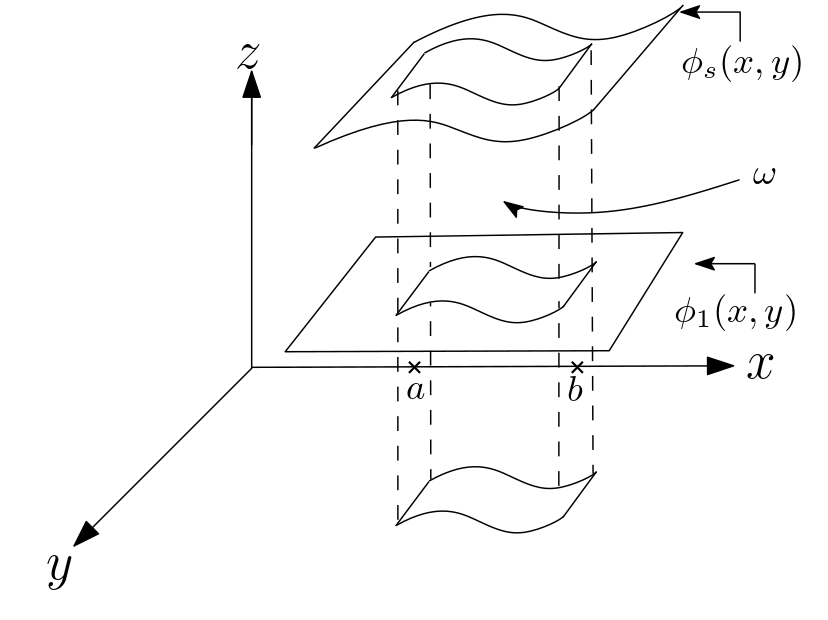
\includegraphics[width=0.5\linewidth]{MATH314_Notes_Triple_Integral_Figure.png}
  			 		\captionsetup{margin=1cm, justification=raggedright}\caption{Volume $\omega$ of an extended paralleled for triple integral integration.}
  			 \end{figure}
  			
  			\begin{example}
  				Compute the volume of the unit sphere.
  				
  				\noindent Sketch the graphs and deduce that we must set $\phi_{2}(x,y) = - \sqrt{1 - x^{2} - y^{2}}$ , $\phi_{1}(x,y) = \sqrt{1-x^{2} - y^{2}}$ , $\phi_{1}(x) = - \sqrt{1- x^{2}}$ and finally $\phi_{2}(x) = \sqrt{1-x^{2}}$. So we have 
  				\begin{gather*}
  					\int_{-1}^{1} \int_{-\sqrt{1-x^{2}}}^{\sqrt{1-x^{2}}}\int_{-\sqrt{1-x^{2}-y^{2}}}^{\sqrt{1-x^{2}-y^{2}}} 1 \ dzdydx = 2 	\int_{-1}^{1} \int_{-\sqrt{1-x^{2}}}^{\sqrt{1-x^{2}}} \sqrt{1-x^{2} - y^{2}} \ dydx. \\
  					\int_{-\sqrt{1-x^{2}}}^{\sqrt{1-x^{2}}} \sqrt{(1-x^{2}) - y^{2}} \ dy , \quad \text{let } \ u = \sqrt{1-x^{2}}, \ \ \int_{-a}^{a} \sqrt{a^{2} - y^{2}} \ dy
  			 	\end{gather*}
  			 	let $y = \cos \theta$ and $dy/d\theta  = - \sin \theta$ , so then 
  			 	\begin{align*}
  			 		\int \sqrt{a^{2} - x^{2}} \ dy &= -a \int \sin \theta \sqrt{a^{2} - x^{2}\cos^{2}\theta} \ \d\theta  = -a^{2}\int \sin^{2} \theta  \\
  			 		&= -a^{2}\int \frac{1-\cos(2\theta)}{2} \ d\theta = \frac{-a^{2}\theta}{2} + \frac{\sin(2\theta) a^{2}}{4} + C.
  			 		\intertext{Using $\sin(2\theta) = 2\sin\theta \cos \theta $ we get }
  			 		&= -a^{2} \left(\frac{\arccos(\sfrac{y}{a})}{2}\right) + \frac{a}{2}y \sin \theta + C 
  			 	\end{align*}
  			 	$\sin\theta  = \frac{\sqrt{a^{2} - y^{2}}}{2}$ so we may write the result 
  			 	\begin{gather*}
  			 		= \frac{-a^{2}}{2} \arccos(1) + \frac{a^{2}}{2} \arccos (-1) = \frac{a^{2}}{2}\pi \\
  			 		\therefore \text{the volume is : } \int_{-1}^{1} \frac{(1-x^{2})\pi}{2} \ dx = \frac{4\pi}{3} .
  			 	\end{gather*}
  			 	
  			\end{example}
  			 
  			\begin{example}
  				Find an integral for the volume of the region enclosed by the paraboloid \newline  $z=x^{2} + y^{2}$ and the plane $z= 3- 2y$
  				\begin{figure}[H]
  					\centering
  					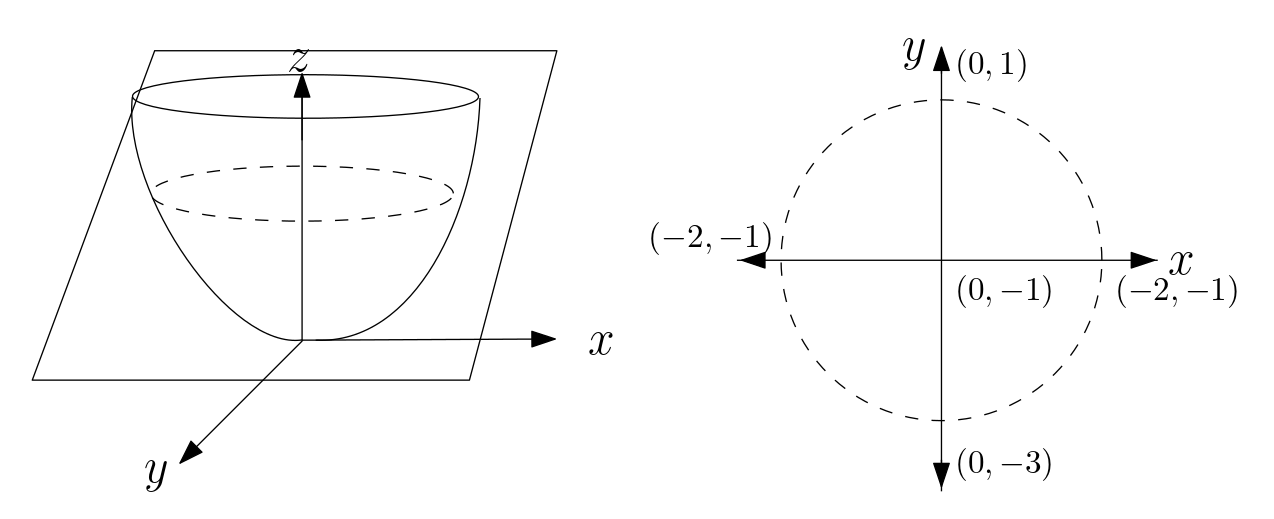
\includegraphics[width=0.75\linewidth]{MATH314_Notes_Triple_Integral_Example1_Figure.png}
  					\captionsetup{margin=1cm, justification=raggedright}\caption{Figure associated with the current example. \textbf{a)} The given plane intersect the paraboloid. \textbf{b)} An elevated view of the intersection along with coordinates are provided.}
  				\end{figure}
  				\noindent From the figure we have to deduce that $z$ is bounded as $x^{2}+y^{2} \le z \le 3-2y$. Now we need either $x\in [a,b] , \phi_{1}(x)\le y \le \phi_{2}(x)$ or $y \in [c,d] , \phi_{1}(y) \le x \le \phi_{2}(y)$. 
  				The surfaces intersect along the curve given by $x^{2}+y^{2} = 3-2y \implies x^{2} + y^{2} + 2y =3. $ This is in fact a circle of radius $2$ shifted down since $x^{2} + y^{2} + 2y +1 -1 = 3 \equiv x^{2} + (y+1)^{2} =4 ! $
  				
  				\noindent And so we have $-\sqrt{4-(y+1)^{2}} \le x \le \sqrt{4-(y+1)^{2}} , y\in [-3,1]$.
  				$$ \therefore \text{Volume is given by } \ \int_{-3}^{1} \int_{-\sqrt{4-(y+1)^{2}}}^{\sqrt{4-(y+1)^{2}}}\int_{x^{2}+y^{2}}^{3-2y} dzdxdy.$$
  			\end{example}
  			
  			\subsection{Change of Variables Coordinates}
  			
  			\begin{theorem}
  				Let $A$ be a $2\cross 2$ matrix and suppose $T: \R^{2} \to \R^{2}$ is given by $T(\vec{x}) = A \vec{x}$, then $T$ maps parallelograms to parallelograms.
  			\end{theorem}
  			
  			\begin{example}
  				Consider $T(x,y) = ((x+y)/2 , (x-y)/2)$
  				$$ T(x,y) = 
  				\begin{bmatrix}
  					1/2 & 1/2 \\
  					1/2 & -1/2 
  				\end{bmatrix}
  				\begin{bmatrix}
  					\vphantom{1/2}	x \\
  					\vphantom{1/2}y
  				\end{bmatrix}$$
  				$T$ maps paral. to paral.
  				%TODO complete this shit
  			\end{example}
  			
  			\noindent How do we apply this to integration ? Consider $\iint\limits_D f(x,y)\ dA $ and let $T: (u,v) \to (x(u,v), y(u,v))$.
  			\begin{align*}
  				&\bullet \text{The point in the xy-plane can be given by points in the uv-plane through $T$.} \\
  				&\bullet T(u,v) = (x(u,v), y(u,v)).
  			\end{align*}
  			Near a point $(u_{0} , v_{0})$ we have,
  			$$T(u,v) \approx T(u_{0}, v_{0}) + DT(u_{0},v_{0})
  			\begin{bmatrix}
  				u-u_{0}\\
  				v-v_{0}
  			\end{bmatrix},$$
  			where $DT(u_{0} , v_{0})$ is the Jacobian. Near $(u_{0}, v_{0})$,
  			\begin{equation} 
  			T(u,v) \approx T(u_{0},v_{0}) + 
  			\eval{\begin{bmatrix}
  				\pdv{x}{u} & \pdv{x}{v} \\
  				\pdv{y}{u} & \pdv{y}{v}
  			\end{bmatrix}}_{(u_{0},v_{0})}
  			\begin{bmatrix}
  					\vphantom{\pdv{x}{u}}(u-u_{0})\\ 	\vphantom{\pdv{x}{u}}(v- v_{0})
  			\end{bmatrix}.
  			\end{equation}
  			Note that this is a linear transformation with $T = A\vec{x} \implies T$ sends parallelograms to parallelograms. Through some algebraic manipulations that we will omit in this manuscript, we obtain the following important result 
  			\begin{equation} 
  			\iint\limits_D f(x,y) \ dxdy = \iint\limits_S f(u,v) \abs{\frac{\partial (x,y)}{\partial (u,v)}} \ dudv , \label{eq_mapping_term_integral}
  			\end{equation}
  			where $S$ is the domain $D$ in the $uv$ coordinate system, also called \textit{the description of $D$}.
  			
  			\begin{example}
  				$$ \text{Solve } \ \int_{-1}^{1}\int_{-\sqrt{1-y^{2}}}^{\sqrt{1-y^{2}}} \ dxdy.$$
  				Set $x = r \cos \theta$ and $y = r \sin \theta$. Recalling \eqref{eq_mapping_term_integral}
  				\begin{gather*}
  					\implies \abs{\frac{\partial (x,y)}{\partial (r,\theta )}} = \abs{\det 
  					\begin{vmatrix}
  						\cos \theta & -r\sin \theta \\
  						\sin \theta & r\cos \theta 
  					\end{vmatrix}
  					} =r \\
  					\implies = \iint\limits_S r \ drd\theta \ \text{where $S$ is the unit circle in polar coordinates} \\
	  					= \int_{0}^{2\pi } \int_{0}^{1} r \ drd\theta  = \int_{0}^{2\pi} \eval{\frac{r^{2}}{2}}_{0}^{1} \ d\theta = \pi.
  				\end{gather*}
  			\end{example}
  			
  			\begin{example} 
  			$$ \text{Compute } \ \iint\limits_R e^{\frac{x+y}{x-y}} \ dA,$$
  			where $R$ is the trapezoid with vertices $(1,0) , (2,0) , (0,-1), (0,-2).$ 
  			Try $u = x+y$ with $v = x-y$. $x = u-y \implies v = (u-y)-y \implies 2y = u-v \implies y= \frac{u-v}{2}$ and $x=\frac{u+v}{2}$
  				\begin{figure}[H]
  					\centering
  					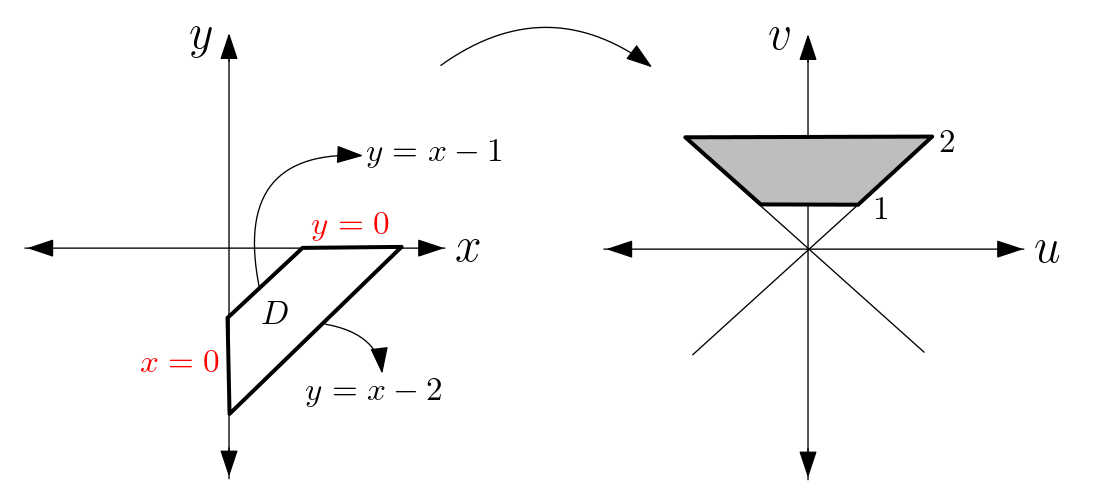
\includegraphics[width=0.75\linewidth]{MATH314_Notes_Triple_Integral_Example2_Figure.png}\captionsetup{margin=1cm, justification=raggedright}\caption{Figure for the current example.\textbf{a)} The original trapezoid. \textbf{b)} The transformed trapezoid.}
  				\end{figure}
  			\noindent From a) and b), we have that $y=0 \implies u=v$ and $x=0 \implies u=-v$. From $u = x+y$ and $v=x-y$ we get $y = x-1 \implies v=1$ and $y = x-2 \implies v=2$.
  			
  			\noindent Now how do we integrate over b)? 
  			\begin{gather*}
  				\int_{1}^{2}\int_{-v}^{v} e^{\sfrac{u}{v}} \abs{\frac{\partial (x,y)}{\partial (u,v)}} \ dudv  \ \to \
  				\abs{\frac{\partial (x,y)}{\partial (u,v)}} = \abs{\det 
  				\begin{vmatrix}
  					1/2 & 1/2 \\
  					1/2 & -1/2
  				\end{vmatrix}
  				} =\frac12 
  			\end{gather*}
  			\begin{align*}
  				\implies \int_{1}^{2}\int_{-v}^{v} e^{\frac{u}{v}} \ dudv 
  				  				&= \frac12 \int_{1}^{2} \eval{ve^{\sfrac{u}{v}}}_{-v}^{v} \ dv = \frac12 \int_{1}^{2} v \left(e^{\sfrac{v}{v}} - e^{\sfrac{-v}{v}}\right) \ dv \\
  				  				&= \frac12 \left(e^{1} - e^{-1}\right) \int_{1}^{2} v \ dv = \frac12 (e^{1} - e^{-1})(2- \frac12) = \frac34 (e-e^{-1}).
  			\end{align*}
  			\end{example}
  			
  			\rule{\linewidth}{0.4 pt}
  		
  		\noindent Last time we introduced change of coordinates for double integrals 
  		$$ \iint\limits_D f(x,y) \ dxdy = \iint\limits_S f(x(u,v) ,y(u,v)) \abs{\frac{\partial (x,y)}{\partial (u,v)}} \ dudv ,$$
  		where $S$ is the description of $D$ in the uv-plane.
  		\\
  		\noindent The same thing holds for triple integrals, when integrating functions $f: \R^{3} \to \R$. Suppose $f(x,y,z) = f(x(u,v,w) , y(u,v,w) , z(u,v,w))$ (change of coordinates), then we have 
  		\begin{gather}
  			T(u,v,w) \approx T(u_{0},v_{0},w_{0}) + 
  			\eval{\begin{bmatrix}
  				\pdv{x}{u} & \pdv{x}{v} & \pdv{x}{w} &\\
  				\pdv{y}{u} & \pdv{y}{v} & \pdv{y}{w} &\\
  				\pdv{z}{u} & \pdv{z}{v} & \pdv{z}{w} &\\
  			\end{bmatrix}}_{(u_{0},v_{0},w_{0})} 
  			\begin{bmatrix}
  				\vphantom{\pdv{x}{u}}u-u_{0}\\
  				\vphantom{\pdv{x}{u}}v-v_{0} \\
  				\vphantom{\pdv{x}{u}}	w-w_{0}
  			\end{bmatrix}.
  		\end{gather}
  		Using the same argument as before we get,
  		\begin{equation} 
  		\iiint\limits_D f(x,y,z) \ dxdydz = \iiint\limits_S f(y,v,w) \abs{\frac{\partial(x,y,z)}{\partial (u,v,w)}} \ dudvdw.
  		\end{equation}
  		\subsection{Cylindrical Coordinates}
  			The following transformations are done in the cylindrical coordinates 
  			\begin{equation*}
  				\begin{rcases}
  					x &= r \cos \theta \\
  					y &=  r \sin \theta \\ 
  					z &= z
  				\end{rcases} \implies \frac{\partial (x,y,z)}{\partial (r,\theta, z)} = \det 
  				\begin{vmatrix}
  					\cos \theta & -r \sin \theta & 0 \\
  					\sin \theta & r\cos \theta & 0 \\
  					0 & 0 & 1
  				\end{vmatrix} = r.
  				\label{eq_cylindrical_coord}
  			\end{equation*}
  		
  		\begin{example}
  			Find the volume enclosed by the paraboloid $z=x^{2}+y^{2}$ and the plane $z=3-2y$, same example as seen before.
  			$$ \int_{1}^{3}\int_{-\sqrt{3-2y-y^{2}}}^{\sqrt{3-2y-y^{2}}}\int_{x^{2}+y^{2}}^{3-2y} \ dzdxdy,$$
  			Let us translate this into cylindrical coordinates.
  			Recall that we said the intersection circle is a shifted by -1 , with radius $2$ and is overall described by $x^{2} + (y+1 )^{2} = 4.$ Now let us set $x= r\cos \theta , y= -1 + r\sin\theta$ and $z=z$. This is a \textit{shifted cylinder}. 
  			\begin{align*}
  				x^{2}+y^{2} &= r^{2} \cos^{2}\theta +(r\sin\theta-1)^{2} \\
  				&= r^{2}\cos^{2}\theta + r^{2}\sin^{2}\theta +2 r \sin \theta +1  = r^{2} - 2r\sin \theta +1.
  				\intertext{Also, $3-2y = 3-2(r\sin\theta -1 ) = 5-2r\sin\theta$}
  			\end{align*}
  			Having transformed the given structures , we may solve the triple integral 
  			\begin{align*}
  				=\int_{0}^{2\pi } \int_{0}^{2} \int_{r^{2}-2r\sin\theta +1 }^{5-2r \sin\theta }  r \ dzdr d\theta &= \int_{0}^{2\pi} \int_{0}^{2} ((t-2r\sin \theta) - (r^{2}-2r\sin\theta  + 1)) r \ drd\theta \\
  				&= \int_{0}^{2\pi} \int_{0}^{2} (4-r^{2})r \ dr d\theta = (\dots ) = 8\pi.
  			\end{align*}
  		\end{example}
  		
  		\begin{example}
  			Find the volume of the region below $z= x+2$ and between $x^{2} + y^{2} = 1$ and $x^{2} + y^{2} = 4$. Sketching these constraints we get a region defined between a circle of radius $1$ a circle of radius $2$. We may immediately solve the problem ,
  			$$ \int_{0}^{2\pi} \int_{1}^{2} \int_{0}^{r\cos \theta +z} r \ dzdrd\theta = \int_{0}^{2\pi} \int_{1}^{2} r^{2} \cos \theta + 2r \ dr d\theta = \int_{0}^{2\pi}\eval{\frac{r^{3}}{3} \cos \theta +r^{3}}_{1}^{2} \ d\theta = (\dots )= 6\pi.$$
  		\end{example}
  		
  		\subsection{Spherical Coordinates}
  		For spherical coordinates we have the following transformations 
  		\begin{align*}
  			&\bullet x = \rho \sin \vphi \cos \theta \\
  			&\bullet y = \rho \sin \vphi \sin \theta \\
  			& \bullet z = \rho \cos \vphi.
  		\end{align*}
  		
  		\begin{figure}[H]
  			\centering
  			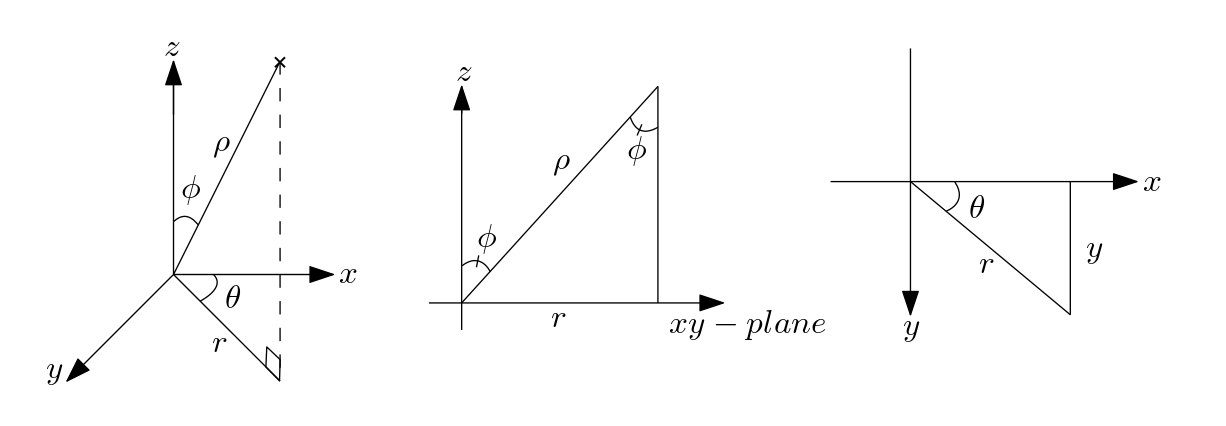
\includegraphics[width= 0.8\linewidth]{MATH314_Notes_Triple_Integral_Example3_Figure.png}
  			\captionsetup{margin=1cm, justification=raggedright}\caption{Three perspectives of the spherical coordinates. Important notes include that $\rho$ is the distance from the origin, $\theta$ is the angle between the positive $x$-axis and the vector $(x,y,0)$, $(0\le \theta \le 2\pi)$. Finally, $\phi$ is the angle between the positive $z$-axis and the vector $(x,y,z)$, $(0 \le \phi \le \pi)$.}
  		\end{figure}
  		Let us determine the corresponding Jacobian to spherical coordinates transformation. 
  		\begin{equation*}
  			\frac{\partial (x,y,z)}{\partial (\rho, \theta, \vphi)}  = 
  			\det\begin{vmatrix}
  				\sin\vphi \cos \theta & -\rho \sin \vphi \sin \theta & \rho \cos \vphi \cos \theta \\
  				\sin\vphi \sin \theta & \rho \sin \vphi \sin \theta & \rho \cos \vphi \sin \theta \\
  				\cos \vphi & 0 & -\rho \sin \vphi
  			\end{vmatrix}
  		\end{equation*}
  		\begin{align*}
  			&= \rho^{2} \cos \vphi (-\sin\vphi \cos \phi \sin ^{2}\theta - \sin \vphi\cos \vphi \cos^{2}\theta )- \rho^{2}\sin \vphi(\sin^{2}\vphi \cos^{2} \theta + \sin \vphi \sin^{2 }\theta) \\
  			&= -\rho^{2}\cos^{2} \vphi \sin \vphi - \rho^{2}\sin^{3}\vphi = \boxed{-\rho^{2}\sin \vphi} .
  		\end{align*}
  		
  		\begin{example}
  			Compute the volume of the sphere of radius $r$ in spherical coordinates.
  			The squelet of a spherical integral is 
  			$$\int\limits_{\vphi} \int\limits_{\theta}\int\limits_{\rho} \rho^{2} \sin \vphi \ d\vphi d\theta d\rho.$$
  			So we have 
  			\begin{align*}
  				\int_{0}^{\pi} \int_{0}^{2\pi} \int_{0}^{r} \rho^{2}\sin \vphi \ d\vphi d\theta d \rho &= \int_{0}^{\pi} \int_{0}^{2\pi} \eval{\frac{\rho^{3}}{3} \sin \vphi}_{0}^{r} \ d\theta d \vphi \\
  				&=\int_{0}^{\pi}\int_{0}^{2\pi} \frac{r^{2}}{3}\sin \vphi \ d\theta d \vphi \\
  				&= \int_{0}^{\pi} \frac{2\pi r^{3}}{3} \sin \vphi \ d\vphi = (\dots ) = \frac{4\pi r^{3}}{3}.
  			\end{align*}
  		\end{example}

  		\begin{example}
  			Find the volume of the region above the cone $z=\sqrt{x^{2}+y^{2}}$ and below the unit sphere. Sketching these constraints gives us an upside down cone , with a semi-sphere sitting on top of it. Which coordinates should we use ?
  			
  			\begin{note}
  				For problems involving spheres and especially cones, spherical coordinates are appropriate.
  			\end{note}
  			
  			\noindent Let us find $(\vphi, \theta, \rho)$. We're looking for the intersection of the cone and the unit sphere which implies that $\rho =1.$ Express the given functions as $z^{2} = x^{2} + y^{2} \ \ \text{(cone)}$ and $z^{2} = 1-x^{2} - y^{2} \ \ (\text{(Sphere)})$. 
  			$$ \text{Equate these : } \xrightarrow{} x^{2}+ y^{2} =1 -x^{2} - y^{2} \implies z(x^{2} + y^{2}) =1 .$$
  			Now we go to the spherical coordinates, 
  			\begin{equation*}
  				\begin{rcases}
  					x &= \rho \sin \vphi \cos \theta \\
  					y &= \rho \sin \vphi \sin \theta \\
  					z &= \rho \cos \vphi
  				\end{rcases} \ \implies  \ 
  				\begin{align}
  					x^{2} + y^{2} &= \rho^{2} \sin \vphi \cos^{2}\theta + \rho^{2} \sin \vphi \sin^{2} \theta \\
  					&= \rho^{2} \sin^{2} \vphi (\cos^{2} \theta = \sin^{2}\theta) \\
  					&= \rho^{2}\sin^{2}\theta.
  				\end{align}
  			\end{equation*}
  			\begin{align*}
  				&\implies z\rho^{2}\sin^{2}\vphi = 1 ,\quad \text{with } \ \ \rho^{2}=1 \\
  				&\implies z\sin^{2}\vphi =1 \implies \sin^{2}\vphi = \frac12 \implies \sin\vphi = \frac{1}{\sqrt{2}} \ \ \therefore \vphi = \frac{\pi}{4}.
  			\end{align*}
  			So we have $\vphi \in [0, \frac{\pi}{4}]$ , $\theta \in [0, 2\pi]$ , $\rho \in [0,1]$
  			$$ \therefore \ \text{Volume is } \ \ \int_{0}^{\sfrac{\pi}{4}} \int_{0}^{2\pi}\int_{0}^{1} \rho^{2}\sin\vphi \ d\rho d\theta d\vphi = (...).$$
  			Calculations for the above integral are omitted since they're trivial.
  			
  			\noindent Note that the problem here is done, since we're only asking to find the volume - the problem could be more complicated if we were asked to integrate over or under a function.
  		\end{example}
  		
  		\noindent The density of a region $R \subseteq \R^{3}$ is given by $\rho(x,y,z)$, then the mass of $R$ is given by 
  		\begin{equation}
  			m(R) = \iiint\limits_{R}\rho (x,y,z) \ dV ,\label{eq_mass_equation}
  		\end{equation}
  		with the center of mass defined as $(\bar{x}, \bar{y} , \bar{z}),$ where 
  		\begin{equation*}
  			\bar{x} = \frac{\iiint\limits_R x \rho (x,y,z) \ dV }{m(R)}, \quad \bar{y} = \frac{\iiint\limits_R y \rho (x,y,z) \ dV }{m(R)} ,\quad \bar{z} = (\dots).$$
  		\end{equation*} 
  		
  		\begin{example}
  			Find the center of mass for the previous example (Cone/sphere) for $\rho = 1 $(density). We know by rotational symmetry that $\bar{x} = \bar{y} = 0$, we therefore just need 
  			\begin{gather*}
  				\bar{z} = \frac{\iiint\limits_{R} z \ dV}{m(R)} = \frac{\int_{0}^{\sfrac{\pi}{4}} \int_{0}^{2\pi} \int_{0}^{1}\rho^{3} \cos \vphi \sin \vphi \ d\rho d\theta d\vphi}{m(R)} = (...) = \frac{\frac{\pi}{2} \int_{0}^{\sfrac{\pi}{4}} \cos \vphi \sin \vphi \ d\vphi } {m(R)}.
  			\end{gather*}
  			\begin{equation*}
  				\cos \vphi \sin \vphi = \frac{\sin(2\vphi)}{2} \implies \bar{z} = \frac{\frac{\pi}{4} \int_{0}^{\sfrac{\pi}{4}} \sin (2\vphi) \ d\vphi}{m(R)} = \frac{\frac{\pi}{8} \big[-\cos(2(\sfrac{\pi}{4})) + \cos(0)\big]}{\frac{2\pi}{3} \big[1- \frac{1}{1\sqrt{2}}\big]} = \frac{3}{16(1- 1/\sqrt{2})}.
  			\end{equation*}
  			$$ \therefore \text{Center of mass is } \left(0,0, \frac{3}{16\left(1-\frac{1}{\sqrt{2}}\right)}\right).$$
  		\end{example}
  		
  		\newpage
  		\section{Line Integrals and Path Integrals}
  			
  			\begin{definition}[Path Integral]
  			\label{def_path_integral}
  				The path integral , or integral of $f(x,y,z)$ along the curve $\vec{\sigma}$, is defined when $\vec{\sigma} : [a,b] \to \R^{3}$ is continuous and differentiable on $[a,b]$ and when $f(\vec{\sigma}(t)) : t \to f(x(t), y(t) ,z(t))$ is continuous on $[a,b]$. The integral is defined as 
  				\begin{equation}
  					\int\limits_{\vec{\sigma}} f \ ds = \int_{a}^{b} f(x(t) , y(t) ,z(t)) \norm{\vec{\sigma}'(t)} \ dt = \int_{a}^{b} f(\vec{\sigma}(t)) \norm{\vec{\sigma}(t)} \ dt. \label{eq_path_integral}
  				\end{equation}
  			\end{definition}
  			
  			\begin{note}
  				If $f:= 1$ , then this gives the arclength of $\vec{\sigma}$ between $a$ and $b$.
  			\end{note}
  			
  			\begin{example}
  				Evaluate $\int\limits_{\vec{\sigma}}$ , where $\sigma$ consists of $\sigma_{1}$ which is the arc of a parabola $"(y = x^{2})"$ from $(0,0)$ to $(1,1)$. And, $\sqrt{2}$ is a function $(1,1) \to (1,2)$.
  				$$ \implies \int\limits_{\sigma} 2x \ dx =\int\limits_{\sigma_{1}} 2x \ dx+ \int\limits_{\sigma_{2}} 2x \ dx .$$
  				
  				Let us parameterize the functions and express what we're looking for . We want ,
  				\begin{align*}
  					\raggedright
  					& \sigma_{1} : t \to \R^{2} \\
  					& \vec{\sigma_{1}}(t) : \la t, t^{2} \ra \ \ t\in [0,1] \\
  					& \vec{\sigma_{2}}(t) : \la 1 , t\ra \ \  t\in [1,2]
  				\end{align*}
  				Let us find the first integral and second,
  				\begin{equation*}
  					\int\limits_{\vec{\sigma_{1}}} 2x \ dx = \int_{a}^{b} f(x(t), y(t)) \norm{\vec{\sigma_{1}}'(t)} \ dt \quad 
  					\begin{cases}
  						& x(t) =t \quad , y(t) = t^{2} \\
  						& \norm{\vec{\sigma_{1}}'(t)} = \sqrt{(x'(t))^{2} +(y'(t))^{2}}
  					\end{cases}
  				\end{equation*}
  				\begin{equation*}
  					\therefore \int\limits_{\vec{\sigma_{1}}} 2x \ dx = \int_{0}^{1} 2t \sqrt{1 + 4t^{2}} \ dt \stackrel{u = 1+4t^{2}}{=} \frac14 \int_{1}^{5} \sqrt{u} \ du = (\dots) = \left(\frac{5\sqrt{5} -1}{6}\right).
  				\end{equation*}
  				\begin{equation*}
	  				\text{For } \ \ \int\limits_{\vec{\sigma_{2}}} 2x \ dx = \int_{1}^{2} 2 \sqrt{1} \ dt = 2.\qquad \therefore \text{Path integral is} \ \boxed{\frac{5\sqrt{5}-1}{6} +2}.
  				\end{equation*}
  			\end{example}
  			
  			\begin{definition}[Vector Field]
  				A vector field $F$ on $\R^{n}$ is a map $F:U \subset \R^{n} \to \R^{n}$ that assigns to each point $\vec{x} \in U$ a vector $\vec{F}(\vec{x})$ . 
  				
  				For example, oxygen in a room , or any other quantity that is subjected to some forces inside a dimensional space.
  			\end{definition}
  			
  			\begin{definition}[Flow line]
  				If $\vec{F}$ is a vector field, a flow line for $\vec{F}$ is a path $\vec{\sigma}(t)$ such that $\vec{\sigma}'(t) = \vec{F}(\vec{\sigma}(t))$. 
  				
  				This can be extended to 
  				\begin{equation*}
	  				\begin{rcases}
	  					\dv{}{t}\sigma (\vec{x} ,t) &= F(\vec{\sigma} (\vec{x}(t))) \\
	  					\sigma(\vec{x} ,0) &= \vec{x} 
	  				\end{rcases}
	  				 \quad \text{The flowline with initial condition at $\vec{x}$ when $t=0$.}
  				\end{equation*}
  			\end{definition}
  			
  			\subsection{Divergence and Curl}
  				Let $\vec{F}$ be continuously differentiable with 
  				\begin{equation}
  					\vec{F}(\vec{x}) = \la F_{1}(\vec{x}) , F_{2}(\vec{x}), F_{3} (\vec{x}) \ra = F_{1}(\vec{x})\vec{i} + F_{2})(\vec{x})\vec{j} + F_{3}(\vec{x})\vec{k}.\label{eq_curl_vector}
  				\end{equation}
  				\begin{gather}
  					\text{ The Curl of } F  = \nabla \cross \vec{F} = \det
  					\begin{vmatrix}
  						\hat{i} & \hat{j} & \hat{k} \\
  						\pdv{}{x} & \pdv{}{y} &\pdv{}{z}\\
  						F_{1} & F_{2} & F_{3}
  					\end{vmatrix} \label{eq_curl_matrix}\\
  					\implies \text{Curl}(\vec{F}) = \left(\pdv{F_{3}}{y} - \pdv{F_{2}}{z}\right)\vec{i} +\left(\pdv{F_{1}}{z} - \pdv{F_{3}}{x}\right)\vec{j} +\left(\pdv{F_{2}}{x} - \pdv{F_{1}}{y}\right)\vec{k} \label{eq_curl_parantheses}. 
  				\end{gather}
  				The curl describes the rotation of a vector field. The curl of $\vec{F}$ of $\vec{x}$ yields a vector pointing along the axis of rotation where the length $\norm{\nabla \cross F}$ describes the magnitude of the rotation.
  				
  				\begin{theorem}
  					If $f$ is twice continuously differentiable $(C^{2})$  then $\nabla \cross (\nabla f) =0 $ , (where $f$ is scalar-valued)
  				\end{theorem}
  				
  				\begin{definition}[Conservative]
  					A vector field is called conservative if $F= \nabla f$ , for some real-valued function $f$, implying that the curl of any conservative vector field is $0$.
  				\end{definition}
  				
  				\begin{example}
  					Determine if $f(x,y,z) = y^{2}z^{3}\vec{i} + 3xyz^{3}\vec{j} + 3x^{2}z^{2}\vec{k}$ is conservative. Using \eqref{eq_curl_parantheses}, 
  					\begin{align*}
	  					\text{curl}(F) &= (f_{3y} - f_{2z})\vec{i} + (f_{1z} - f_{3x})\vec{j} + (f_{2x} - f_{1y})\vec{k} \\
	  					&= (6xyz^{2} - 6xyz^{2})\vec{i} + (3y^{2}z^{2} - 3y^{2} z^{2})\vec{j} + (2yz^{3}-2yz^{2})\vec{k} \\
	  					&= \vec{0 }\ \ \ \therefore F \ \text{is conservative  (by Definition 8.4)}
  					\end{align*}
  				\end{example}
  				
  				\begin{definition}[Divergence]
  					The divergence of a continuously differentiable vector field $F$ is
  					 \begin{equation} 
  					  \nabla \cdot \vec{F} = \nabla \cdot \la F_{1} , F_{2} , F_{3} \ra = \pdv{F_{1}}{x} + \pdv{F_{2}}{y} + \pdv{F_{3}}{z}.
  					  \end{equation}
  				\end{definition}
  				
  				\begin{example}
  					Compute the Div$(\nabla f)$ , where $f: \R^{3} \to \R$
  					\begin{align*}
  						&= \left(\pdv{}{x}, \pdv{}{y}, \pdv{}{z}\right) , \left(\pdv{f}{x} , \pdv{f}{y} , \pdv{f}{z}\right) \\
  						&= \pdv{f}{x^{2}} + \pdv[2]{f}{z} + \pdv[2]{f}{z} = \nabla^{2} f = \Delta f
  					\end{align*}
  				\end{example}
  				
  				\begin{note}
  					$\nabla^{2} = \Delta$ is called the Laplace operator. For example, the heat equation ${\sfrac{\partial}{\partial t}(u(x,t) = \Delta u)}.$
  				\end{note}
  				
  				\noindent What does div $\vec{F}$ represent? Recall that the flow line $\vec{\sigma}$ starting at point $\vec{x}$ flowing under a vector field $\vec{F}$ is defined by 
  				\begin{equation*}
  					\begin{cases}
  						&\pdv{}{t} \vec{\sigma}(\vec{x},t) = F (\vec{\sigma}(\vec{x},t)) \qquad\quad (\star) \\
  						&\vec{\sigma}(\vec{x},0) =\vec{x}= (x_{1},x_{2},x_{3})
  					\end{cases} \ \ 
  					\begin{align*}
  						&\text{where } \ \sigma : \R^{3+1} \to \R \\
  						&\text{and} \ F:\R^{3} \to \R^{3} \ \text{with } F(\vec{x}) = (F_{1}(\vec{x}) , F_{2}(\vec{x}), F_{3} (\vec{x})).
  					\end{align*}
  				\end{equation*}
  				\noindent Let us differentiate $(\star)$ in $\vec{x}$, we get 
  				$$ \underbrace{D\vec{x} \pdv{}{t}\vec{\sigma}(\vec{x},t)}_{\text{Matrix}} = \underbrace{D\vec{x}F(\vec{\sigma}(\vec{x},t))}_{\text{Matrix}} \ \underbrace{D\vec{x}\vec{\sigma}(\vec{x},t)}_{\text{Matrix}} \quad \text{(by chain rule)}.$$
  				
  				\noindent Now consider the $3$ vectors $\vec{v_{1}} = \epsilon \vec{i} , \ \vec{v_{2}} = \epsilon \vec{j} , \ \vec{v_{3}}=\epsilon \vec{k}$ for some $\epsilon > 0.$
  				\begin{figure}[H]
  					\centering
  					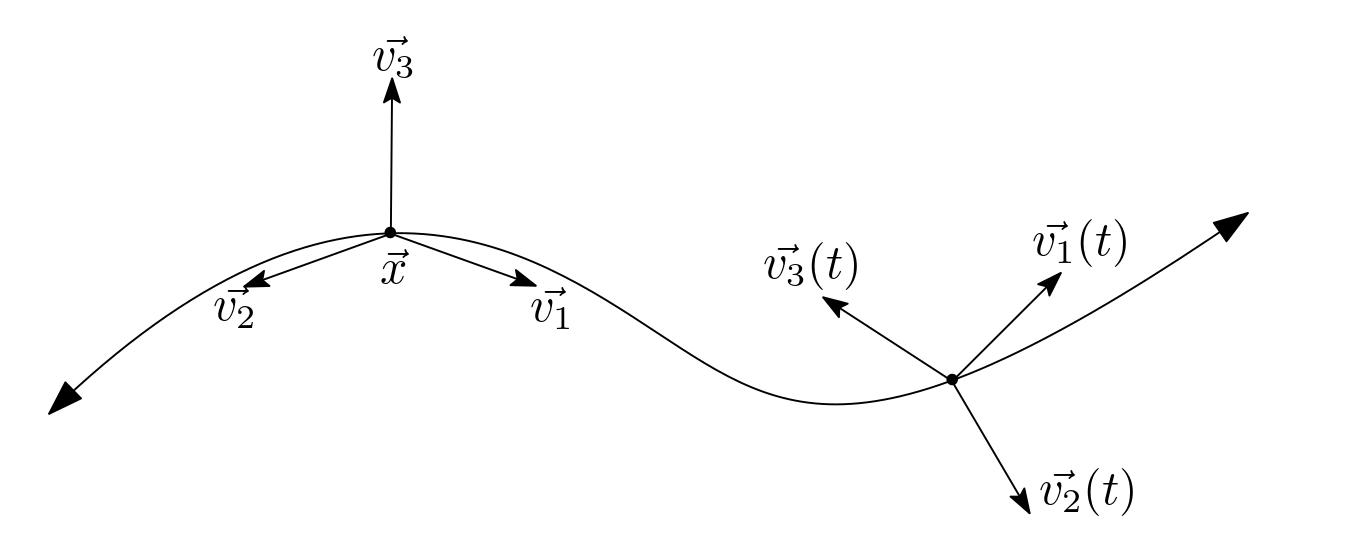
\includegraphics[width = 0.7\linewidth]{MATH314_Notes_Fig6.png}
  					\captionsetup{margin=1cm, justification=raggedright}\caption{The direction of sub-vectors change over time.}
  				\end{figure}
  				
  				\noindent The volume of the parallelepiped $\vec{v_{1}}, \vec{v_{2}}, \vec{v_{3}}$ is 
  				$$ \vec{v_{1}}\cdot (\vec{v_{2}} \cross \vec{v_{3}}) = (\epsilon, 0,0) \det 
  				\begin{vmatrix}
  					i & j& k \\
  					0 & \epsilon & 0 \\
  					\epsilon & 0 & \epsilon
  				\end{vmatrix} = \epsilon^{3}.$$
  				Note that $\vec{v_{1}}\cdot (\vec{v_{2}} \cross \vec{v_{3}}) = \vec{v_{3}} \cdot (\vec{v_{1}}\cross \vec{v_{2}})= \vec{v_{2}}\cdot (\vec{v_{3}}\cross \vec{v_{1}}).$
  				
  				\noindent We want an approximation of $\vec{v_{1}}(t) \cdot (\vec{v_{3}}(t) \cross \vec{v_{1}}(t))$, so let us compute the first order Taylor expansion of $\sigma$ centered at $\vec{x}$
  				\begin{equation*}
  					\vec{\sigma}(z,t) \approxeq \sigma(\vec{x},t) + \underbrace{D\vec{x} \sigma(\vec{x},t)}_{\text{Jacobian}} (\vec{z}-\vec{x}) \implies 
  					\vec{\sigma}(z,t) - \sigma(\vec{x},t) = D\vec{x}\sigma (x,t)(\vec{z}-\vec{x}).
  				\end{equation*}
  					At $t=0$ , we have  $\vec{z} -\vec{x} = D\vec{x}(\vec{x})(\vec{z}-\vec{x})$ ,and when $\vec{z} = \vec{x} + \epsilon\vec{i} = \vec{x} + \vec{v_{1}}$ 
  				\begin{align*}
  				&\implies \vec{v_{1}} = D\vec{x}(\vec{x}) \vec{v_{1}} = \vec{v_{1}}\\
  				\intertext{We define $\vec{v_{1}}(t) = \sigma(\vec{x} + \epsilon \vec{i} , t) - \sigma(\vec{x},t), $}
  					&\implies v_{1}(t) = D \vec{x} (\sigma(\vec{x},t))\vec{v_{1}} \\
  					&\hphantom{\implies} \:\ v_{2}(t) = D\vec{x}(\sigma(\vec{x},t))\vec{v_{2}}\\
  					&\hphantom{\implies} \:\ v_{3}(t) = D\vec{x}(\sigma(\vec{x},t))\vec{v_{3}}\\
  					&\implies \dv{}{t}v_{i}(t) = \pdv{}{t}Dx (\sigma(\vec{x},t))v_{i} = \left(Dx \pdv{}{t}\sigma(\vec{x},t)\right)\vec{v_{i}}\\
  					&\implies \underbrace{\dv{}{t}v_{i}(t)}_{\text{Vector}} = \underbrace{Dx F(\sigma(\vec{x},t))}_{\text{Matrix}}\underbrace{Dx\sigma(\vec{x},t)\vec{v_{i}}}_{\text{Matrix}}\\
  					&\implies \eval{\dv{}{t}v_{i}(t)}_{t=0} = D\vec{x} F(\vec{x})\vec{v_{i}}
  				\end{align*}
  				The volume of the parallelepiped at time $t$ is then 
  				\begin{align*}
  					v(t) &= v_{i}(t)\cdot(v_{2}(t) \cross v_{3}(t))\\
  					v'(t)&= \dv{v_{1}(t)}{t} (v_{2}(t) \cross v_{3}(t)) + v_{1}(t) \left(\dv{v_{2}(t)}{t}\cross v_{3}(t)\right) + v_{1}(t)\left(v_{2}(t) \cross \dv{v_{3}(t)}{t}\right) \\
  					&= (DxF(\vec{x})\epsilon\vec{i})(\epsilon^{2}\vec{i}) + \epsilon\vec{i}(DxF(\vec{x})\epsilon\vec{j}\cross \epsilon\vec{k}) + \epsilon\vec{i}\cdot (\epsilon\vec{j} \cross Dx F(x)\epsilon\vec{k}) \\
  					&=DxF(\vec{x})\epsilon\vec{i} \cdot \epsilon^{2}\vec{i} + DxF(\vec{x})\epsilon\vec{j} \cdot(\epsilon\vec{k}\cross \epsilon\vec{i}) + DxF(\vec{x})\epsilon\vec{k}(\epsilon\vec{i}\cross \epsilon\vec{j})\\
  					&=DxF(\vec{x})\epsilon\vec{i} \cdot \epsilon^{2}\vec{i} + DxF(\vec{x}) \epsilon\vec{j}\cdot (\epsilon^{2}\vec{j}) + DxF(\vec{x})\epsilon\vec{k}\cdot (\epsilon^{2}\vec{k})\\
  					&\hphantom{=} Dx(f(\vec{x}))\epsilon\vec{i} = 
  						\begin{bmatrix}
  							\pdv{F_{1}}{ x_{1}} & \pdv{F_{1}}{x_{2}} &\pdv{F_{1}}{x_{3}}  \\
  							\pdv{ F_{2}}{ x_{1}} & \pdv{F_{2}}{x_{2}} &\pdv{F_{2}}{x_{1}}  \\
  							\pdv{F_{3}}{x_{1}} & \pdv{F_{3}}{x_{2}} &\pdv{F_{3}}{x_{1}}  
  						\end{bmatrix}
  						\underbrace{\begin{bmatrix}
  							\vphantom{\pdv{F_{1}}{x_{1}}}\epsilon \\ \vphantom{\pdv{F_{2}}{x_{3}}}0 \\ 0\vphantom{\pdv{F_{3}}{x_{3}}}
  						\end{bmatrix}}_{\mathclap{\epsilon_{i}}}\\
  					&=\left(\epsilon \pdv{F_{1}}{x_{1}} , \epsilon \pdv{F_{2}}{x_{1}}, \epsilon \pdv{F_{3}}{x_{1}}\right) = Dx(F(\vec{x}))\epsilon\vec{i} \cdot \epsilon^{2}\vec{i} = \epsilon^{3}\pdv{F_{1}}{x_{1}} \\
  					& \hspace{2cm} \implies \eval{\dv{}{t}v(t)}_{t=0} = \epsilon^{3} \text{div} (F(\vec{x})) = V(0)\text{div}F(\vec{x})
  					\intertext{So div essentialy represents a volume changing.}
  				\end{align*}
  				\vspace{-1.5cm}
  				\begin{note}
  					The divergence of a vector field can be viewed as a \textit{volume changing}.
  				\end{note}
  				\newpage
  				
  				\section{Line Integrals and Force Fields}
  				Suppose a particle moves along a path $\sigma$ while being acted on by $\vec{F}$. We are interested in the work done on the particle as it traces out the path $\sigma$.
  				
  				\begin{figure}[H]
  					\centering
  					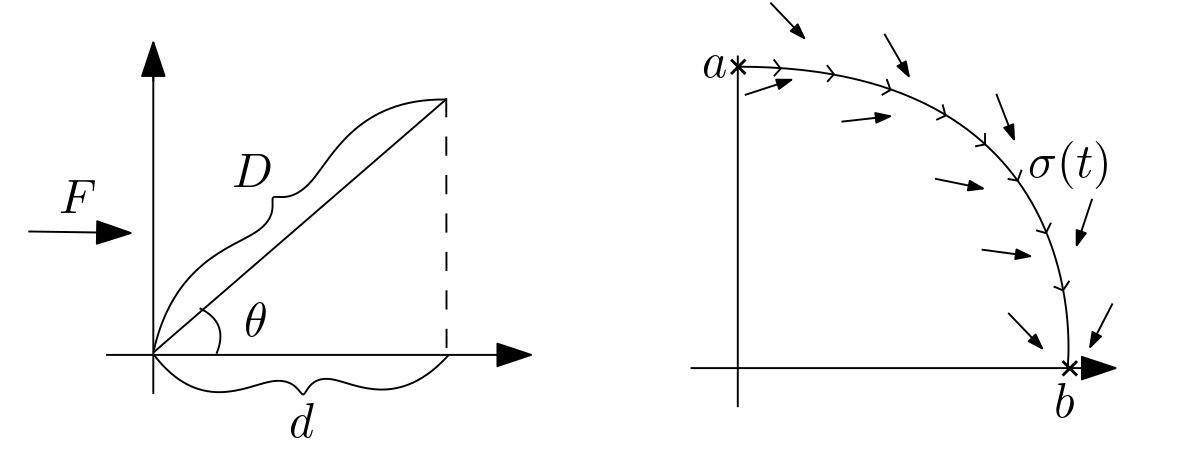
\includegraphics[width = 0.8\linewidth]{MATH314_Notes_Triple_Integral_Example4_Figure.png}
  					\captionsetup{margin=1cm, justification=raggedright}\caption{Force acting on a particle. \textbf{a)} A force $F$ is applied on a particle along a straight line.\textbf{b)} We see a force of two dimensions and the particle moves along a varying path $\sigma(t)$.}
  				\end{figure}
  				From the above figure in $a)$, the work done on the particle is along a straight line ,thus $W = FD \cos \theta = Fd.$. In the second case $b)$, Since $\sigma(t + \Delta t) - \sigma(t) \approxeq \sigma'(t) \Delta t$, the work done by the vector field at time $t$ is 
  				\begin{equation}
  					\norm{F (\sigma(t))} \norm{\sigma'(t) \Delta t} \cos \theta = F(\sigma(t))\cdot \sigma'(t)\Delta t,
  				\end{equation}
  				here we projected $F$ on the $x$-axis. 
  				\begin{equation*}
  					\text{Now, partioning} \  a= t_{0} < t_{1} < t_{2} < \dots < t_{n} < t_{n} = b \ \ , \text{the work done is} \ \ \sum_{i=0}^{n} F(\sigma(t_{i})) \cdot \sigma'(t)\Delta t.
  				\end{equation*}
  				
  				\begin{definition}[Integral along a path]
  					Let $\vec{F}$ be a vector field on $\R^{3}$ which is continuous on the $C^{1}$ path $\sigma : [a,b] \to \R^{3}$. Then we define $\int\limits_{\sigma} F\cdot ds$ , the integral of $F$ along $\sigma$ by
  					\begin{equation}
  						\int\limits_{\sigma} F\cdot ds = \int_{a}^{b} f(\sigma(t))\cdot \sigma'(t) \ dt.
  					\end{equation}
  				\end{definition}
  				
  				\begin{note}
  					Take $F = (F_{1}, F_{2} , F_{3}), \sigma = (x(t) , y(t) , z(t))$
  					\begin{equation}
	  					\implies \int\limits_{\sigma} F\cdot ds = \int_{a}^{b} F \cdot \sigma'(t) \ dt = \int_{a}^{b} \left(F_{1} \dv{x}{t} + F_{2} \dv{y}{t} + F_{3} \dv{z}{t}\right)\ dt,
  					\end{equation}
  					also frequently written as $F_{1}\ dx + F_{2} \ dy + F_{3} \ dz.$ (\textit{the differential form}).
  				\end{note}
  				
  				\begin{example}
  					Ket $\sigma(t) = (\cos^{3}(t) , \sin^{2}(t), t)  \ , t\in [0 , 7\pi/ 2]$. Compute $\int\limits_{\sigma} \sin(z) \ dx + \cos(z) \ dy - (xy)^{\sfrac{1}{3}} \ dz.$
  					\begin{align*}
  						&= \int_{0}^{\sfrac{7\pi}{2}} \sin(t) 3\cos^{2}(t)(-\sin(t)) + \cos(t)(3\sin^{2}(t))\cos(t) - \cos(t)\sin(t) \ dt\\
  						&= \frac{-1}{2} \int_{0}^{\sfrac{7\pi}{2}} \eval{\sin(2t)}_{0}^{\frac{7\pi}{2}} = \frac{-1}{2}.
  					\end{align*}
  				\end{example}
  				
  				\begin{theorem}[Fundamental Line Integral Theorem]
  					Let $\sigma : [a,b] \to \R^{3}$ be $C^{1}$ and suppose $f: \R^{3} \to \R$ is also $C^{1}$, then 
  					\begin{equation}
  						\int\limits_{\sigma} \nabla f \ ds = \int_{a}^{b} \nabla f \cdot \sigma'(t) \ dt \cdot f(\sigma (b) - f(\sigma(a)))
  					\end{equation}
  				\end{theorem}
  				
  				\begin{theorem}[Conservative]
  					If $\sigma$ is closed , $C^{1}$ curve and if $F$ is conservative, then 
  					\begin{equation} 
  					\int\limits_{\sigma} F \cdot ds = 0.
  					\end{equation}
  					Equivalently, 
  					\begin{equation} 
  					\sigma(b) = \sigma(a) \implies \int\limits_{\sigma}F\cdot ds = \int_{a}^{b} \nabla f \cdot \sigma'(t)\ dt = \int \sigma(b) - \sigma(a) = 0.
  					\end{equation}
  				\end{theorem}
  				
  				\begin{note}
	  				$F$ conservative means $F=\nabla f$.
  				\end{note}
  				
  			\subsection{Path Independence}
  				The line integral of a vector field $F$ is called path independent if for any two curves $\sigma_{1} , \sigma_{2}$, where $\sigma_{1}(a) = \sigma_{2}(a)$ and $\sigma_{1}(b) = \sigma_{2}(b)$ (i,e., they start and end at common points) , then $\int\limits_{\sigma_{1}}F\cdot ds = \int\limits_{\sigma_{2}}F\cdot ds$.
  				
  				\begin{theorem}[Path Independence]
  					\begin{equation*}
  						\int\limits_{\sigma} F\cdot ds \ \text{is path independent } \ \iff \int\limits_{c} F \cdot ds = 0 \ \forall \text{closed curve } \ c.
  					\end{equation*}
  				\end{theorem}
  				\begin{proof}
  					$(\implies)$ Assume $F$ is path independent. Take any close curve ${c : [a,b] \to \R^{3} , \ c(a) = c(b)}$. 
  					\begin{align*}
  						\raggedright
  						&\text{Let} \  a < \beta < b \\
  						&\text{Let} \ \sigma_{1} : [a,\beta] \to \R^{3} , \text{ where } \ \sigma_{1}(t) = c(t) , \ t \in [a,\beta].\\
  						&\text{Let} \ \sigma_{2} : [\beta, b] \to \R^{3} , \text{ where } \ \sigma_{2}(t) = c(t) , \ t \in [\beta, b].\\
  						&\text{Let} \ -\sigma_{2} \ \text{be the opposite direction mapping } \ c(b) \to c(\beta).
  					\end{align*}
  					Then, by path independence it follows
  					\begin{align*}
  					 \int\limits_{\sigma_{1}} F \cdot ds &= \int\limits_{-\sigma_{2}} F \cdot ds \implies \int\limits_{\sigma_{1}}F \cdot ds - \int\limits_{-\sigma_{2}}F \cdot ds = 0.
  					 \intertext{Using that $\int\limits_{\sigma}F \cdot ds = - \int\limits_{-\sigma}F \cdot ds$ , }
  					 &= \int\limits_{\sigma_{1}} F \cdot ds + \int\limits_{\sigma_{2}} F \cdot ds = 0\\
  					 &= \int\limits_{c} F \cdot ds =0.
  					 \end{align*}
  					$\hphantom{\text{  Proof.}}(\Longleftarrow)$ Suppose $\int\limits_{c} F \cdot ds = 0 $ on any closed curve. Suppose we have two paths $\sigma_{1} [a,b] \to \R^{3}$ and $\sigma_{2} [a,b] \to R^{3}$, where $\sigma_{1}(a) = \sigma_{2}(a)$ and $\sigma_{1}(b) = \sigma_{2}(b)$. Taking $\sigma_{1}$ from $a \to b$ and $-\sigma_{2}$ from $b\to a$ gives a closed curve ;
  					$$ \implies \int\limits_{\sigma_{1}}F \cdot ds + \int\limits_{-\sigma_{2}}F \cdot ds =0 \implies \int\limits_{\sigma_{1}}F \cdot ds = - \int\limits_{-\sigma_{2}}F \cdot ds = \int\limits_{\sigma_{2}}F \cdot ds, $$
  					$\therefore $ Path independent.
  				\end{proof}
  				
  				\noindent How to determine if a vector field is conservative ? Suppose $F : \R^{2} \to \R^{2}$ and $F=(P,Q)$ where $P$ and $Q$ have continuous partials. If $\nabla f = F \implies P_y = Q_x$. If $\nabla f = (P,Q) = f_x = P , \ f_y=0$, then by Clairot's theorem we have $f_{xy} = f_{yx} = P_{y} = Q_{x}$.\\
  				
  				\noindent We conclude that if $F$ is conservative with $F= (P,Q)$ where $P,Q$ have continuous partials then $P_{y} = Q_{x}$. Now a question arises, if $F=(P,Q)$ and $P_{y} = Q_{x}$ does there exist a function $f$ such that $f_{x} = P $ and $f_{y} = Q$ ? This is only true for certain domains, which leads us to the next important definitions.
  				
  				\begin{definition}[Simple Closed Curve]
  					A simple closed curve is a curve $\sigma : [a,b] \to \R^{n}$ which does not intersect itself outside of its endpoints which implies that $\sigma(t_{i})= \sigma(t_{j})$ for $a \le t_{i} \le t_{j} \le b \implies t_{i} = a ,  \ t_{j} = b$.
  				
  				%TODO  schematics of simple coneected and not simple connected
  				\end{definition}
  				
  				\begin{definition}[(Path) Connected]
  					A domain $D$ is called (path) connected if any two points in $D$ can be joined by a path that lies in $D$.
  				\end{definition}
  				
  				\begin{definition}[Simply Connected ]
  					A simply connected region $D$ is a connected region such that every simple closed curve in $D$ encloses points only contained in $D$. 
  				\end{definition}
  				\vspace{-0.5cm}
  				\begin{figure}[H]
  					\centering
  					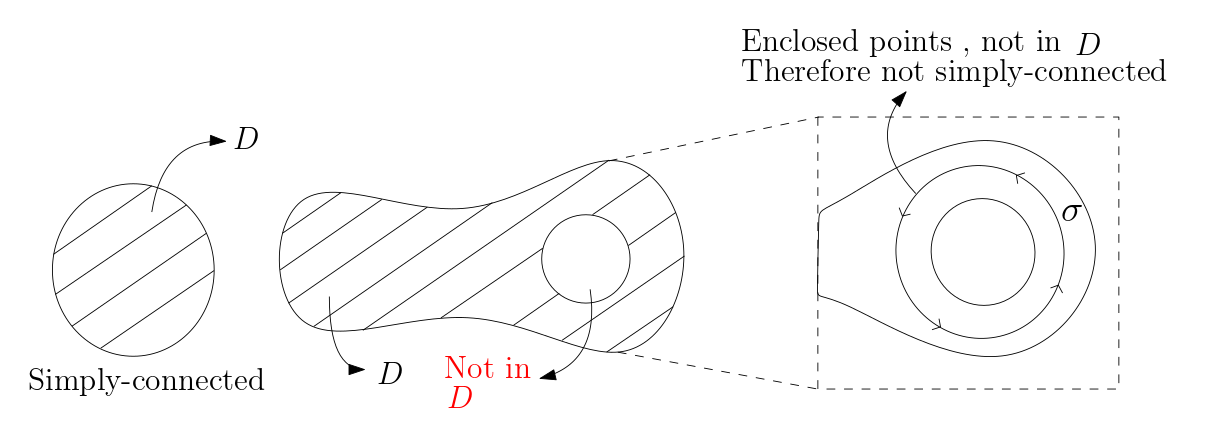
\includegraphics[width=\linewidth]{MATH314_Notes_Triple_Integral_Example5_Figure.png}
  					\captionsetup{margin=1cm, justification=raggedright}\caption{Illustration of simply-connected and not simply-connected domains, following the previous definitions.}
  				\end{figure}
  				
  				\begin{theorem}
  					If $F = (P,Q)$ is a vector field on a open simply connected region $D$ and $P,Q$ have continuous partials with $\pdv{P}{y} = \pdv{Q}{x}$ then $F$ is conservative $(F = \nabla f \ \text{where } \ f \in C^{1}).$
  				\end{theorem}
  				
  				\begin{theorem}
  					Let $F = (F_{1}, F_{2}, F_{3})$ with partials of $F_{i}$ continuous in $D$. If curl$\vec{F} = \vec{0}$ in $D$ and $D$ is simply connected, then $F$ is conservative $(F = \nabla f, f \ \text{is }\ C^{1}).$
  				\end{theorem}
  				
  				\begin{example}
  					Let $F+ (3 + 2xy , x^{2}-3y^{2})$ , determine if $F$ is conservative. If so, find $f$ such that $\nabla f = F$.
  					\begin{itemize}
  						\item \textbf{Step 1:} Check $\pdv{}{y} (3+2xy) = \pdv{}{x}(x^{2}-3y^{2}).$ 
  						\item \textbf{Step 2:} Is the domain simply connected ?  
  					\end{itemize}
  					$\pdv{}{y}(3+2xy) = 2x , \ \pdv{}{x}(x^{2} - 3y^{2})=3x \ \ \therefore \ \text{same}.$ Moreover, $F$ has polynominal components therefore no singularities. Which then implies that the domain is simply connected and consequently $F$ is conservative.
  					
  					\noindent Now how do we find $f$ such that $\nabla f = F$? Conservative implies that $F = (f_{x} , f_{y}).$ We use the procedure for Exact Equations from ODEs ; 
  					\begin{gather*}
  						\implies \pdv{}{x} f(x,y) = 3+2xy \implies f(x,y) = \int  3+2xy dx + g(y) \implies f(x,y) = 3x + x^{2}y + g(y).
  						\intertext{We use $f_{y} = x^{2} - 3y^{2}$ and get ,}
  						\pdv{}{y} f(x,y) = x^{2} + g^{\prime}(y) = x-2y^{2} \implies g'(y) = -3y^{2} \implies g(y) = -y^{3}.\\
  						\therefore f(x,y) = 3x + x^{2}y -y^{3}.
   					\end{gather*} 
  				\end{example}
  				
  				\begin{example}
  					Show that $\int\limits_{C} 2xe^{-y} \ dx + (2y -x^{2}e^{-y})dy$ is path independent. 
  					
  					\noindent First we show that $F=(2xe^{-y} , 2y-x^{2}e^{-y})$ is conservative 
  					$$ \pdv{}{y}(2xe^{-y}) = -2xe^{-y}\quad , \pdv{}{x} (2y-x^{2}e^{-y})=-2xe^{-y} \ \ \checkmark. $$
  					And, since both components are sums of products of polynomials and exponential this implies there are no singularities and consequently $F$ is conservative. 
  				\end{example}
  				
  			\subsection{Green's Theorem}
  				We say a simple closed curve has positive orientation if the closed curve is traced on counter-clockwise.
  				
  				\begin{figure}[H]
  					\centering 
  					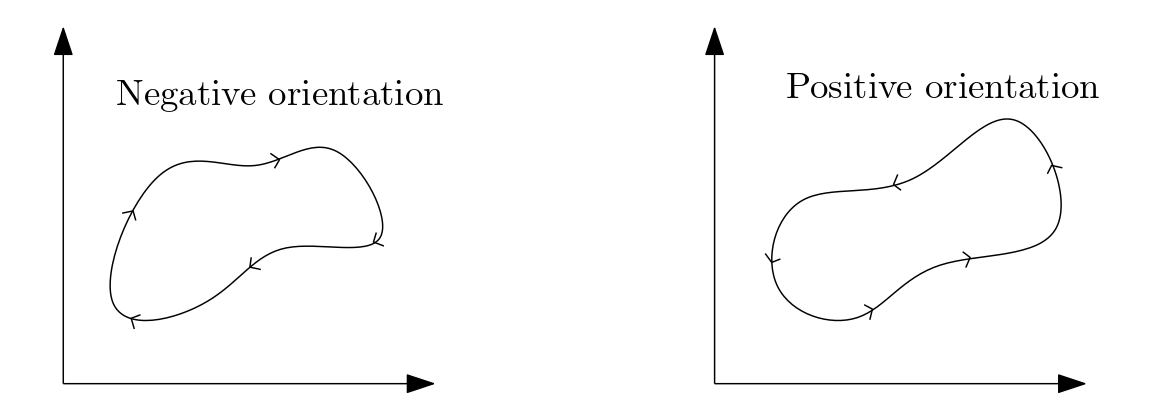
\includegraphics[width=0.9\linewidth]{MATH314_Notes_Triple_Integral_Example6_Figure.png}
  					\captionsetup{margin=1cm, justification=raggedright}\caption{Positive and negative orientation of a closed curve.}
  				\end{figure}
  				
  				\begin{theorem}[Green's Theorem]
  					Let $C$ be a positively oriented piece wise smooth , simple closed curve in the plane and let $D$ be the region bounded by $C$. If $P(x,y)$ and $Q(x,y)$ have continuous partials on an open region containing $D$, then 
  					\begin{equation} 
  					\int\limits_{C} Pdx + Qdy = \iint\limits_{D}\dv{Q}{x} - \dv{P}{y} \ dA.
  					\end{equation}
  				\end{theorem}
  				\begin{proof}
  					\begin{figure}[H]
  						\centering
  						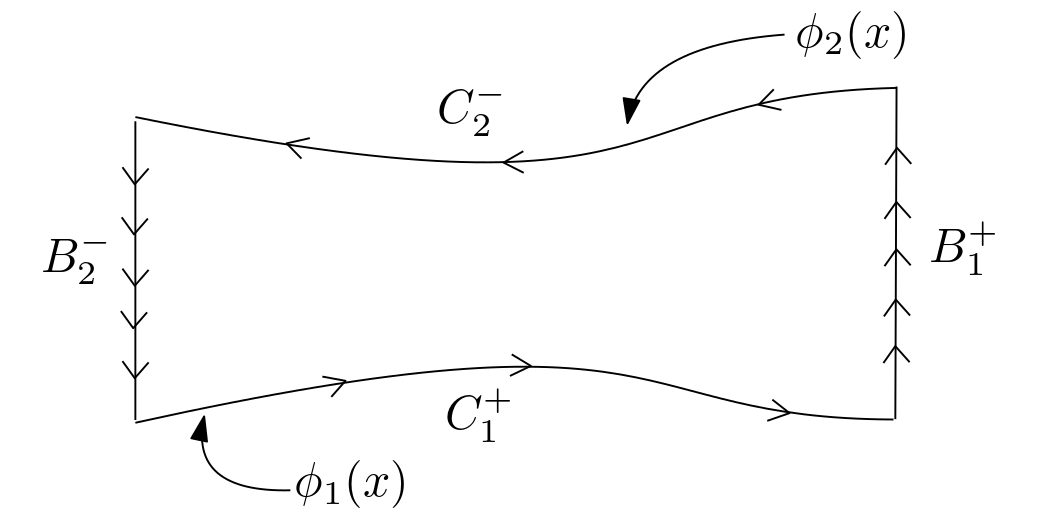
\includegraphics[width=0.5\linewidth]{MATH314_Notes_Triple_Integral_Example7_Figure.png}
  						\captionsetup{margin=1cm, justification=raggedright}\captionsetup{margin=2cm, justification=raggedright}
  						\captionsetup{margin=1cm, justification=raggedright}\caption{A type $1$ domain $D$ for, figure for illustrative purpose and to facilitate the proof's notation.}
  					\end{figure}
  					We start the proof by assuming $D$ is of type $1$ ,
  					\begin{gather*}
  						D:= x\in [a,b] , \ \varphi_{1}(x) \le y \le \varphi_{2}(x) \qquad ,
  						C^{+} = C_{1}^{+} \cup B_{1}^{+} \cup C_{2}^{-} \cup B_{2}^{-} ,\\
  						\text{Show that }  \ \int\limits_{C^{+}} Pdx = \iint\limits_{D} \pdv{P}{y} dA. \\ 
  						\iint\limits_{D} \pdv{P}{y} dA = \int_{a}^{b} \int_{\varphi_{1}(x)}^{\varphi_{2}(x)} \pdv{P}{y} \ dy dx = \int_{a}^{b} P(x, \varphi_{2}(x)) - P(x, \varphi_{1}(x)) \ dx
  						\intertext{Notice that  } 
  						 \int_{a}^{b} P(x, \varphi_{2}(x)) dx = \int\limits_{-C_{2}^{-}}P \ dx = - \int\limits_{C_{2}^{-}} P \ dx.
  						\intertext{Also notice that similarly }
  						-\int_{a}^{b} P(x, \varphi_{1}(x)) \ dx = - \int\limits_{C_{1}^{+}} P  \ dx.
  						\intertext{Since $x$ is constant on $B_{1}^{+}$ and $B_{2}^{+}$ , $\implies$ $\int\limits_{B_{1}^{+}}Pdx = 0 = \int\limits_{B_{2}^{-}} Pdx$.}
  						\intertext{Putting this all tohether we get, }
  						\iint\limits_D \pdv{P}{y} dA = - \int\limits_{C_{1}^{+}}Pdx - \int\limits_{C_{2}^{-}}Pdx - \int\limits_{B_{1}^{+}}Pdx - \int\limits_{B_{2}^{-}}Pdx = - \int\limits_{C^{+}}Pdx.
  					\end{gather*}
  				\end{proof}
  				
  				\begin{theorem}
	  				If $\sigma$ is a simple closed curve which bounds domain $D$ , where $\sigma = \partial D$ (boundary of $D$), then 
	  				\begin{equation} 
	  				\text{Area of $D$ is } \ \frac12 \int\limits_{\partial D} xdy -y dx.
	  				\end{equation}
  				\end{theorem}
  				
  				\begin{proof}
  					Area($D$)$= \frac12 \int\limits_{\partial D} -ydx + xdy.$ By the Green's theorem this imply that $P(x,y) = -y$ and $Q(x,y) = x$.
  					$$ \implies \frac12 \int\limits_{\partial D}-ydx + xdy = \frac12 \iint\limits_{D} \pdv{Q}{x} - \pdv{P}{y} \ dA = \iint\limits_{D} \ dA \ \ \checkmark.$$
  				\end{proof}
  				
  				\noindent Now what if the region is not of type $3$ ? The idea is to take the region, divide it in two sub regions and apply our machinery to those sub-regions. 
  				
  				\begin{figure}[H]
  					\centering
  					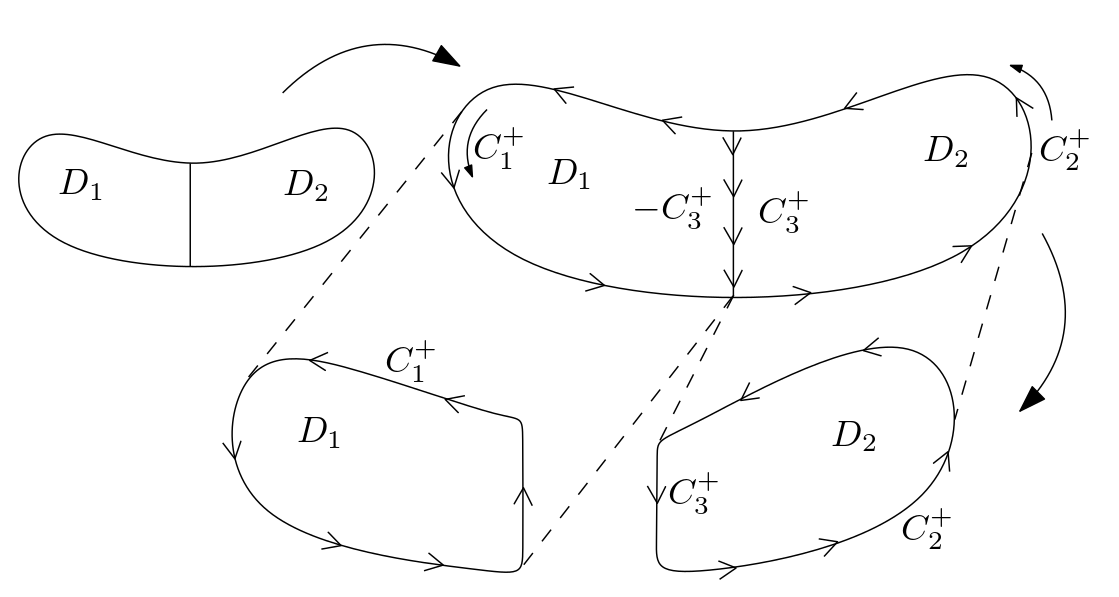
\includegraphics[width=0.8\linewidth]{MATH314_Notes_Triple_Integral_Example8_Figure.png}
  					\captionsetup{margin=1cm}
  					\caption{How to handle regions that are not type $3$.}
  				\end{figure}
  				
  				\noindent Following Figure $19$ , let us show rigorously that Green's theorem holds for these types of regions. 
  				$$ \iint\limits_{D_{1}}\pdv{Q}{c} - \pdv{P}{y} \ dA = \int\limits_{C_{1}^{+}\cup -C_{3}^{+}} Pdx - Qdy \quad , \iint\limits_{D_{2}}\pdv{Q}{c} - \pdv{P}{y} \ dA = \int\limits_{C_{2}^{+}\cup C_{3}^{+}} Pdx - Qdy .$$
  				\begin{align*}
  					\iint\limits_D \pdv{Q}{x} - \pdv{P}{y} \ dA &= \iint\limits_{D_{1}}\pdv{Q}{c} - \pdv{P}{y} \ dA +  \iint\limits_{D_{2}}\pdv{Q}{c} - \pdv{P}{y} \ dA  \\
  					&= \int\limits_{C_{1}^{+}} Pdx + Qdy -\int\limits_{C_{3}^{+}} Pdx + Qdy + \int\limits_{C_{2}^{+}} Pdx + Qdy  \int\limits_{C_{3}^{+}} Pdx + Qdy  \\
  					&= \iint \pdv{Q}{x} - \pdv{P}{y} \ dA = \int\limits_{C_{1}^{+}\cup C_{2}^{+}} Pdx + Qdy = \int\limits_{C^{+}}Pdx +qdy.
  				\end{align*}
  				$\therefore \ $ Green's theorem holds on the union of type $3$ regions.
  				
  				\begin{example}
  					Verify Green's theorem in the unit disc where $P(x,y) =x$ ,  $Q(x,y) = xy$.
  					
  					\noindent Recall Green's theorem states that 
  					$$ \int\limits_{C} Pdx +Qdy = \iint\limits_{D} \pdv{Q}{x} - \pdv{P}{y} \ dA.$$
  					
  					\noindent Note that this corresponds to a circle of path $\sigma(t) = (\cos(t),\sin(t)) \equiv (x(t),y(t))$, with domain $D$ inside. Let us first verify the left hand side of the above formula then the RHS.
  					\begin{align*}
  						\int\limits_{\sigma}Pdx + Qdy &= \int_{0}^{2\pi}P(x(t), y(t))x'(t) + Q(x(t) ,y(t))y'(t)\\
  						&= \int_{0}^{2\pi}\cos(t)(-\sin(t))+ \cos^{2}(t)\sin(t) \ dt\\
  						&\stackrel{u = \cos(t)}{=} \int_{1}^{1}u-u^{2} \ du =0.
  					\end{align*}
  					Now for the RHS,
  					$$ \iint\limits_{D} \pdv{Q}{x} - \pdv{P}{y} \ dA = \iint\limits_{D} y \ dA = \int_{0}^{2\pi}\int_{0}^{1} r^{2}\sin \theta \ drd\theta =\int_{0}^{2\pi}\frac{\sin\theta}{3}\ d\theta = 0.$$
  					Green's theorem is verified. 
  				\end{example}
  				
  				\noindent On the previous class we proved Green's theorem on type $3$ domains i.e.,
  				\begin{equation*}
  					\begin{rcases}
  						D:= &x\in [a,b] , \varphi_{1}(x) \le y \le \varphi_{2}(x) \\
  						\text{or} \ &y\in [c,d]  , \varphi_{1}(y) \le x \le \varphi_{2}(y)
  					\end{rcases} \ \ \text{Equivalent ways to write.}
  				\end{equation*}
  				
  				What if the domain is not of type $3$ ? 
  				\begin{figure}[H]
  					\centering
  					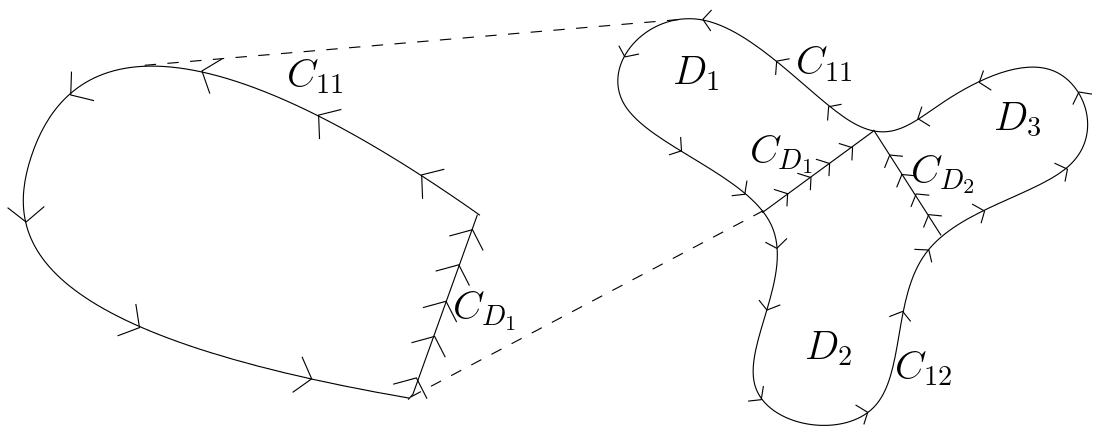
\includegraphics[width=0.8\linewidth]{MATH314_Notes_Triple_Integral_Example9_Figure.png}
  					\caption{Other example of non type $3$ domain.}
  					\captionsetup{margin = 1cm}
  				\end{figure}
  				
  				\noindent Following Figure $20$, let us suppose $D_{1}, D_{2}, D_{3}$ are type $3$. Then we want to do,
  				\begin{align*}
  					&\iint\limits_{D}\pdv{Q}{x} - \pdv{P}{y} \ dA = \iint\limits_{D_{1}} \pdv{Q}{x} - \pdv{P}{y} \ dA + \iint\limits_{D_{2}}\pdv{Q}{x} - \pdv{P}{y} \ dA + \iint\limits_{D_{3}} \pdv{Q}{x} - \pdv{P}{y} \ dA \\
  					\text{so , } &\iint\limits_{D_{1}}\pdv{Q}{x} - \pdv{P}{y} \ dA = \int\limits_{C_{11}} Pdx + Qdy + \int\limits_{C_{D_{1}}}Pdx + Qdy \\
  					&\iint\limits_{D_{2}}\pdv{Q}{x} - \pdv{P}{y} \ dA =\underbrace{ \int\limits_{C_{12}}Pdx + Qdy + \int\limits_{C_{D_{2}}}Pdx + Qdy \overbrace{-\int\limits_{C_{D_{1}}}Pdx + Qdy}^{\int\limits_{-C_{D_{1}}} = - \int\limits_{C_{D_{1}}}}}_{\text{all these components to complete one loop}} \\
  					&\iint\limits_{D_{3}}\pdv{Q}{x} - \pdv{P}{y} \ dA = \int\limits_{C_{13}}Pdx + Qdy - \int\limits_{C_{D_{2}}}Pdx + Qdy.
  					\intertext{Recollecting , many terms cancel out so then we have}
  					&\quad \iint\limits_{D} \pdv{Q}{x} - \pdv{P}{y} \ dA = \int\limits_{C_{11}}Pdx + Qdy +\int\limits_{C_{12}}Pdx + Qdy  +\int\limits_{C_{13}}Pdx + Qdy .
  				\end{align*}
  				Letting $c:=C_{11} \cup C_{12} \cup C_{12} = \partial D$ we get 
  				$$ \iint\limits_{D} \pdv{Q}{x} - \pdv{P}{y} \ dA = \int\limits_{C = \partial D} Pdx + Qdy.$$\\
  				
  				\noindent Now what about regions enclosed by $2$ closed curves ? 
  				\begin{figure}[H]
  					\centering
  					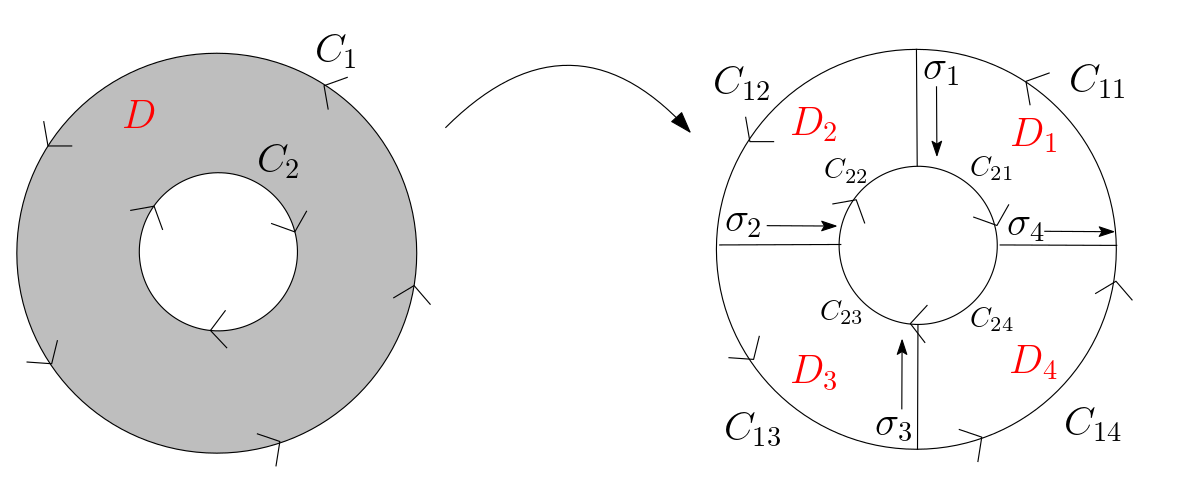
\includegraphics[width = 0.8\linewidth]{MATH314_Notes_Triple_Integral_Example19_Figure.png}
  					\captionsetup{margin=1cm}
  					\caption{Example of transforming non-type $3$ domain enclosed by two curves ,into a type $3$ domain.}
  				\end{figure}
  				
  				\noindent Following Figure $21$, note that in the LHS picture , $C_{1}$ is positively oriented while $C_{2}$ is negatively oriented , as stated in Figure $17$. We can immediately apply Green's theorem, first of , let $C_{1} = C_{11} \cup C_{12} \cup C_{13} \cup C_{14}$ and let $C_{2} = C_{21} \cup C_{22} \cup C_{23} \cup C_{24}$. We then have, by definition 
  				\begin{equation*}
  				\begin{multlined}[t]
  				 \iint\limits_{D} \pdv{Q}{x} - \pdv{P}{y} \ dA =\iint\limits_{D_{1}} \pdv{Q}{x} - \pdv{P}{y} \ dA + \iint\limits_{D_{2}} \pdv{Q}{x} - \pdv{P}{y} \ dA \hspace{-0.2cm}\\+ \iint\limits_{D_{3}} \pdv{Q}{x} - \pdv{P}{y} \ dA + \iint\limits_{D_{4}} \pdv{Q}{x} - \pdv{P}{y} \ dA.
  				 \end{multlined}
  				 \end{equation*}
  				Using Figure $20$, we can express each integral on the RHS as follows ,
  				\begin{alignat*}{2}
  					&\iint\limits_{D_{1}} \pdv{Q}{x} - \pdv{P}{y} \ dA = \int\limits_{\mathclap{C_{11}\cup \sigma_{1}\cup C_{21} \cup \sigma_{1}}} Pdx + Qdy \qquad , && \iint\limits_{D_{2}} \pdv{Q}{x} - \pdv{P}{y} \ dA = \int\limits_{\mathclap{C_{12}\cup \sigma_{2} \cup C_{22}\cup -\sigma_{1}}}Pdx + Qdy \\
  					&\iint\limits_{D_{3}} \pdv{Q}{x} - \pdv{P}{y} \ dA = \int\limits_{\mathclap{C_{13}\cup \sigma_{3}\cup C_{23} \cup -\sigma_{2}}} Pdx + Qdy \qquad , && \iint\limits_{D_{4}} \pdv{Q}{x} - \pdv{P}{y} \ dA = \int\limits_{\mathclap{C_{14}\cup -\sigma_{4} \cup C_{24}\cup -\sigma_{3}}}Pdx + Qdy. 
  				\end{alignat*}
  				Adding this all up, all the $\sigma_{i}$ cancel and we are left with 
  				$$ \iint\limits_{D}\pdv{Q}{x} - \pdv{P}{y} \  dA = \int\limits_{C_{1}}Pdx + Qdy + \int\limits_{C_{2}}Pdx + Qdy.$$
  				
  				\begin{example}
  					Let $F(x,y) = \left(\frac{-y}{x^{2}+y^{2}} , \frac{x}{x^{2}+y^{2}}\right)$, show that $\int\limits_{\sigma} F\cdot ds = 2\pi$ , for any simple closed curve $\sigma$ enclosing (wraps around it) the point $(0,0)$. Assume $\sigma$ is positively oriented.\\
  					
  					\noindent The strategy for this type of problem is as follows , first , find a circle of radius $a$ centered at $(0,0)$ which is contained in the region enclosed by $\sigma$. Then solve for $c(t) = (a\cos(t) , a\sin(t))$ , for some $a > 0$. Replacing in Figure $21$a $ \ $ $C_{1}$ by $\sigma$ and $C_{2}$ by $C$ whilst allowing a non-circular shape and allowing a negative orientation for $C$, we have our corresponding domain. Given $F$ as defined and since the region enclosed by $C$ is not in the domain we can say that $F$ has continuous partials on $D$, therefore, 
  					$$ \iint\limits_{D} \pdv{Q}{x} - \pdv{P}{y} \ dA = \int\limits_{\sigma} Pdx + Qdy - \int\limits_{C} Pdx + Qdy, $$
  					here we're subtracting since $C$ and $\sigma$ have opposite directions. Note that we chose the directions of $C$ and $\sigma$ purely arbitrarily , as longs as we stay consistent with the signs in the previous equation everything should remain consistent as well.
  					
  					Now let's go back to our function $F$, 
  					\begin{gather*}
  						F(x,y) = \left(\frac{-y}{x^{2}+y^{2}} , \frac{x}{x^{2}+y^{2}}\right)\implies P = \frac{-y}{x^{2}+y^{2}} , \: Q = \frac{x}{x^{2} + y^{2}} \\
  						\text{Therefore ,} \pdv{Q}{x} = \frac{x^{2} + y^{2} -2x^{2}}{(x^{2}+y^{2})^{2}} = \frac{y^{2}-x^{2}}{(x^{2} + y^{2})^{2}}. \\
  						\text{And similarly, } \pdv{P}{y} = \frac{-(x^{2}+y^{2})+2y^{2}}{(x^{2}+y^{2})^{2}} = \frac{y^{2}-x^{2}}{(x^{2}+y^{2})^{2}} \\
  						\therefore \ \text{by Green's theorem, } \iint\limits_{D} \pdv{Q}{x} - \pdv{P}{y} \ dA = \iint\limits_{D}\left(\frac{y^{2}-x^{2}}{(x^{2}+y^{2})^{2}}\right) -\left(\frac{y^{2}-x^{2}}{(x^{2}+y^{2})^{2}}\right) \ dA = 0.
  					\end{gather*}
  					This result then implies that 
  					$$ \int\limits_{D} F \cdot ds = \int\limits_{C} F \cdot ds.$$
  					We may now compute the path integral, 
  					\begin{align*}
  						\int\limits_{\sigma} F \cdot ds &= \int_{0}^{2\pi} F(a\cos(t) , a\sin(t))\cdot \underbrace{(-a\sin(t), a\cos(t))}_{\mathclap{\text{$\sigma'(t)$ from the path integral definition}}} \ dt \\
  						&= \int_{0}^{2\pi} \frac{-a\sin(t)}{a^{2}\cos^{2}(t) + a^{2}\sin^{2}(t)}(-a\sin(t)) + \frac{a\cos(t)}{a^{2}\cos^{2}(t) + a^{2}\sin^{2}(t)}(a\cos(t)) \ dt \\&= \int_{0}^{2\pi} \ dt = 2\pi.
  					\end{align*}
  				\end{example}
  				
  				\begin{theorem}
  					Let $F =(P,Q)$ be a vector field on a simply connected domain $D$ where $P$ and $Q$ have continuous partials on $D$ and $\pdv{P}{y} = \pdv{Q}{x}$ on $D$. Then, $\int\limits_{C} F \cdot ds =0$ for any simple closed curve $c$ contained in $D$.
  				\end{theorem}
  				\begin{proof}
  					Follows from Green's theorem !
  				\end{proof}
  				
  			\subsection{Vector Form of Green's Theorem}
  				Let $D$ be a simply connected region of $\R^{2}$ which can be portioned into type $3$ domains. Let $\partial D  = C$, positively oriented. Letting $F$ be  $C^{1}$ vector field on $D$ , we have
  				\begin{equation}
  					\int\limits_{\partial D} F \cdot ds = \int\limits_{C} F \cdot ds = \iint\limits_{D}(\text{Curl}F)\cdot \vec{k} \ dA = \iint\limits_{D} (\nabla \cross F)\cdot \vec{k} \ dA,
  				\end{equation}
  				where $\vec{k}$ is the usual unit vector $(0,0,1)$.\\
  				
  				\noindent Taking $F = (P,Q,0)$  and recalling \eqref{eq_curl_matrix}
  				\begin{gather*}
  					\implies \text{Curl }F = \det 
  					\begin{vmatrix}
  						\vec{i} & \vec{j}& \vec{k} \\
  						\pdv{}{x} & \pdv{}{y} & \pdv{}{z} \\
  						P & Q & 0
  					\end{vmatrix} = \left(0,0,\pdv{Q}{x} - \pdv{P}{y}\right)\\
  					\therefore (\text{Curl}F)\cdot \vec{k} = \pdv{Q}{x}- \pdv{P}{y} \ \ \text{Standard form of Green's theorem}
  				\end{gather*}
  				
  				\begin{theorem}[Difergence Theorem in $\R^{2}$]
  					Let $D\subseteq \R^{2}$ be simply connected and a union of type $3$ domain. Let $\sigma(t) : [a,b] \to \R^{2}$ be a positively oriented parametrization of the boundary $\partial D$, where $\sigma(t) = (x(t), y(t))$. 
  					
  					Let $\vec{n}$ denote the unit outward normal of $\partial D$, given by 
  					\begin{equation} 
  					\vec{n} = \frac{(y'(t) - x'(t))}{\sqrt{(x'(t))^{2} + (y'(t))^{2}}}.
  					\end{equation}
  					Then, if $F$ is $C^{1}$ vector field on $D$ we have,
  					\begin{equation} 
  					\int\limits_{\partial D = \sigma}F \cdot \vec{n} \ ds = \iint\limits_{D} \textrm{Div}{F} \ dA.
  					\end{equation}
  				\end{theorem}
  				
  				\begin{remark}
  					$\vec{n}$ is a vector perpendicular to $\sigma'(t)$ which implies that $\vec{n} \cdot \sigma'(t) = 0.$
  				\end{remark}
  				
  				\begin{note}
  					$\vec{F} \cdot \vec{n}$ is a scalar, i.e., a real-valued function. Therefore, $\int\limits_{\sigma}F\cdot \vec{n}$ is a path integral.
  				\end{note}
  				
  				Let $F(x,y) = (P(x,y) , Q(x,y))$ then 
  				\begin{align*}
  					\int\limits_{\sigma} \vec{F} \cdot \vec{n} \ ds &= \int_{a}^{b}\left(\frac{P(x(t), y(t))y'(t)}{\sqrt{(x'(t))^{2} + (y'(t))^{2}}} - \frac{Q(x(t) , y(t))x'(t)}{\sqrt{(x'(t))^{2} + (y'(t))^{2}}}\right) \sqrt{(x'(t))^{2} + (y'(t))^{2}} \ dt\\
  					&= \int\limits_{\sigma}Pdy - Qdx 
  					\intertext{Observe the previous equation, usual Green's theorem is $\int\limits_{\sigma}P\textbf{$dx$} + P\textbf{$dy$}$.} 
  					&= \int\limits_{\sigma}(-Q)dx + Pdy = \iint\limits_{D} \pdv{P}{x} + \pdv{Q}{y} \ dA = \iint\limits_{D} \textrm{Div}{F} \ dA.
  				\end{align*} 
  				
  				\rule{\linewidth}{0.4 pt}
  				
  				What will we cover in the next two remanding weeks ? Green's theorem is finished and line integrals , path integrals , curl, div ... Now we need to do \textit{surface integrals} (integrals over surface in 3D). \textit{Stoke's theorem (generalization of Green's in 3D)} and \textit{divergence theorem}. 
  				
  				\section{Parametric Surfaces}
				So far we have looked at surfaces given by the graph of a function $z = f(x,y) $, where $f(x,y) : \R^{2} \to \R,$ but also level surfaces like $k = f(x,y,z)$. 
				
				\begin{definition}[Parametric surface]
					A parameterized surface also known as a parametric surface is a function $\phi : D \subset \R^{2} \to \R^{3}.$ This surface, denoted $S$ corresponding to the function $\phi$ is its image $S = \phi (D)$.
					
					We can write $\phi (u,v) = (x(u,v), y(u,v) , z(u,v)).$ We say $S$ is a differentiable surface if $\phi$ is differentiable $\implies$ $x(u,v), y(u,v) $ and $z(u,v)$ are differentiable.
				\end{definition} 				
					Think of these as an extension of parametric curves $\vec{r}(t) = (x(t) , y(t), z(t))$ , to surfaces. 
					So if we're going to vary $u$ and $v$ everywhere in the domain this is going to create a surface in $\R^{3}$.
					
				\begin{example}
					Identify the parametric surface
					$$ x = u\cos (v) , y= u \sin (v) , z = u \quad u\ge 0.$$
					Note there's both a $\cos$ and a $\sin$ with $u$ in front. 
					\begin{align*}
						&\implies x^{2} + y^{2} = u^{2}(\cos^{2}(v) + \sin^{2}(v)) \\
						&\hphantom{\implies x^{2} + y^{2}}= u^{2} \\
						&\implies z = \sqrt{x^{2} + y^{2}}
					\end{align*}
					Therefore this is a cone. Hence, $(u\cos(v) , u\sin(v), u)$ parameterizes a cone. 
				\end{example}
				
				\begin{definition}[Smoothness (\textit{Informal})]
					We say a surface is smooth is there exists a tangent plane at any point of that surface.
				\end{definition}
				\begin{figure}[H]
				\centering
					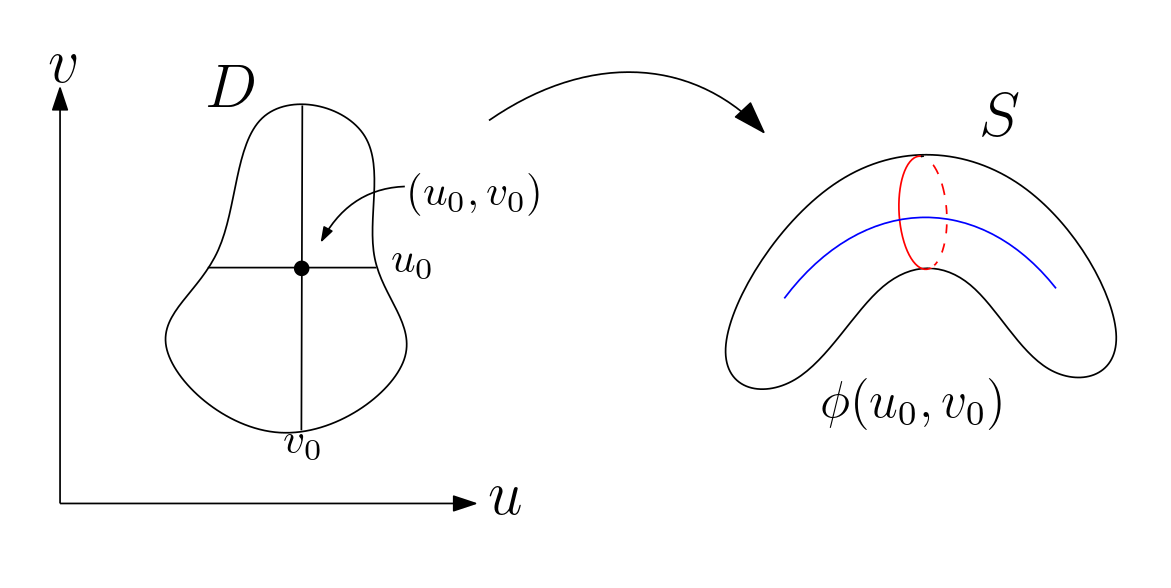
\includegraphics[width= 0.8\linewidth]{MATH314_Notes_Fig7.png}
					\captionsetup{margin=1cm, justification=raggedright} \caption{\textbf{a)} Two dimensional surface living in $\R^{2}$. \textbf{b)} The surface $S$ living in $\R^{3}$ ; \color{blue} Line projected while $v_{0}$ is fixed, \color{red} Line projected while $u_{0}$ is fixed. \color{black}}
				\end{figure}
				
				\noindent Following Figure 22, suppose we fix $u=u_{0}$ and let $v$ vary in $D$. This implies $\varphi(u_{0},v) = (x(u_{0},v) , y(u_{0} , v) ,z(u_0 , v))$ is a parametric curbe on $S$. The vector tangent to the curve $\varphi(u_{0} , v)$ at $\varphi(u_{0} , v_{0})$ is 
				\begin{align*} 
				\vec{T}_{v} := \pdv{x}{v}(u_{0}, v_{0}) ,\pdv{y}{v} (u_{0} ,v_{0}) , \pdv{z}{v}(u_{0},v_{0}) := \pdv{x}{v}(u_{0}, v_{0})\vec{i} + \pdv{y}{v} (u_{0} ,v_{0})\vec{j} + \pdv{z}{v}(u_{0},v_{0})\vec{k}.
				\end{align*}
				Similarly, fixing $v_{0}$ and letting $u$ vary in $D$ , we obtain the tangent vector at $\varphi(u_{0},v_{0})$
				$$ \vec{T}_{u} := \pdv{x}{u}(u_{0}, v_{0})\vec{i} + \pdv{y}{u} (u_{0} ,v_{0})\vec{j} + \pdv{z}{u}(u_{0},v_{0})\vec{k}.$$
				Using $\vec{T}_{u}$ and $\vec{T}_{v}$ we can form the tangent plane to $S$ at $\varphi(u_{0} , v_{0})$ by computing the normal vector 
				$$ \vec{n} = \vec{T}_{u} \cross \vec{T}_{v}.$$
				Putting this all together we have the following definition 
				\begin{definition}[Smoothness (\textit{Formal})]
					A parameterized surface is smooth at a point $(u_{0},v_{0})$ if $\vec{T}_{u}\cross \vec{T}_{v} \neq \vec{0}$ at $(u_{0},v_{0})$. \\
					
					\noindent Moreover, we say $S$ is smooth if $\vec{T}_{u}\cross \vec{T}_{v} \neq \vec{0}$ anywhere in $D$ (or all points $\varphi(u,v) \in S$).
				\end{definition}
				
				\noindent Having defined smoothness let us analyse the previous example (\textbf{Example 10.1}).
				\begin{example*}
					We had,
						$$ x = u\cos (v) , y= u \sin (v) , z = u \quad u\ge 0.$$
					\begin{itemize}
						\item Is the surface differentiable ? The surface is indeed differentiable because $x,y,z$ are all differentiable functions. Recalling Section 3, product of polynomial functions is differentiable given the components are differentiable.
						\item Is the surface smooth ? 
					\end{itemize}
					\begin{gather*}
						\vec{T}_{u} = (\cos(v),\sin(v),1) ,\qquad \vec{T}_{v} = (-u\sin(v), u\cos(v), 0)\\
					\end{gather*}
					\vspace{-1.5cm}
					\begin{align*}
						\vec{T}_{u} \cross \vec{T}_{v} &= \det 
						\begin{vmatrix}
							\vec{i} & \vec{j} & \vec{k} \\
							\cos(v) & \cos(v) & 1 \\
							-u\sin(v) & u\cos(v) & 0
						\end{vmatrix} \\
						&= (-u \cos(v) ,-u\sin(v), u\cos^{2}(v) + u\sin^{2}(v)).
					\end{align*}
					Notice that when $u=0$ , we have $\vec{T}_{u} \cross \vec{T}_{v} = \vec{0}$, $\therefore$ the surface is not smooth. Indeed, the point at the sharp end of a cone has no tangent plane there !
				\end{example*}
				\begin{example}
					Find the tangent plane to the surface 
					$$ x = u^{2} , y=v^{2} , z= u+2v \qquad \text{ at } \ (1,1,3).$$
					We compute the corresponding tangent vectors then evaluate them at the given points.
					\begin{gather*}
						\vec{T}_{u} = (2u , 0 ,1) ,\qquad \vec{T}_{v} = (0,2v,2) \\
						\implies \text{ at } \ (1,1,3) ,\quad \vec{T}_{u} =(2,0,1) ,\qquad \vec{T}_{v}=(0,2,2).\\
						\therefore \vec{n} = \det 
						\begin{vmatrix}
							\vec{i} & \vec{j} &\vec{k} \\
							2 & 0 & 1 \\
							0& 2&2
						\end{vmatrix} =(-2,-4,4)
					\end{gather*}
					Using the definition of a tangent plane from Calculus 3, the tangent plane has the equation 
					$$ Z_{x,y,z} = -2(x-1) -4(y-1) + 4(z-3) =0.$$
				\end{example}
				
				\subsection{Surface Area}
				\begin{figure}[H]
					\centering
					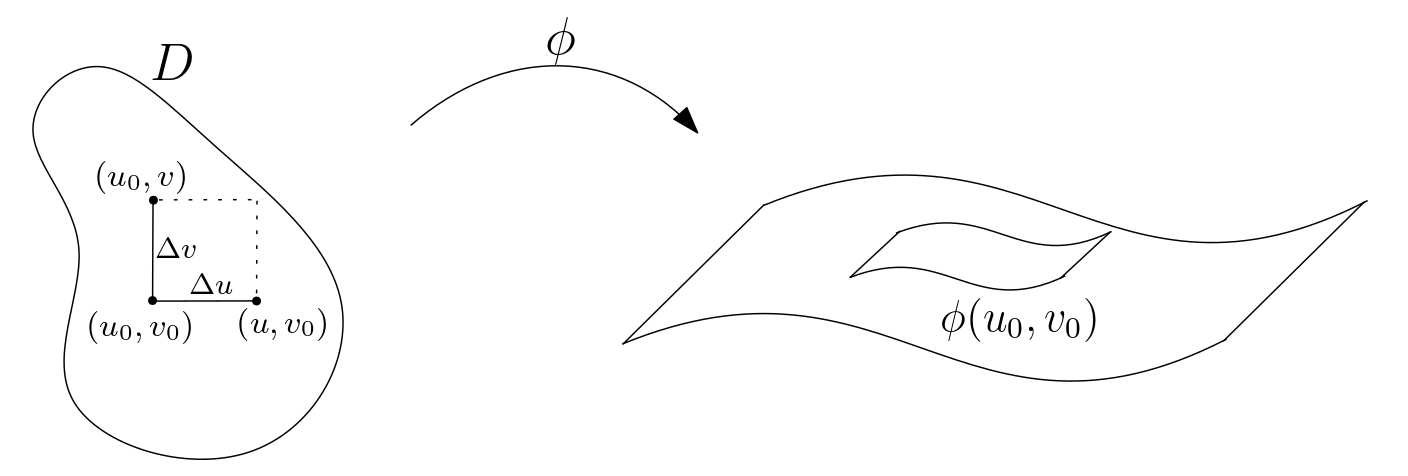
\includegraphics[width=0.8\linewidth]{MATH314_Notes_Fig8.png}
					\captionsetup{margin=1cm , justification = raggedright} \caption{TODO}
				\end{figure}
				\begin{align*}
					\varphi(u,v_{0}) \approxeq \varphi(u_{0},v_{0}) + \vec{T}_{u}\Delta u \implies & \varphi(u,v_{0}) - \varphi(u_{0},v_{0}) \approxeq \vec{T}_{u}\Delta u. \\
					\text{Similarly, }&\varphi(u_{0},v) -\varphi(u_{0},v_{0}) \approxeq \vec{T}_{v}\Delta v.
				\end{align*}
				We want to find are of the parallelogram formed by $\vec{T}_{v}\Delta v$ and $\vec{T}_{u}\Delta u$.
				\begin{align*}
					\text{Area} &= \norm{\vec{T}_{u}\Delta u \cross \vec{T}_{v}\Delta v} = \det 
					\begin{vmatrix}
						\vec{i} & \vec{j} & \vec{k} \\ 
						\pdv{x}{u}\Delta u & \pdv{y}{u}\Delta u & \pdv{z}{u} \Delta u \\
						\pdv{x}{v}\Delta v & \pdv{y}{v}\Delta v & \pdv{z}{v} \Delta v
					\end{vmatrix}
					&= \norm{\vec{T}_{u} \cross \vec{T}_{v}} \Delta u \Delta v.
				\end{align*}
				
				\begin{definition}[Surface Area]
					We define the surface area of a parameterized surface by 
					\begin{equation} 
					\iint\limits_{D} \norm{\vec{T}_{u} \cross \vec{T}_{v}}\ dudv,
					\end{equation}
					where $\norm{\vec{T}_{u} \cross \vec{T}_{v}}$ is the standard Euclidian norm of the vector $\vec{T}_{u} \cross \vec{T}_{v}$.
				\end{definition}
				
				\begin{example}
					Compute the surface area of a sphere of raidus $a$. 
					
					\noindent Here we'll use spherical coordinates. Let 
					$$ x = a\sin \varphi \cos \theta ,\quad y = a\sin\varphi\sin\theta,\quad z=a\cos \varphi.$$
					The bounds of integration are then defined from 
					$$ D := \{(\theta, \varphi) | 0 \le \theta \le 2\pi , \ \ 0\le \varphi \le \pi \}$$
					Following Definition 10.4, we must compute $\vec{T}_{\theta}, \vec{T}_{\varphi} , \vec{T}_{\theta} \cross \vec{T}_{\varphi}$ and $\norm{\vec{T}_{\theta} \cross \vec{T}_{\varphi}}.$
					\begin{align*}
						\vec{T}_{\varphi} &= (a\cos\varphi\cos \theta . a\cos \varphi \sin\theta, -a\sin\varphi) \\
						\vec{T}_{\theta} &= (-a\sin\varphi\sin\theta ,a\sin\varphi\cos\theta, 0) \\
						\vec{T}_{\varphi} \cross \vec{T}_{\theta} &= \det 
						\begin{vmatrix}
							\vec{i} & \vec{j} & \vec{k} \\
							a\cos\varphi\cos\theta & a\cos\varphi\sin\theta & -a\sin\varphi \\
							-a\sin\varphi\sin\theta & a\sin\theta\cos\theta & 0
						\end{vmatrix} \\
						&= (a^{2}\sin^{2}\varphi \cos\theta, a^{2}\sin^{2}\varphi\sin\theta, a^{2}\sin\varphi\cos\varphi) \\
						\norm{\vec{T}_{\varphi} \cross \vec{T}_{\theta}} &= \sqrt{a^{4}\sin^{4}\varphi \cos^{2}\theta + a^{4}\sin^{4}\varphi \sin^{2}\theta + a^{4} \sin^{2}\varphi \cos^{2}\varphi} \\
						&=\sqrt{a^{4}\sin^{4}\varphi + a^{4}\sin^{2}\varphi \cos^{2}\varphi}\\
						&=a^{4}\sin^{4}\varphi + a^{4}\sin^{2}\varphi (1-\cos^{2}\varphi) = \abs{a^{2}\sin\varphi}.
					\end{align*}
					Finally, 
					\begin{align*}
						\text{Surface area } &= \int_{0}^{\pi} \int_{0}^{2\pi} \abs{a^{2}\sin\varphi} \ d\theta d\varphi \qquad \sin\varphi \ge 0 \ \text{ on } \ [0,2\pi]\\
						&= 2\pi a^{2}\int_{0}^{\pi} \sin\varphi \ d\varphi = 4\pi a^{2}.
					\end{align*}
				\end{example}
				
				\begin{definition}[Surface area of the graph of a function $f(x,y)$]
					Letting $x= u \quad y= v, \quad z= f(u,v) \implies \vec{T}_{u} =\left(1,0,\pdv{f}{u}\right) , \vec{T}_{v} = \left(0,1,\pdv{f}{v}\right).$
					Computing the determinant $\vec{T}_{u} \cross \vec{T}_{v}$ yields $\left(-\pdv{f}{u} , -\pdv{f}{v} , 1\right)$. Thus, 
					\begin{equation} 
					\text{Surface area is } \ \ \iint\limits_{D} \sqrt{\left(\pdv{f}{u}\right)^{2} + \left(\pdv{f}{v}\right)^{2} +1} \ du dv.
					\end{equation}
				\end{definition}
				
				\begin{example}
					Find the surface are of a cone in the region enclosed by $y=x, \ y= x^{2}$. Following Definition 10.5 , we must first calculate the required terms and then the answer is immediate.
					$$ f(x,y) = \sqrt{x^{2} + y^{2}} \ \ , \pdv{f}{x} = \frac{x}{\sqrt{x^{2} + y^{2}}} , \ \ \pdv{f}{y} = \frac{y}{\sqrt{x^{2} + y^{2}}}.$$
					\begin{align*}
						\therefore \ \text{Surface area   } \ \ &=\int_{0}^{1} \int_{x}^{x^{2}} \sqrt{\frac{x^{2}}{x^{2} + y^{2}} + \frac{y^{2}}{x^{2} + y^{2}} +1 } \ dy dx\\
						&= \sqrt{2} \int_{0}^{1} \int_{x}^{x^{2}} dydx = \sqrt{2}x-x^{2} \ dx = \sqrt{2}\bigg[\frac12 - \frac13\bigg] \frac{\sqrt{2}}{6}.
					\end{align*}
					
					
				\end{example}
				\begin{definition}[Surface integrals]
										If $f(x,y,z)$ is a real-valued function defined on $S$ (a surface), we define the integral fo $f$ over $S$ to be 
										\begin{equation} 
										\int\limits_{S} f(x,y,z) \ ds = \iint\limits_{D} f(\varphi(u,v)) \norm{\vec{T}_{u} \cross \vec{T}_{v}} \ du dv, \label{eq_surface_integral}
										\end{equation}
										where $S$ is given by $\varphi(D)$.
				\end{definition}
				\begin{remark}
										In Definition 10.6, if $f=1$ we recover the surface area formula from Definition 10.4.
				\end{remark}
				
				\begin{example}
					Let $x=r\cos \theta$ , $y=r\sin \theta$ and $z=\theta$ ,\\ where  $D = \{(r,\theta) \ | \ 0 \le \theta \le 2\pi , 0 \le r \le 1\}$. Let $f(x,y,z) = \sqrt{x^{2} + y^{2} +1}$, compute $\int\limits_{S} f\ ds.$
					
					\noindent As before, we first compute the necessary terms 
					\begin{gather*}
						\vec{T}_{r} = (\cos\theta , \sin\theta , 0) \ \ \ \ \vec{T}_{\theta} = (-r\sin\theta, r\cos\theta ,1) \\
						\implies \vec{T}_{r} \cross \vec{T}_{\theta} = \det 
						\begin{vmatrix}
							\vec{i} & \vec{j} & \vec{k} \\ \cos\theta & \sin\theta & 0 \\ -r\sin\theta& r\cos\theta & 1
						\end{vmatrix} = (\sin\theta , -\cos\theta, r) \ \therefore \norm{\vec{T}_{u} \cross \vec{T}_{\theta}} = \sqrt{r^{2}+1}.
					\end{gather*}
					Let us now evaluate $f$ on our surface, 
					\begin{gather*}
						f(x(r,\theta) , y(r,\theta) , z(r,\theta)) = \sqrt{r^{2}\cos^{2} \theta + r^{2}\sin^{2} \theta +1} = \sqrt{r^{2}+1 } \\
						\therefore \int_{0}^{2\pi} \int_{0}^{1} \sqrt{r^{2} +1} \sqrt{r^{2} +1} \ drd\theta = \int_{0}^{2\pi } \int_{0}^{1} r^{2} +1 \ drd\theta =\frac43 \int_{0}^{2\pi} d\theta = \frac{8\pi}{3}.
 					\end{gather*}
				\end{example}
				
				\begin{example}
					Compute $\iint\limits_{S} z^{2} \ ds $ , where $S$ is the hemisphere defined by $z= \sqrt{a^{2} -x^{2} -y^{2}}$. 
					
					\noindent We already know that spherical coordinates parameterizes the sphere, so let us use them. Set 
					\begin{gather*}
						x = a\sin\varphi\cos\theta , \ \ y = a\sin\varphi \sin\theta , \ \ z = a\cos \varphi  \ \ 
						,D = \{(\varphi , \theta) \  |  \ 0 \le \varphi \le \frac{\pi}{2} , 0 \le \theta \le 2\pi\}.
					\end{gather*}
					As seen in Example 10.3 , $\norm{\vec{T}_{\varphi} \cross \vec{T}_{\theta}} = \abs{a^{2}\sin\varphi}$. Since yet again $\sin\varphi > 0$ in our present region, we have $\norm{\vec{T}_{\varphi} \cross \vec{T}_{\theta}} =a^{2}\sin\varphi$.
					\begin{align*}
						\int_{0}^{\sfrac{\pi}{2}} \int_{0}^{\pi} a^{2}\cos^{2} \varphi a^{2} \sin \varphi \ d\theta d\varphi &= a^{4} \int_{0}^{\sfrac{\pi}{2}} \int_{0}^{\pi} \cos^{2}\varphi \sin\varphi  \ d\theta d\varphi \\
						&= 2\pi a^{4} \int_{0}^{\sfrac{\pi}{2}} \cos^{2} \varphi \sin \varphi \ d\varphi .
						\intertext{This is a common integral seen in Calc 2. Let $u = \cos \varphi$  $\implies du = -\sin\varphi \ d\varphi$, thus }
						&= -2\pi a^{4} \int_{1}^{0} u^{2} \ du = \frac{2\pi}{3} a^{4}.
					\end{align*}
				\end{example}
				
				Before moving to surface integrals of vector fields, we first discuss orientable surfaces.
				
				\begin{definition}[Oriented surface]
				\label{def_oriented_surface}
					An oriented surface is a two-sided surface with one side specified as the outside or positive side ; we call the other side the inside or negative side. At each point $(x,y,z) \in S$ there are two unit normal vectors $\vec{n}_1 , \vec{n}_{2}$, where $\vec{n}_{1} = - \vec{n}_{2}$. Each of these normals can be associated with one side of the surface.
				\end{definition}
				
				\begin{figure}[H]
					\centering
					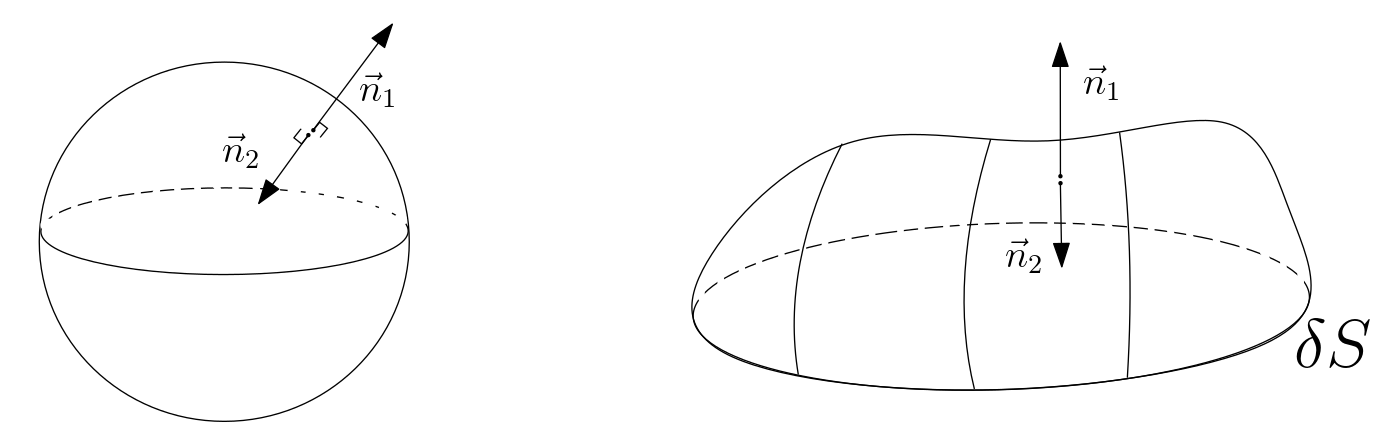
\includegraphics[width=0.8\linewidth]{MATH314_Notes_Fig9.png}
					\captionsetup{margin=1cm, justification=raggedright} \caption{\textbf{a) } Closed surface with $\vec{n}_{1}$ pointing outwards and $\vec{n}_{2}$ pointing inwards. \textbf{b) } $\vec{n}_{1}$ always points outwards and $\vec{n}_{2}$ always points inwards. To have $\vec{n}_{1}$ point inwards it would have to cross the boundary ($\delta S$).}
				\end{figure}
				
				\noindent Following Definition 10.7, a natural question is what a non-oriented surface would look like ?The Möbious strip is a classical example and is illustrated in the following figure.
				
				\begin{figure}[H]
					\centering
					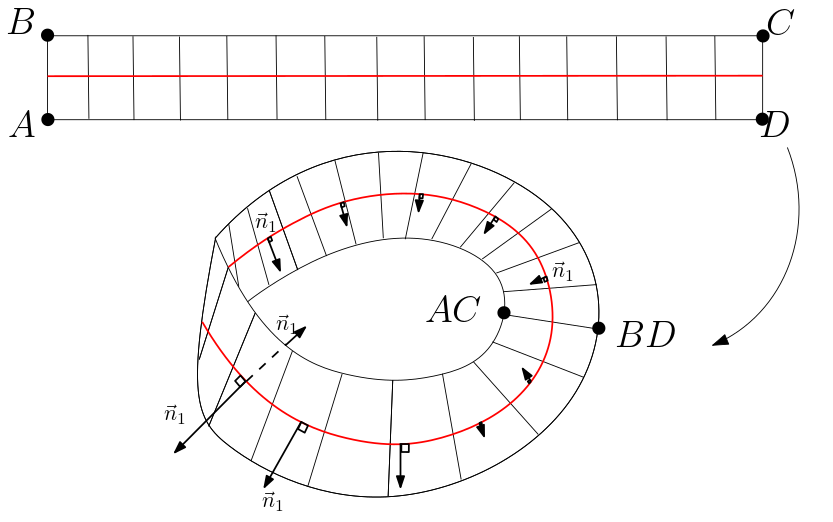
\includegraphics[width=0.8\linewidth]{MATH314_Notes_Fig10.png}
					\captionsetup{margin=1cm, justification=raggedright} \caption{\textbf{a)} A rectangular object. \textbf{b) } Twist and attach the extremities of the rectangular object to obtain the Möbius strip.}
				\end{figure}
				
				\noindent Since the Mobius strip in Figure 25 is a one-sided surface, it is not orientable.
				\\
				\noindent For a surface given by $z=g(x,y)$, we use the orientation provided by the normal vector to the tangent plane. As we did before, for 
				$$ x=u, \ y =v, \ z = g(u,v) \ \ \vec{n} = \frac{\vec{T}_{u} \cross \vec{T}_{v}}{\norm{\vec{T}_{u} \cross \vec{T}_{v}}} = \frac{\left(-\pdv{g}{u} , -\pdv{g}{v} , 1\right)}{\sqrt{\left(\pdv{g}{x}\right)^{2} + \left(\pdv{g}{y}\right)^{2} + 1}}.$$
				Since $\vec{k}$ component is positive, this gives us the upward orientation. Therefore for a parametric surface 
				\begin{equation} 
				\vec{n} = \frac{\vec{T}_{u} \cross \vec{T}_{v}}{\norm{\vec{T}_{u} \cross \vec{T}_{v}}}. \label{eq_normal_vector}
				\end{equation}
				
				\begin{example}
					Fing the outward pointing orientation for the sphere of radius one.
					\begin{gather*}
						x=a\sin\varphi\cos\theta , \ \ \ y= a\sin\varphi\sin\theta , \ \ \ z = a\cos \varphi \\
						\vec{n} = \frac{\vec{T}_{\varphi} \cross \vec{T}_{\theta}}{\norm{\vec{T}_{\varphi} \cross \vec{T}_{\theta}}} = \frac{(a^{2} \sin^{2}\varphi \cos \theta , a^{2}\sin^{2}\varphi\sin\theta , a^{2}\sin\varphi\cos\varphi)}{a^{2}\sin\varphi} \\
						\hphantom{\vec{n} = \frac{\vec{T}_{\varphi} \cross \vec{T}_{\theta}}{\norm{\vec{T}_{\varphi} \cross \vec{T}_{\theta}}}} = (\sin\varphi \cos \theta , \sin\varphi\sin\theta , \cos\varphi).
					\end{gather*}
					Indeed, as a double check
					\begin{itemize}
						\item When $\varphi = 0 \:\ (\text{Top of sphere}) \ \ \ \ \ \implies \vec{n} = (0,0,1)$
						\item When $\varphi = \pi \:\ (\text{Bottom of sphere}) \implies \vec{n} = (0,0,-1)$
						\item When $\varphi = \pi/2 \:\ (\text{Equatior}) \ \: \ \ \ \ \ \ \  \implies \vec{n} = (\cos\theta, \sin\theta , 0)$
					\end{itemize}
					$\therefore$ The surface points outward at every point using the above formula, as expected.
				\end{example}
				
				\subsection{Surface Integrals of Vector Fields}
				
				\begin{definition}[Surface integral over a vector field]
					If $\vec{F}$ is a continuous vector field defined on a oriented surface $S$ with unit normal $\vec{n}$, then the surface integral of $\vec{F}$ over $S$ is 
					\begin{equation} 
					\iint\limits_{S}F \cdot ds = \iint\limits_{S} \vec{F} \cdot \vec{n} \ ds.
					\end{equation}
					This is commonly called the \textit{flux integral across $S$}.
				\end{definition}
				
				\noindent By substituting Equation 10.1.1 in the previous definition we have 
				\begin{align}
					&\iint\limits_{S} \vec{F} \cdot ds = \iint\limits_{S} \vec{F}\cdot \abs{\frac{\vec{T}_{u} \cross \vec{T}_{v}}{\norm{\vec{T}_{u} \cross \vec{T}_{v}}}} \ ds= \iint\limits_{D} F\cdot \abs{\frac{\vec{T}_{u} \cross \vec{T}_{v}}{\norm{\vec{T}_{u} \cross \vec{T}_{v}}}} \norm{\vec{T}_{u} \cross \vec{T}_{v}} \ dA \nonumber \\
					\implies & \iint\limits_{S} \vec{F}\cdot ds = \iint\limits_{D} F \cdot (\vec{T}_{u} \cross \vec{T}_{v}) \ du dv \label{dot}. \label{eq_flux_compute}
				\end{align}
				
				\begin{remark}
					If we think of $\vec{F}$ as the velocity field of a fluid, then $F\cdot (\vec{T}_{u} \cross \vec{T}_{v})$ is a measure of the net quantity of fluid flowing outward across the surface per unit time.
				\end{remark}
				
				\begin{note}
					Essentially the dot product in Equation 10.2.1 is the projection of the vector field onto the unit normal
				\end{note}
				
				\begin{example}
					Calculate the total flux of $F= (x,y,z) $ outward through the cylinder $ x^{2}+y^{2} \le a^{2}$ with $-h \le z \le h$.
					The cylinder has three sides (top, bottom and side) so there are three different outward vectors. The top and bottom vectors are respectively $\vec{n}_{\text{top}} = (0,0,1)$ and $\vec{n}_{\text{bot}} = (0,0,-1)$. To find the side vector we let 
					$$ x = a\cos\theta , \quad y = a\sin\theta ,\quad z=z, $$
					where $\theta \in [0,2\pi]$ and $z\in [-h,h]$. Then we compute the outward vector using \eqref{eq_normal_vector}.
					\begin{align*}
						\vec{T}_{\theta}&= \la -a\sin\theta, a\cos\theta, 0 \ra \\
						\vec{T}_{z} &= \la 0,0,1 \ra \implies \vec{T}_{\theta} \cross \vec{T}_{z} = \det 
						\begin{vmatrix}
							i & j& k \\ -a\cos\theta & a\cos\theta & 0 \\ 0 & 0 & 1
						\end{vmatrix} = (a\cos\theta, a\sin\theta,0).
					\end{align*}
					Therefore, $\vec{n}_{\text{side}} = (\cos\theta, \sin\theta,0)$ as we expected.\\
					
					\noindent Now we compute each individual side flux using $\eqref{eq_flux_compute}$. \\
					(\textbf{Top}) Letting $(a\cos\theta, a\sin\theta, h)$, we have 
					\begin{align*}
						\vec{T}_{a} &= (\cos\theta, \sin\theta, 0) \quad \vec{T}_{\theta} = (-a\sin\theta, a\cos\theta , 0) \implies \vec{T}_{a} \cross \vec{T}_{\theta } = (0,0,a).\\
						\therefore &\iint\limits_{\text{Top}} F\cdot (\vec{T}_{a} \cross \vec{T}_{\theta })\ dA = \int_{0}^{2\pi} \int_{0}^{a} (x(a,\theta) , y(a,\theta) , z(a,\theta))\cdot (0,0,a) \ dad\theta \\
						&\hphantom{\iint\limits_{\text{Top}} F\cdot (\vec{T}_{a} \cross \vec{T}_{\theta })\ dA} \ = h\int_{0}^{2\pi} \int_{0}^{a} a\ dad\theta = \frac{a^{2}}{2}h \int_{0}^{2\pi} = a^{2}h\pi.
					\end{align*}
					(\textbf{Bottom}) Here The parameterization is very similar, 
						$$(a\cos\theta, a\sin\theta, -h) \implies \vec{n} = (0,0,a),$$ 
						same vector again but this time inward.
						\begin{align*}
							\therefore \vec{n} &= 0\left(\frac{\vec{T}_{a} \cross \vec{T}_{\theta}}{\norm{\vec{T}_{a} \cross \vec{T}_{\theta}}}\right) = \int_{0}^{2\pi} \int_{0}^{a} (a\cos\theta, a\sin\theta, -h) (0,0,-a)\\
							&= \int_{0}^{2\pi}\int_{0}^{a} ah \ dad\theta = a^{2}h\pi.
						\end{align*}
					\noindent(\textbf{Side})
					\begin{align*}
						\iint\limits_{\text{Side}} \vec{F}\cdot\vec{n} \ ds &= \int_{0}^{2\pi} \int_{-h}^{h} (a\cos\theta, a\sin\theta,z) \cdot(a\cos\theta,a\sin\theta, 0) \ dzd\theta \\
						&= \int_{0}^{2\pi}\int_{-h}^{h} a^{2}\cos^{2}\theta + a^{2}\sin^{2}\theta \ dzd\theta = (\dots) = 4\pi ha^{2}.
					\end{align*}
					We conclude that the total flux of the given object is $6\pi ha^{2}$.
				\end{example}
				\subsection{Stoke's Theorem}
				Stoke's theorem relates the integral around a simple closed curve $C \in \R^{3}$ to an integral over a surface $S$ for which $C$ is the boundary.
				
				\begin{note}
					Very similar to Green's theorem because integrating over a curve was related to integrating over a domain $D$.
				\end{note}
				\noindent \textbf{Recall.} The surface integral from previous classes $\eqref{eq_surface_integral}$
				$$ \int\limits_S F\cdot ds = \int\limits F\cdot \vec{n} = \int\limits_{S} F\cdot (\vec{T}_{u}\cross \vec{T}_{v}) \ ds. $$
				If $S$ is given by the surface associated with a function $f(x,y)$ then if $F = (F_{1}, F_{2}, F_{3})$ (is a vector field) then 
				\begin{equation}
					\int\limits_{S} F\cdot ds = \int\limits_{D} \left( F_{1} \left(-\pdv{z}{x}\right) + F_{2} \left(-\pdv{z}{y}\right) + F_{3}\right) \ dxdy, 
				\end{equation}				
				where $z = f(x,y)$.
				
				\noindent \textbf{Recall.} For Green's theorem we proved the result for type $3$ domains for which 
				\begin{align*}
					D &= x\in[a,b] \ \ \text{and} \ \ \varphi_{1}(x) \le y \le \varphi_{2}(x) \\
					&\hphantom{= } y\in[c,d] \ \ \text{and} \ \ \varphi_{1}(y) \le x \le \varphi_{2}(y). 
				\end{align*}
				We proved Green's theorem for this byt then we extended the result for a much larger class of domains (i.e., we partitioned into smaller domains and took the union between them Figure 19 ; Figure 20). We prove Stoke's theorem on domains where Green's theorem applies. 
				
				\begin{note}
					In this class, wherever Green's theorem applies Stoke's will apply as well even though it can be extended further.
				\end{note}
				
				\noindent Before invoking the formal definition we must clarify some concepts such as Orientation of Boundary of $S$ ($\delta S$).
				
				\noindent Suppose that $\sigma : [a,b] \to \R^{2}$, where $\sigma(t) = (x(t) , y(t))$ is a parameterization of $\delta D$. We define the parameterization of $\delta S$ as 
				\begin{equation}
					\eta : t\to (x(t), y(t), f(x(t) , y(t)).
				\end{equation}
				
				\begin{theorem}[Stoke's Theorem]
				\label{thm_stoke's_theorem}
					Let $S$ be an oriented surface (surface with defined sides $\ref{def_oriented_surface}$) defined by a $C^{2}$ function $z=f(x,y)$, where $(x,y) \in D$ and let $D$ be a $C^{1}$ vector field on $S$. Then, if $\delta S$ denotes the oriented boundart curve of $S$ as defined above then we have 
					\begin{equation}
						\int\limits_{\color{red} S} \text{curl} F\cdot d\color{red}S \color{black}= \int\limits_{\color{red}S\color{black}}(\nabla \cross F)\cdot d\color{red}S\color{black} = \int\limits_{\partial \color{blue}S}\color{black} F\cdot d\color{blue}s\color{black}
					\end{equation}
				\end{theorem}
				
				\noindent If $\eta: [a,b] \to \R^{3}$, where $\eta = (x(t) , y(t) , f(x(t) ,y(t)))$ is an orientation preserving parameterization of the simple closed curve $\delta S$ , then 
				\begin{equation}
					\int\limits_{\partial S} F\cdot ds = \int\limits_{\eta} F_{1}dx + F_{2} dy + F_{3} dz = \int_{a}^{b} \left(F_{1} \dv{x}{t} + F_{2}\dv{y}{t} + F_{3} \dv{z}{t}\right) \ dt.
				\end{equation}
				\begin{proof}
					Recalling $\eqref{eq_curl_parantheses}$ , the curl of $F$ is defined as 
					\begin{gather*}
						\text{Curl}(\vec{F}) = \left(\pdv{F_{3}}{y} - \pdv{F_{2}}{z}\right)\vec{i} +\left(\pdv{F_{1}}{z} - \pdv{F_{3}}{x}\right)\vec{j} +\left(\pdv{F_{2}}{x} - \pdv{F_{1}}{y}\right)\vec{k} \\\implies \int\limits_{S} \text{Curl} F \cdot ds = \int\limits_{D}\text{Curl} F\cdot (\vec{T}_{u} \cross \vec{T}_{v}) \ dA,
					\end{gather*} 
					where $\vec{T}_{u} \cross \vec{T}_{v} = \left(-\pdv{z}{x} , -\pdv{z}{y} , 1\right).$ 
				\begin{gather*} \therefore \int\limits_{S} \text{Curl} F\cdot ds = \int\limits_{D} \left(\pdv{F_{3}}{y} - \pdv{F_{2}}{z}\right)\left(-\pdv{z}{x}\right) + \left(\pdv{F_{1}}{z} - \pdv{F_{3}}{x}\right)\left(-\pdv{z}{y}\right) + \left(\pdv{F_{2}}{x}-\pdv{F_{1}}{y}\right) \ dA \\ 
				\hphantom{\left(\pdv{F_{3}}{y} - \pdv{F_{2}}{z}\right)\left(-\pdv{z}{x}\right) + \left(\pdv{F_{1}}{z} - \pdv{F_{3}}{x}\right)\left(-\pdv{z}{y}\right) +\left(\pdv{F_{2}}{x}-\pdv{F_{1}}{y}\right)\left(\pdv{F_{2}}{x}-\pdv{F_{1}}{y}\right)} \color{red}(\star)\color{black}.
				\intertext{Recalling that $z$ is a function of $x$ and $y$ implies that }
				\pdv{z}{y} = \pdv{z}{x}\dv{x}{t} + \pdv{z}{y}\dv{y}{t}\\
				\implies \int\limits_{\partial S}F\cdot ds = \int_{a}^{b}\left(F_{1} + F_{3} \pdv{z}{x}\right)\dv{x}{t} + \left(F_{2} + F_{3} \pdv{z}{y}\right)\dv{y}{t} \ dt \\
				\hphantom{\implies \int\limits_{\partial S} \  }= \int_{a}^{b}\underbrace{\left(F_{1} + F_{3} \pdv{z}{x}\right)}_{\mathclap{P}} dx + \underbrace{\left(F_{2}+ F_{3}\pdv{z}{y}\right)}_{\mathclap{Q}}dy 
				\implies \int\limits_{C} Pdx + Qdy = \iint\limits_{D}\pdv{Q}{x} - \pdv{P}{y} \ dA,
				\intertext{where $C$ is the boundary of $D$.}
				\end{gather*}
				Now recall that $F= \la F_{1}(x,y,z(x,y)), F_{2}(x,y,z(x,y)), F_{3}(x,y,z(x,y))\ra$, thus 
				\begin{align*}
					\pdv{Q}{x} &= \left(\pdv{F_{2}}{x} + \pdv{F_{2}}{z}\pdv{z}{x}\right) + \left(\pdv{F_{3}}{x} + \pdv{F_{3}}{z}\pdv{z}{x}\right)\pdv{z}{y} + \left(F_{3}\frac{\partial^{2}z}{\partial x \partial y}\right) \\
					\pdv{P}{y} &= \left(\pdv{F_{1}}{y} + \pdv{F_{1}}{z}\pdv{z}{y}\right) + \left(\pdv{F_{3}}{y} + \pdv{F_{3}}{z}\pdv{z}{y}\right)\pdv{z}{x} + \left(F_{3}\frac{\partial^{2} z}{\partial x \partial y}\right)\\
					\implies & \int\limits_{D} \pdv{Q}{x} - \pdv{P}{y} \ dA = \int\limits_{D} \left(\pdv{F_{2}}{z} - \pdv{F_{3}}{y}\right)\pdv{z}{x} + \left(\pdv{F_{3}}{x} - \pdv{F_{1}}{z}\right)\pdv{z}{y} + \left(\pdv{F_{2}}{x} - \pdv{F_{1}}{y}\right) dA = \color{red}(\star)\color{black}.
				\end{align*}
				\end{proof}
				
				\begin{example}
					Use Stoke's theorem to evaluate the integral $$ \int\limits_{C} -y^{3}dx + x^{3}dy - z^{3}dz,$$ where $C$ is the intersection of $x^{2}+y^{2} =1 $(cylinder) and the plane $x+y+z=1$.
					
					\noindent Note that the surface we are integrating is the plane on the domain $x^{2} + y^{2} \le 1$. Stoke's theorem says that 
					$$ \int\limits_{\partial S} F\cdot ds = \int\limits_{D}\overbrace{\text{Curl}F}^{\mathclap{\text{Vector field}}} \cdot \underbrace{(\vec{T}_{u}\cross \vec{T}_{v})}_{\mathclap{\text{Given by the plane}}}\ dA.$$
					So first and foremost we compute the curl.
					$$ \text{Curl}F = \det \begin{vmatrix}
						\vec{i} & \vec{j} & \vec{k} \\ \pdv{}{x} & \pdv{}{y} & \pdv{}{z} \\ -y^{3} & x^{2} &z^{2}
					\end{vmatrix} = 0\vec{i} - 0\vec{j} + (3x^{2} + 3y^{2})\vec{k} \implies \text{Curl }F = (0,0,3(x^{2}+y^{2})).$$
					Now for $\vec{T}_{u}\cross \vec{T}_{v}$ we have the surface $z(x,y) = 1-x-y$
					\begin{align*}
						\therefore \int\limits_{D} \text{Curl }F \cdot (\vec{T}_{u} \cross \vec{T}_{v})\ dA &= \int\limits_{S}\text{Curl }F\cdot \left(-\pdv{z}{x} , -\pdv{z}{y},1\right) \ dA = \int\limits_{D} 3x^{2} + 3y^{2} \ dA 
						\intertext{In polar coordinates , $D = \{(r,\theta) | 0 \le r \le 1, \  0\le \theta \le 2\pi\}$ therefore} 
						&= 3\int_{0}^{2\pi}\int_{0}^{1} r^{2} r \ drd\theta= \frac{3\pi}{2}.
					\end{align*}
				\end{example}
				
				\noindent Stoke's theorem also holds on parameterized surfaces given by $\Phi : D\subset \R^{2} \to S$. The orientation along $\delta S$ is induced by the orientation of th surface given by $\vec{n}$
				\begin{figure}[H]
					\centering
					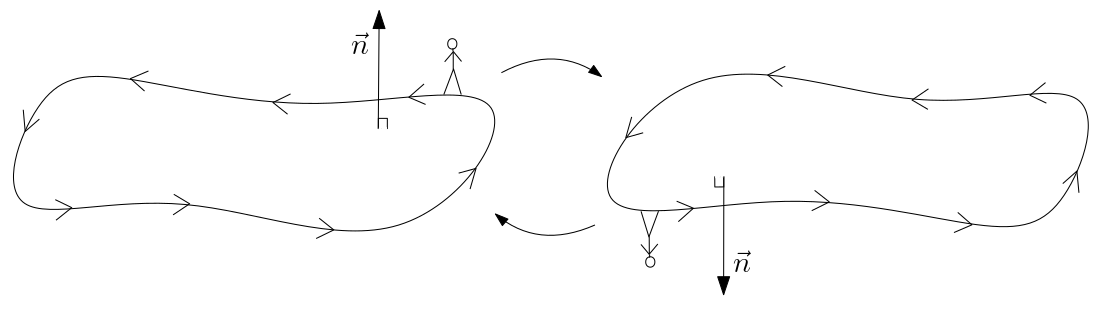
\includegraphics[width=0.9\linewidth]{MATH314_Notes_Fig11.png}
					\captionsetup{margin=1.5cm , justification=raggedright} \caption{Both sub-figures are equivalent ways of determining if a given surface has an orientation along its boundary. Standing up in the same direction as the normal vector and walking along the surface being at our left hand , implies that surface's boundary is oriented.}
				\end{figure}
				
				\begin{note}
					If we're given a parameterized surface the first thing we do is compute and outward normal.
				\end{note}
				
				\begin{example}
					Use Stoke's theorem to evaluate $\int\limits_{S} \text{Curl } F\cdot ds$, where $F=(z^{2}-1)\vec{i} + (z+xy^{3})\vec{j} + 6\vec{k}$ and $S$ is given by $x= 6-4y^{2} - 4z^{2}$ for $x\ge -2.$
				We first verify what is the orientation of the surface. Our parametrization here is $x = 6-4y^{2} -4z^{2}$ , $y=y$ and $z=z$. Therefore 
				\begin{equation*}
					\vec{T}_{y} = (-8y , 1, 0) \quad , \vec{T}_{z} = (-8z, 0,1) \quad, \vec{T}_{y} \cross \vec{T}_{z} = \det \begin{vmatrix}
						\vec{i} & \vec{j} & \vec{k} \\ 
						-8y & 1 & 0 \\ -8z & 0 & 1
					\end{vmatrix}
					= (1,8y, 8z),
				\end{equation*}
				which means the normal vector is pointing out of the surface. Now since $-2 = 6 - 4y^{2} - 4z^{2}$ , $\implies 2 = y^{2} + z^{2}$. So at $x=2$ the given surface has as boundary a circle of radius two , which can be trivially parameterized as 
				\begin{equation*}
					C(t) = (\-2, \sqrt{2} \sin(t) , \sqrt{2}\cos(t)) \qquad , 0\le t \le 2\pi.
				\end{equation*}
				Note that we knew a paraboloid has for its base a circle so it make sense to have trigonometric functions in the parameterization. This parameterization also represents the orientation of our boundary. Now by Stoke's Theorem $\eqref{thm_stoke's_theorem}$, we know that 
				$$ \int\limits_{S} \text{Curl }F \cdot ds = \int_{0}^{2\pi} F \cdot ds.$$
				\begin{align*}
					\intertext{Therefore since $\vec{F} = (z^{2}-1)\vec{i} + (z+xy^{3})\vec{j} + 6\vec{k}$ and $C'(t) = (0,\sqrt{2}\cos(t) , -\sqrt{2}\sin(t))$, we have}
					\int_{0}^{2\pi} F\cdot ds &=\int_{0}^{2\pi} F(C(t))\cdot C'(t) \ dt\\
					&=\int_{0}^{2\pi} 0 + (\sqrt(2) \cos(t) -2(\sqrt(2) \sin(t))^{3})\sqrt{2}\cos(t) - 6\sqrt{2} \sin(t) \ dt \\
					&= \int_{0}^{2\pi} 2\cos^{2}(t) - 8\sin^{3}(t) \cos(t) - 6\sqrt{2}\sin(t) \ dt \\&= \eval{\left(t + \frac{\sin(2t)}{2} - 2\sin^{4}(t) + 6\sqrt{2}\cos(t)\right)}_{0}^{2\pi} = 2\pi.
				\end{align*}
				\end{example}
			\subsection{Divergence Theorem}
				The third of the big $3$ theorems (Green's , Stokes, Divergence) is the Divergence Theorem which relates the integral of the divergence of a vector field over a solid region with a flux integral over the boundary surface(s). For example a sphere has one boundary surface while cylinders have multiple. Here we will consider solid regions $E$ which we'll name \textit{Simple solid regions}, where
				\begin{align*}
					E := &\{(x,y,z) | (x,y) \in D_{1} , u_{1} (x,y) \le z \le u_{2} (x,y)\} \\
					\text{or } &\{(x,y,z) | (x,z) \in D_{2} , v_{1} (x,z) \le y \le v_{2} (x,z)\} \\
					\text{or } &\{(x,y,z) | (y,z) \in D_{3} , w_{1} (y,z) \le x \le w_{2} (y,z)\}. \\
				\end{align*}
				Note that these can be extended to more general solids.
				
				\begin{theorem}[The Divergence Theorem]
				\label{thm_divergence}
				Let $E$ be a simple solid region and let $S$ be the boundary surface of $E$ , given with positive (outward) orientation. Let $F$ be a vector field whose component functions have continuous partials on an open set containing $E$. Then, 
				\begin{equation}
					\iint\limits_{S} F\cdot ds = \iiint\limits_{E}\text{div} F \ dV.
					\label{eq_divergence}
				\end{equation}
				Therefore the flux of $F$ across the boundary equals the integral over the solid region of the divergence of $F$.
				\end{theorem}
				\begin{note}
					Basically, if one wants to know how much air is changing inside a ball, one can either look at how much air goes in and out by the boundary (LHS of $\eqref{eq_divergence}$) or by looking at how much air is inside the ball and how is that quantity changing over time (RHS of $\eqref{eq_divergence}$).
				\end{note}
				
				\begin{proof}
					Let $F = (P,Q,R) \implies \text{div}F = \pdv{P}{x} + \pdv{Q}{y} + \pdv{R}{z}.$ Therefore, 
					\begin{gather*}
						\iiint\limits_{E} \text{div} F \ dV = \iint\limits_{E} \pdv{P}{x} \ dV +\iint\limits_{E} \pdv{Q}{y} \ dV +\iint\limits_{E} \pdv{R}{z} \ dV \\
						\text{and } \iint\limits_{S}F\cdot ds = \iint\limits_{S} F\cdot \vec{n} \ ds = \iint\limits_{S} P \vec{i} \cdot \vec{n} ds+\iint\limits_{S} Q \vec{i} \cdot \vec{n} \ ds + \iint\limits_{S} R\vec{k} \cdot \vec{n} \ ds.  
					\end{gather*}
					We prove that $$\iint\limits_{S} R\vec{k} \cdot \vec{n} \ ds = \iiint\limits_{E} \pdv{P}{z} \ dV. $$
					Since $E$ is a simple solid region this implies $E = \{(x,y,z) | (x,y) \in D , u_{1} (x,y) \le z \le u_{2}(x,y)\}.$Thus, 
					\begin{align*}
						\iiint\limits_{R} \pdv{R}{z} \ dV &= \iint\limits_{D} \bigg[\int_{u_{1}(x,y)}^{u_{2}(x,y)} \pdv{R}{z} (x,y,Z) \ dz\bigg] \ dA = \iint\limits_{D} R(x,y,u_{2}(x,y)) - R(x,y,u_{1}(x,y)) \ dA.
					\end{align*}
					\begin{figure}[H]
						\centering 
						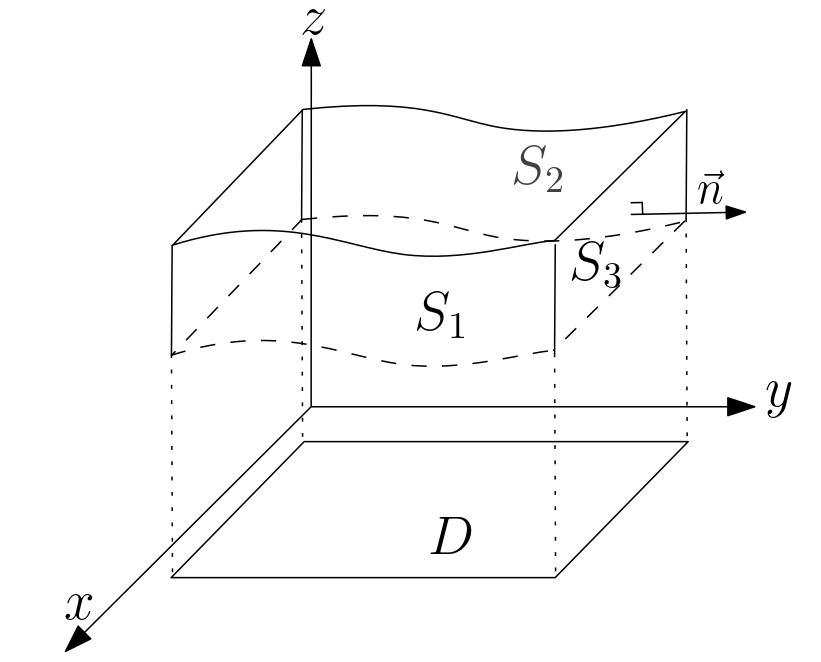
\includegraphics[width= 0.5\linewidth]{MATH314_Notes_Fig12.png}
						\captionsetup{margin=1.5cm, justification = raggedright}
						\caption{Decomposition of $\iint\limits_{S}R\vec{k}\cdot \vec{n} ds$ into three regions ; $S_{1}$ is the bottom ; $S_{2}$ is the top ; $S_{3}$ is the sides.}
					\end{figure}
					We know $S_{1}$ is given by $z = u_{1}(x,y)$ and $S_{2}$ is given by $z= u_{2}(x,y)$ (since the object is simple solid region). What about $S_{3}$?
					\begin{gather*}
						\iint\limits_{S} R \vec{k} \cdot \vec{n} \ ds = \iint\limits_{S_{1}} R \vec{k} \cdot \vec{n} \ ds + \iint\limits_{S_{2}} R \vec{k} \cdot \vec{n} \ ds + \iint\limits_{S_{3}} R \vec{k} \cdot \vec{n} \ ds
						\intertext{$S_{3}$ are are all vertical $\implies \vec{n} =$  horizontal $\implies \vec{k} \cdot \vec{n} = \vec{0}$, thus }
						 \iint\limits_{S_{3}} R\vec{k} \cdot \vec{n} \ ds = \vec{0}.
					\end{gather*}
					Therefore, 
					\begin{align*}
						\iint\limits_{S_{1}} R\vec{k} \cdot \vec{n} \ ds  &= \iint\limits_{S_{1}} \frac{-R}{\sqrt{\left(\pdv{u_{1}}{\vphantom{y}x}\right)^{2} + \left(\pdv{u_{1}}{y}\right)^{2} +1}} \ ds  \\
						&= \iint\limits_{D} \frac{-R(x,y,u_{1}(x,y))}{\sqrt{\left(\pdv{u_{1}}{\vphantom{y}x}\right)^{2} + \left(\pdv{u_{1}}{y}\right)^{2} +1}} \left(\sqrt{\left(\pdv{u_{1}}{x}\right)^{2} + \left(\pdv{u_{1}}{y}\right)^{2} +1}\right) \ dA \\
						&= \iint\limits_{S_{1}} R \vec{k} \cdot \vec{n} \ ds = \iint\limits_{D} -R (x,y,u_{1}(x,y)) \ dA.
					\end{align*}
					Similarly, 
					$$ \iint\limits_{S_{2}} R \vec{k} \cdot \vec{n} \ ds = \iint\limits_{D} R(x,y,u_{2}(x,y)) \ dA.$$
					\begin{align*}
						\therefore \iint\limits_{S} R\vec{k} \cdot \vec{n} \ ds = \iint\limits_{D} R(x,y,u_{}(x,y)) - R(x,y,u_{1}(x,y)) dA =\iiint\limits_{E} \pdv{R}{z} \ dV.
					\end{align*}
				\end{proof}
				
				\begin{example}
					Consider $\vec{F} = (2x,y^{2} ,z^{2})$. Let $S$ be the unit sphere $x^{2} +y^{2} +z^{2} =1$. Evaluate $\iint_{S} \vec{F} \cdot ds$ by using the divergence theorem. Recalling $\eqref{thm_divergence}$, 
					$$ \iint\limits_S \vec{F} \cdot ds = \iiint\limits_{E} \text{div}F \ dV.$$
					In this case, $\text{div} F = 2+ 2y +2z = 2(1+y+z)$. $E$ is the unit ball so we will use spherical coordinates
					\begin{align*}
						\iiint\limits_{E}\text{div} F \ dV &= 2 \int_{0}^{\pi}\int_{0}^{2\pi} \int_{0}^{1} (1+\rho \sin\varphi \sin\theta + \rho\cos\varphi) \rho^{2}\sin\varphi \ d\rho d\theta d\varphi \\
						&=\frac{8\pi}{3} + \int_{0}^{\pi} \int_{0}^{2\pi} \int_{0}^{1} \rho^{3}\sin^{2}\varphi \sin\theta + \rho^{3}\sin\varphi \cos\varphi \ d\rho d\theta d\varphi  
						\intertext{Trick for the above integral, the RHS has no values of $\theta$ so it is equal to $0$. The LHS has $\sin\theta\implies \eval{\cos\theta}_{0}^{2\pi} =0 \implies$ all LHS is equal to $0$.}
						\therefore \iiint\limits_{E}\text{div} F \ dV &= \frac{8\pi}{3}.
					\end{align*}
				\end{example}
				
				\begin{example}
				Evaluate $\iint\limits_{\partial w} x^{2} + y + z \ ds$, where $w$ is the unit ball $x^{2} + y^{2} + z^{2} \le 1$. Recalling $\eqref{thm_divergence}$,
				$$ \iint\limits_{\partial w} \vec{F} \cdot ds = \iiint\limits_{w} \text{div} F \ dV.$$ 
				Notice this problem is special in that we're already given $\vec{F} \cdot ds$, therefore we must find $\vec{F}$ to apply $\eqref{eq_divergence}$.Let $\vec{n}$ be the unit outward normal for the sphere $\implies \vec{n} = (x,y,z)$. Since $\vec{F} \cdot ds  = x^{2} + y +z $ , 
				$$ \implies \vec{F} \cdot \vec{n} = F_{1}x + F_{2} y + F_{3} z = x^{2} + y + z \implies \vec{F} = (x,1,1) \implies \text{div}F = 1.$$
				Finally, we apply the definition
				$$ \iint\limits_{\partial w } x^{2} + y + z \ ds = \iiint\limits_{\text{unit ball}}  1 \ dV = \frac{4\pi}{3}.$$ 
				\end{example}
				
				\begin{example}
					Evaluate $\iint\limits_{S} \vec{F} \cdot ds$ , where $F(x,y,z) = (xy^{2}, x^{2}y, y)$ and $S$ is the surface of the cylinder $x^{2} + y^{2} =1$ bounded by $z=1$ and $z=-1$.
					
					\noindent Here we must include $x^{2} + y^{2} \le 1$ on $z=1$ and $z=-1$, giving 
					\begin{align*}
						\iint\limits_{S} \vec{F} \cdot ds &= \iiint\limits_{E} \text{div} F \ dV \\
						&=\int_{-1}^{1} \bigg[\iint\limits_{\mathclap{x^{2} + y^{2} \le 1 }} \text{div}F \ dA\bigg] \ dz =\int_{-1}^{1} \bigg[\iint\limits_{\mathclap{x^{2} + y^{2} \le 1 }} x^{2} + y^{2} \ dA\bigg] \ dz
						\intertext{Let us use cylidrical coordinates to solve this, recalling \eqref{eq_cylindrical_coord} we get}
						&= \int_{-1}^{1}\int_{0}^{2\pi}\int_{0}^{1} r^{2} r \ drd\theta dz = (\dots ) = \pi.
					\end{align*}
				\end{example}
	\end{document}
